\chapter{地表湍流通量方案}\label{ch:地表湍流通量}
%\addcontentsline{toc}{chapter}{地表湍流交换过程}

%\begin{地表湍流交换过程}
\section{基本理论}\label{基本理论}
\begin{mymdframed}{代码}
  本节对应的代码文件为\texttt{MOD\_FrictionVelocity.F90}。
\end{mymdframed}

在近地层(距离地面几米到几十米高度)中,地面与大气在垂直方向存在显著的湍流输送,且湍流输送通量与风向几乎不随高度变化(固亦称常通量近地层)。
引入尺度因子,则近地层的动量通量$\left|\tau\right|$ (\unit{kg.m^{-1}.s^{-2}})、热量通量$H$ (\unit{W.m^{-2}})和水汽通量$E$ (\unit{kg.m^{-2}.s^{-1}})可分别表示为:
\begin{equation}
  |\tau|=\rho_{\mathrm{a}} \sqrt{ \left(\overline{u^{\prime} w^{\prime}}\right)^{2} + \left(\overline{v^{\prime} w^{\prime}}\right)^{2} }=\rho_{\mathrm{a}} u_{*}^{2}
\end{equation}
(分量形式:$\tau_{\mathrm{x}}=\rho_{\mathrm{a}} \overline{u^{\prime} w^{\prime}}, \quad \tau_{\mathrm{y}}=\rho_{\mathrm{a}} \overline{v^{\prime} w^{\prime}}$)
\begin{equation}
  H=C_{\mathrm{a a}} \rho_{\mathrm{a}} \overline{\theta^{\prime} w^{\prime}}=-C_{\mathrm{a}} \rho_{\mathrm{a}} \theta_{\mathrm{*}} u_{*}
\end{equation}
\begin{equation}
  E=\rho_{\mathrm{a}} \overline{q^{\prime} w^{\prime}}=-\rho_{\mathrm{a}} q_{*} u_{*}
\end{equation}
其中$u^\prime$、$v^\prime$、$w^\prime$、$\theta^\prime$、$q^\prime$分别为纬向风速度、经向风速、垂直风速、位温和比湿的湍流脉动,
$C_{\mathrm{a}}$表示干空气的比热容(\unit{J.kg^{-1}.K^{-1}}),$\rho_{\mathrm{a}}$表示大气密度(\unit{kg.m^{-3}});$u_\ast$为湍流速度尺度(即摩擦速度)(\unit{m.s^{-1}}),$\theta_\ast$为湍流位温尺度(K),
$q_\ast$为湍流湿度尺度(\unit{kg.kg^{-1}})。$\rho_{\mathrm{a}}$可由公式$\rho_{\mathrm{a}}=\frac{P_{\mathrm{a}}-0.378e_{\mathrm{a}}}{R_{\mathrm{d}}T_{\mathrm{a}}}$计算得到,
其中$P_{\mathrm{a}}$表示大气压(Pa),$\ T_{\mathrm{a}}$表示大气温度(K),$R_{\mathrm{d}}$表示干空气气体常数(\unit{J.kg^{-1}.K^{-1}}),
$e_{\mathrm{a}}=\frac{q_{\mathrm{a}}P_{\mathrm{a}}}{0.622+0.378q_{\mathrm{a}}}$表示大气水汽分压(Pa),$q_{\mathrm{a}}$表示大气比湿(\unit{kg.kg^{-1}})。
由常通量性可知$u_\ast$、$\theta_\ast$、$q_\ast$均不随高度变化。


近地层湍流通量(动量、感热和水汽等)的计算(即$u_\ast$,$\theta_\ast$,$q_\ast$的表达)主要以Monin--Obukhov相似理论为基础。
根据Monin--Obukhov相似理论,无量纲平均风速($\left|u\right|/u_\ast$)、位温($\theta/\theta_\ast$)、比湿($q/q_\ast$)的
垂直梯度可分别表达为仅依赖于参数$\zeta=\frac{z-d}{L}$的函数:
\begin{equation}\label{kz_u}
  \frac{\kappa (z-d)}{u_{*}} \frac{\partial|u|}{\partial z}=\phi_{\mathrm{m}}(\zeta)
\end{equation}
\begin{equation}\label{kz_theta}
  \frac{\kappa (z-d)}{\theta_{*}} \frac{\partial \theta}{\partial z}=\phi_{\mathrm{h}}(\zeta)
\end{equation}
\begin{equation}\label{kz_q}
  \frac{\kappa (z-d)}{q_{*}} \frac{\partial q}{\partial z}=\phi_{\mathrm{w}}(\zeta)
\end{equation}
其中 $\kappa$ 为 von K\'arman 常数,$z$为离地面高度(m),$d$为零平面位移(m),$L$为Monin-Obukhov长度(m):
\begin{equation}\label{ObukL}
  L=-\frac{u_{*}^{3}}{\kappa \left(\frac{g}{\overline{\theta_{\mathrm{a,v}}}}\right) \overline{\theta_{\mathrm{v}}^{\prime} w^{\prime}}}=\frac{u_{*}^{2} \overline{\theta_{\mathrm{a,v}}}}{\kappa g \theta_{\mathrm{v *}}}
\end{equation}
其中$\overline{\theta_{\mathrm{a,v}}}=\overline{\theta_{\mathrm{a}}}(1+0.61\overline{q_{\mathrm{a}}})$表示参考大气虚位温(K),
大气位温$\theta_{\mathrm{a}}$由其定义的一阶展开近似给出$\theta_{\mathrm{a}}=T_{\mathrm{a}}+0.0098z_{\mathrm{a}}$,$\theta_{\mathrm{v}}^{\prime}$为虚位温湍流脉动。$L$可表征近地层的大气层结稳定度:
在稳定条件下,湍流热通量$\overline{\theta_{\mathrm v}^\prime w^\prime}<0$,$L>0$;在不稳定条件下,
$\overline{\theta_{\mathrm v}^\prime w^\prime}>0$,$L<0$;在中性条件下,$\overline{\theta_{\mathrm v}^\prime w^\prime}=0$,$L\rightarrow\infty$。
$\theta_{\mathrm{v\ast}}$为虚温尺度(K),计算为:
\begin{equation}\label{thvstar}
  \theta_{\mathrm{v\ast}}=\theta_\ast+0.61(\overline{\theta_{\mathrm{a}}}q_\ast + \theta_\ast\overline{q_{\mathrm{a}}})
\end{equation}

相似性函数$\phi_{\mathrm x}$ ($\mathrm{x=m}$、$\rm h$和$\rm w$分别对应动量、感热和水汽)适用于任何下垫面条件,故亦称通用相似性函数,或简称通用函数,
它将近地层的湍流通量与$\left|u\right|$、$\theta$和$q$等的垂直梯度联系起来,构成了近地层湍流通量参数化的基础。在中性条件下,$\phi_{\mathrm m}=\phi_{\mathrm h}=\phi_{\mathrm w}=1$。



为计算得到$u_\ast$、$\theta_\ast$、$q_\ast$,通常将上述关于$\phi_{\mathrm m}\left(\zeta\right)$、$\phi_{\mathrm h}\left(\zeta\right)$、
$\phi_{\mathrm w}(\zeta)$的微分方程(公式~\eqref{kz_u}--\eqref{kz_q})在近地层的两个任意高度$z_1$和$z_2$ ($z_2>z_1$)进行积分,积分结果如下:
\begin{equation}
  |u|_{2}-|u|_{1}=\frac{u_{*}}{\kappa}\left[\ln \left(\frac{z_{2}-d}{z_{1}-d}\right)-\psi_{\mathrm{m}}\left(\frac{z_{2}-d}{L}\right)+\psi_{\mathrm{m}}\left(\frac{z_{1}-d}{L}\right)\right]
\end{equation}
%
\begin{equation}
  \theta_{2}-\theta_{1}=\frac{\theta_{*}}{\kappa}\left[\ln \left(\frac{z_{2}-d}{z_{1}-d}\right)-\psi_{\mathrm{h}}\left(\frac{z_{2}-d}{L}\right)+\psi_{\mathrm{h}}\left(\frac{z_{1}-d}{L}\right)\right]
\end{equation}
%
\begin{equation}
  q_{2}-q_{1}=\frac{q_{*}}{\kappa}\left[\ln \left(\frac{z_{2}-d}{z_{1}-d}\right)-\psi_{\mathrm{w}}\left(\frac{z_{2}-d}{L}\right)+\psi_{\mathrm{w}}\left(\frac{z_{1}-d}{L}\right)\right]
\end{equation}
其中函数$\psi_x\left(y\right)\ (x=\rm m,\ h,\ w)$定义为
\begin{equation}
  \psi_{x}(y)=\int_{\mathrm{0}}^{y} \frac{1-\phi_{x}(s)}{s} {\rm d} s
\end{equation}
$z_{0x}\ (x={\rm m,\ h,\ w})$分别表示动量、感热和水汽的粗糙长度(m)。取$z_1$为地表高度,$z_2$为大气强迫参考(观测)高度,则有如下积分边界条件:
\begin{equation}\label{VaIni}
  \begin{array}{ll}z_{1}=z_{\mathrm{0 m}}+d:|u|_{1}=0, \quad & z_{2}=z_{\mathrm{a, m}}: |u|_{2}=V_{\mathrm{a}}=\sqrt{u_{\mathrm{a}}^{2}+v_{\mathrm{a}}^{2}+U_{\mathrm{c}}^{2}} \geqslant 0.1 \\
    z_{1}=z_{\mathrm{0 h}}+d: \theta_{1}=\theta_{\mathrm{s}}, & z_{2}=z_{\mathrm{a, h}}: \theta_{2}=\theta_{\mathrm{a}} \\
  z_{1}=z_{\mathrm{0 w}}+d: q_{1}=q_{\mathrm{s}}, & z_{2}=z_{\mathrm{a, w}}: q_{2}=q_{\mathrm{a}}\end{array}
\end{equation}
则方程\eqref{kz_u}--\eqref{kz_q}由$z_1$到$z_2$的积分结果为:
\begin{equation}\label{Va}
  V_{\mathrm{a}}=\frac{u_{*}}{\kappa}\left[\ln \left(\frac{z_{\mathrm{a, m}}-d}{z_{\mathrm{0 m}}}\right)-\psi_{\mathrm{m}}\left(\frac{z_{\mathrm{a, m}}-d}{L}\right)+\psi_{\mathrm{m}}\left(\frac{z_{\mathrm{0 m}}}{L}\right)\right]
\end{equation}
%
\begin{equation}\label{theta_atm-theta_s}
  \theta_{\mathrm{a}}-\theta_{\mathrm{s}}=\frac{\theta_{\mathrm{*}}}{\kappa}\left[\ln \left(\frac{z_{\mathrm{a, h}}-d}{z_{\mathrm{0 h}}}\right)-\psi_{\mathrm{h}}\left(\frac{z_{\mathrm{a, h}}-d}{L}\right)+\psi_{\mathrm{h}}\left(\frac{z_{\mathrm{0 h}}}{L}\right)\right]
\end{equation}
%
\begin{equation}\label{q_atm-qs}
  q_{\mathrm{a}}-q_{\mathrm{s}}=\frac{q_{*}}{\kappa}\left[\ln \left(\frac{z_{\mathrm{a, w}}-d}{z_{\mathrm{0 w}}}\right)-\psi_{\mathrm{w}}\left(\frac{z_{\mathrm{a, w}}-d}{L}\right)+\psi_{\mathrm{w}}\left(\frac{z_{\mathrm{0 w}}}{L}\right)\right]
\end{equation}
这里限制$V_{\mathrm {a}}\geqslant0.1$是为了避免太小的风速使得感热与潜热过小导致数值溢出。对流速度$U_{\mathrm {c}}$表示对流边界层中的大涡对近地层湍流通量的贡献,计算方案为:
\begin{equation}
  U_{\mathrm{c}}= \begin{cases}
    0, & \text { 当 }\ \zeta_{\mathrm{a}}=\frac{z_{\mathrm{a, m}}-d}{L} \geqslant 0 \text { 时(即稳定条件下) } \\
    \beta w_{*}, & \text { 当 }\ \zeta_{\mathrm{a}}<0 \text { 时 (即不稳定条件下) }
  \end{cases}
\end{equation}
其中$w_\ast={(\frac{-gu_\ast\theta_{\mathrm{v\ast}}z_{\mathrm {i}}}{\overline{\theta_{\mathrm{a,v}}}})}^{1/3}$为垂直速度尺度 (\unit{m.s^{-1}}),$z_{\mathrm {i}}=1000$ m 代表对流边界层高度(这里设为常数),
参数$\beta=1$。

因$L$是依赖于$u_\ast$、$\theta_\ast$、$q_\ast$的函数,
故方程\eqref{Va}--\eqref{q_atm-qs}可视为如下形式的方程组:
\begin{equation}\label{FGH}
  \left\{\begin{array}{l}F\big(u_{*}, L\left(u_{*}, \theta_{*}, q_{*}\right)\big)=0 \\
      G\big(\theta_{*}, L\left(u_{*}, \theta_{*}, q_{*}\right)\big)=0 \\
  H\big(q_{*}, L\left(u_{*}, \theta_{*}, q_{*}\right)\big)=0\end{array}\right.
\end{equation}
若给$U_{\mathrm {c}}$与$L$一个初始猜测,结合大气强迫场提供的$u_{\mathrm{a}}$、$v_{\mathrm{a}}$、$\theta_{\mathrm{a}}$、$q_{\mathrm{a}}$及对应的参考高度$z_{\mathrm{a},x}\, (x=\mathrm{m,h,w})$,
地表参数$d$和$z_{0x}$的估计,以及地表$z_{0x}+d$高度$\theta_{\mathrm {s}}$、$q_{\mathrm {s}}$,则$u_\ast$、$\theta_\ast$、$q_\ast$可通过方程组
\eqref{FGH}
进行迭代求解,进而求出动量、感热和水汽通量。

根据~\citet{zeng1998intercomparison},通用函数 $\phi_x$ 有如下表达式:
\begin{equation}\label{phim_zeng}
  \phi_{\mathrm{m}}(\zeta)=\begin{cases}
    0.7 \kappa^{\frac{2}{3}}(-\zeta)^{\frac{1}{3}}, & \zeta<-1.574 \text { 时 (即非常不稳定条件下) } \\
    (1-16 \zeta)^{-\frac{1}{4}}, & -1.574 \leqslant \zeta<0 \text { 时 (即不稳定条件下) } \\
    1+5 \zeta, & 0 \leqslant \zeta \leqslant 1 \text { 时 (即稳定条件下) } \\
    5+\zeta, & \zeta>1 \text { 时 (即非常稳定条件下) }
  \end{cases}
\end{equation}
\begin{equation}
  \phi_{\mathrm{h}}(\zeta)=\phi_{\mathrm{w}}(\zeta)=\begin{cases}
    0.9 \kappa^{\frac{4}{3}}(-\zeta)^{-\frac{1}{3}}, & \zeta<-0.465 \text { 时 (即非常不稳定条件下) } \\
    (1-16 \zeta)^{-\frac{1}{2}}, & -0.465 \leqslant \zeta<0 \text { 时 (即不稳定条件下) } \\
    1+5 \zeta, & 0 \leqslant \zeta \leqslant 1 \text { 时 (即稳定条件下) } \\
    5+\zeta, & \zeta>1 \text { 时 (即非常稳定条件下) }
  \end{cases}
\end{equation}

将$\phi_{\mathrm m}$代入风速廓线方程~\eqref{Va},即可得到风速廓线在不同条件下的具体形式:

\noindent 非常不稳定条件下($\zeta_{\mathrm{a}}=\frac{z_{\mathrm{a,m}}-d}{L}<-1.574$)
\begin{equation}\label{Va_VU}
  V_{\mathrm{a}}=\frac{u_{*}}{\kappa}\left\{\ln \frac{-1.574 L}{z_{\mathrm{0 m}}}-\psi_{\mathrm{mu}}(-1.574)+
  1.14\left[\left(-\zeta_{\mathrm{a}}\right)^{\frac{1}{3}}-(1.574)^{\frac{1}{3}}\right]+\psi_{\mathrm{mu}}\left(\frac{z_{\mathrm{0 m}}}{L}\right)\right\}
\end{equation}
不稳定条件下($-1.574\leqslant\zeta_{\mathrm{a}}<0$)
\begin{equation}\label{Va_U}
  V_{\mathrm{a}}=\frac{u_{*}}{\kappa}\left\{\ln \frac{z_{\mathrm{a, m}}-d}{z_{\mathrm{0 m}}}-\psi_{\mathrm{mu}}\left(\zeta_{\mathrm{a}}\right)+\psi_{\mathrm{mu}}\left(\frac{z_{\mathrm{0 m}}}{L}\right)\right\}
\end{equation}
稳定条件下($0\leqslant\zeta_{\mathrm{a}}\leqslant1$)
\begin{equation}\label{Va_S}
  V_{\mathrm{a}}=\frac{u_{*}}{\kappa}\left\{\ln \frac{z_{\mathrm{a, m}}-d}{z_{\mathrm{0 m}}}+5 \zeta_{\mathrm{a}}-5 \frac{z_{\mathrm{0 m}}}{L}\right\}
\end{equation}
非常稳定条件下($\zeta_{\mathrm{a}}>1$)
\begin{equation}\label{Va_VS}
  V_{\mathrm{a}}=\frac{u_{*}}{\kappa}\left\{\left[\ln \frac{L}{z_{\mathrm{0 m}}}+5\right]+\left[5 \ln \zeta_{\mathrm{a}}+\zeta_{\mathrm{a}}-1\right]-5 \frac{z_{\mathrm{0 m}}}{L}\right\}
\end{equation}

\noindent 其中
\begin{equation}\label{Psim}
  \begin{array}{c}\psi_{\mathrm{mu}}\left(\zeta\right)=2\ln{(\frac{1+x}{2})}+\ln{\left(\frac{1+x^2}{2}\right)-2}\tan^{-1}{x}+\frac{\pi}{2} \\
  x={(1-16\zeta)}^{1/4}\end{array}
\end{equation}

将$\phi_{\mathrm h}$和$\phi_{\mathrm w}$代入温度廓线方程(\ref{theta_atm-theta_s})和水汽廓线方程(\ref{q_atm-qs}),即可得:

\noindent 非常不稳定条件下($\zeta_{\mathrm{a}}=\frac{z_{\mathrm{a,h}}-d}{L}$ 或$ \ \frac{z_{\mathrm{a,w}}-d}{L}\ <-0.465$)
\begin{equation}\label{theta_VU}
  \begin{aligned}
    &\theta_{\mathrm{a}}-\theta_{\mathrm{s}}= \\
    &\frac{\theta_{*}}{\kappa}\left\{\ln \frac{-0.465 L}{z_{\mathrm{0 h}}}-\psi_{\mathrm{hu}}(-0.465)+0.8\left[(0.465)^{-\frac{1}{3}}-\left(-\zeta_{\mathrm{a}}\right)^{-\frac{1}{3}}\right]
    +\psi_{\mathrm{hu}}\left(\frac{z_{\mathrm{0 h}}}{L}\right)\right\}
  \end{aligned}
\end{equation}
\begin{equation}\label{q_VU}
  \begin{aligned}
    &q_{\mathrm{a}}-q_{\mathrm{s}}= \\
    &\frac{q_{*}}{\kappa}\left\{\ln \frac{-0.465 L}{z_{\mathrm{0 w}}}-\psi_{\mathrm{wu}}(-0.465)+0.8\left[(0.465)^{-\frac{1}{3}}-
    \left(-\zeta_{\mathrm{a}}\right)^{-\frac{1}{3}}\right]+\psi_{\mathrm{wu}}\left(\frac{z_{\mathrm{0 w}}}{L}\right)\right\}
  \end{aligned}
\end{equation}
不稳定条件下($-0.465\leqslant\zeta_{\mathrm{a}}<0$)
\begin{equation}
  \theta_{\mathrm{a}}-\theta_{\mathrm{s}}=\frac{\theta_{*}}{\kappa}\left\{\ln \frac{z_{\mathrm{a, h}}-d}{z_{\mathrm{0 h}}}-\psi_{\mathrm{hu}}
  \left(\zeta_{\mathrm{a}}\right)+\psi_{\mathrm{hu}}\left(\frac{z_{\mathrm{0 h}}}{L}\right)\right\}
\end{equation}
\begin{equation}
  q_{\mathrm{a}}-q_{\mathrm{s}}=\frac{q_{*}}{\kappa}\left\{\ln \frac{z_{\mathrm{a, w}}-d}{z_{\mathrm{0 w}}}-
  \psi_{\mathrm{wu}}\left(\zeta_{\mathrm{a}}\right)+\psi_{\mathrm{wu}}\left(\frac{z_{\mathrm{0 w}}}{L}\right)\right\}
\end{equation}
稳定条件下($0\leqslant\zeta_{\mathrm{a}}\leqslant1$)
\begin{equation}
  \theta_{\mathrm{a}}-\theta_{\mathrm{s}}=\frac{\theta_{*}}{\kappa}\left\{\left[\ln \frac{z_{\mathrm{a, h}}-d}{z_{\mathrm{0 h}}}+5 \zeta_{\mathrm{a}}\right]-5 \frac{z_{\mathrm{0 h}}}{L}\right\}
\end{equation}
\begin{equation}
  q_{\mathrm{a}}-q_{\mathrm{s}}=\frac{q_{*}}{\kappa}\left\{\left[\ln \frac{z_{\mathrm{a, w}}-d}{z_{\mathrm{0 w}}}+5 \zeta_{\mathrm{a}}\right]-5 \frac{z_{\mathrm{0 w}}}{L}\right\}
\end{equation}
非常稳定条件下($\zeta_{\mathrm{a}}>1$)
\begin{equation}\label{theta_VS}
  \theta_{\mathrm{a}}-\theta_{\mathrm{s}}=\frac{\theta_{*}}{\kappa}\left\{\left[\ln \frac{L}{z_{\mathrm{0 h}}}+5\right]
  +\left[5 \ln \zeta_{\mathrm{a}}+\zeta_{\mathrm{a}}-1\right]-5 \frac{z_{\mathrm{0 h}}}{L}\right\}
\end{equation}
\begin{equation}\label{q_VS}
  q_{\mathrm{a}}-q_{\mathrm{s}}=\frac{q_{*}}{\kappa}\left\{\left[\ln \frac{L}{z_{\mathrm{0 w}}}+5\right]
  +\left[5 \ln \zeta_{\mathrm{a}}+\zeta_{\mathrm{a}}-1\right]-5 \frac{z_{\mathrm{0 w}}}{L}\right\}
\end{equation}
其中$\psi_{\mathrm{hu}}\left(\zeta\right)=\psi_{\mathrm{wu}}\left(\zeta\right)=2\ln{\left(\frac{1+x}{2}\right)}$,$x={(1-16\zeta)}^{1/2}$。

事实上,$L$的初始猜测可由总体理查德森数$R_{\mathrm{ib}}$与$\zeta$的关系得到\citep{arya2001introduction}。$R_{\mathrm{ib}}$表达为
\begin{equation}\label{Rib}
  R_{\mathrm{i b}}=\frac{\theta_{\mathrm{a,v}}-\theta_{\mathrm{s,v}}}{\overline{\theta_{\mathrm{a,v}}}} \frac{g\left(z_{\mathrm{a, m}}-d\right)}{V_{\mathrm{a}}^{2}}
\end{equation}
$R_{\mathrm{ib}}$与$\zeta$的关系为
\begin{equation}
  R_{\mathrm{ib}}=\zeta\left[\ln{\left(\frac{z_{\mathrm{a,h}}-d}{z_{\mathrm{0h}}}\right)-\psi_{\mathrm h}(\zeta)}\right] \left[\ln{\left(\frac{z_{\mathrm{a,m}}-d}{z_{\mathrm{0m}}}\right)-\psi_{\mathrm m}(\zeta)}\right]^{-2}
\end{equation}
其中$\psi_{\mathrm m}(\zeta)$与$\psi_{\mathrm h}(\zeta)$由不稳定条件下$\phi_{\mathrm h}\left(\zeta\right)=\phi_{\mathrm m}^2\left(\zeta\right)=\left(1-16\zeta\right)^{-\frac{1}{2}}$
与稳定条件下$\phi_{\mathrm h}\left(\zeta\right)=\phi_{\mathrm m}\left(\zeta\right)=1+5\zeta$确定,从而可以通过以下反算关系式得到$L$($L=\frac{z_{\mathrm{a,m}}-d}{\zeta}$)的初始猜测值
\begin{equation}\label{ZetaRib}
  \zeta=\begin{cases}
    \frac{R_{\mathrm{i b}} \ln \left(\frac{z_{\mathrm{a, m}}-d}{z_{\mathrm{0 m}}}\right)}{1-5 \min \left(R_{\mathrm{i b}}, 0.19\right)}, \qquad 10^{-6} \leqslant \zeta \leqslant 2, & \text{ 当 }\ R_{\mathrm{i b}} \geqslant 0\ \text{(即中性或稳定条件下)} \\
    R_{\mathrm{ib}} \ln \left(\frac{z_{\mathrm{a, m}}-d}{z_{\mathrm{0 m}}}\right),  \quad -100 \leqslant \zeta \leqslant-10^{-6}, & \text{ 当 }\ R_{\mathrm{i b}}<0\ \text{(即不稳定条件下)}
  \end{cases}
\end{equation}

以上给出了$u_\ast$、$\theta_\ast$、$q_\ast$的求解过程,于是地表与大气参考高度之间的动量、感热和水汽通量即可通过其定义求得。
事实上,根据$u_\ast$、$\theta_\ast$、$q_\ast$的表达形式,动量通量$\tau$、感热通量$H$和水汽通量$E$可写为如下阻抗形式:
\begin{equation}
  \tau_{\mathrm{x}}=-\frac{u_{\mathrm{a}}}{V_{\mathrm{a}}} \rho_{\mathrm{a}} u_{*}^{2}=-\rho_{\mathrm{a}} \frac{u_{\mathrm{a}}}{r_{\mathrm{a m}}}
\end{equation}
\begin{equation}
  \tau_{\mathrm{y}}=-\frac{v_{\mathrm{a}}}{V_{\mathrm{a}}} \rho_{\mathrm{a}} u_{*}^{2}=-\rho_{\mathrm{a}} \frac{v_{\mathrm{a}}}{r_{\mathrm{a m}}}
\end{equation}
\begin{equation}\label{SH}
  H=-C_{\mathrm{a}} \rho_{\mathrm{a}} \theta_{*} u_{\mathrm{*}}=-\rho_{\mathrm{a}} C_{\mathrm{a}} \frac{\left(\theta_{\mathrm{a}}-\theta_{\mathrm{s}}\right)}{r_{\mathrm{a h}}}
\end{equation}
\begin{equation}\label{LH}
  E=-\rho_{\mathrm{a}} q_{*} u_{*}=-\rho_{\mathrm{a}} \frac{\left(q_{\mathrm{a}}-q_{\mathrm{s}}\right)}{r_{\mathrm{a w}}}
\end{equation}
其中,空气动力学阻抗系数$r_{\mathrm{am}}$、$r_{\mathrm{ah}}$、$r_{\mathrm{aw}}$ (\unit{s.m^{-1}}) (结合方程~\eqref{Va}--\eqref{q_atm-qs})为
\begin{equation}\label{ram}
  r_{\mathrm{a m}}=\frac{1}{\kappa^{2} V_{\mathrm{a}}}\left[\ln \left(\frac{z_{\mathrm{a, m}}-d}{z_{\mathrm{0 m}}}\right)-\psi_{\mathrm{m}}\left(\frac{z_{\mathrm{a, m}}-d}{L}\right)+\psi_{\mathrm{m}}\left(\frac{z_{\mathrm{0 m}}}{L}\right)\right]^{2}
\end{equation}
\begin{equation}\label{rah}
  \begin{array}{c}r_{\mathrm{a h}}=\frac{1}{\kappa^{2} V_{\mathrm{a}}}\left[\ln \left(\frac{z_{\mathrm{a, m}}-d}{z_{\mathrm{0 m}}}\right)-\psi_{\mathrm{m}}\left(\frac{z_{\mathrm{a, m}}-d}{L}\right)+\psi_{\mathrm{m}}\left(\frac{z_{\mathrm{0 m}}}{L}\right)\right] \\ {\left[\ln \left(\frac{z_{\mathrm{a, h}}-d}{z_{\mathrm{0 h}}}\right)-\psi_{\mathrm{h}}\left(\frac{z_{\mathrm{a, h}}-d}{L}\right)+\psi_{\mathrm{h}}\left(\frac{z_{\mathrm{0 h}}}{L}\right)\right]}\end{array}
\end{equation}
\begin{equation}\label{raw}
  \begin{array}{c}r_{\mathrm{a w}}=\frac{1}{\kappa^{2} V_{\mathrm{a}}}\left[\ln \left(\frac{z_{\mathrm{a, m}}-d}{z_{\mathrm{0 m}}}\right)-\psi_{\mathrm{m}}\left(\frac{z_{\mathrm{a, m}}-d}{L}\right)+\psi_{\mathrm{m}}\left(\frac{z_{\mathrm{0 m}}}{L}\right)\right] \\ {\left[\ln \left(\frac{z_{\mathrm{a, w}}-d}{z_{\mathrm{0 w}}}\right)-\psi_{\mathrm{w}}\left(\frac{z_{\mathrm{a, w}}-d}{L}\right)+\psi_{\mathrm{w}}\left(\frac{z_{\mathrm{0 w}}}{L}\right)\right]}\end{array}
\end{equation}

为方便与地面观测资料进行比较,可定义2 m温度和湿度、以及10 m风速,它们实际上为$z_{0x}+d$以上2 m高度的温度、比湿,和10 m高度的风速,计算公式(即对原始微分方程从$z_{0x}+d$到$z_{0x}+d+2$ (或$z_{0x}+d+10$进行积分)如下:
  \begin{equation}\label{T2m}
    T_{\mathrm{2 m}}=\theta_{\mathrm{s}}+\frac{\theta_{*}}{\kappa}\left[\ln \left(\frac{2+z_{\mathrm{0 h}}}{z_{\mathrm{0 h}}}\right)-\psi_{\mathrm{h}}\left(\frac{2+z_{\mathrm{0 h}}}{L}\right)+\psi_{\mathrm{h}}\left(\frac{z_{\mathrm{0 h}}}{L}\right)\right]
  \end{equation}
  \begin{equation}\label{q2m}
    q_{\mathrm{2 m}}=q_{\mathrm{s}}+\frac{q_{*}}{\kappa}\left[\ln \left(\frac{2+z_{\mathrm{0 w}}}{z_{\mathrm{0 w}}}\right)-\psi_{\mathrm{w}}\left(\frac{2+z_{\mathrm{0 w}}}{L}\right)+\psi_{\mathrm{w}}\left(\frac{z_{\mathrm{0 w}}}{L}\right)\right]
  \end{equation}
  \begin{equation}\label{u10m}
    u_{\mathrm{10 m}}=\frac{u_{*}}{\kappa}\left[\ln \left(\frac{10+z_{\mathrm{0 m}}}{z_{\mathrm{0 m}}}\right)-\psi_{\mathrm{m}}\left(\frac{10+z_{\mathrm{0 m}}}{L}\right)+\psi_{\mathrm{m}}\left(\frac{z_{\mathrm{0 m}}}{L}\right)\right]
  \end{equation}


\section{考虑大涡影响的新理论}\label{考虑大涡影响的新理论}
\begin{mymdframed}{代码}
本节对应的代码文件为\texttt{MOD\_TurbulenceLEddy.F90}。
\end{mymdframed}

不稳定边界层的大涡对地表湍流交换具有重要影响,随着研究和认识的不断深入,本团队近年来在考虑大涡影响的基本理论方面有了新进展。\citet{liu2019further,liu2022surface}
通过引入边界层高度$z_{\mathrm {i}}$,发展了考虑大涡影响的地表湍流通量方案(图~\ref{fig:LZD2022方案概念图}),该方案需通过设置\texttt{DEF\_USE\_CBL\_HEIGHT} = .true.激活使用。包含大涡影响的动量通量-梯度关系通用函数形式为:
\begin{equation}
  \begin{aligned}
    \phi_{\mathrm{m}}(\zeta) &= B_{\mathrm{m}} (-\zeta)^{-1/2} \\[1ex]
    B_{\mathrm{m}} &= 0.0047(-\frac{z_{i}}{L})+0.1854
  \end{aligned}
\end{equation}
该方案(称为LZD2022方案)适用于不稳定条件($\zeta \leqslant -0.13$)。在弱不稳定条件下($\zeta > -0.13$),则仍然采用方程~\eqref{phim_zeng} (即Zeng1998方案)所列形式,确保
通用函数在由不稳定过渡到中性条件的连续性。
{
  \begin{figure}[htbp]
    \centering
    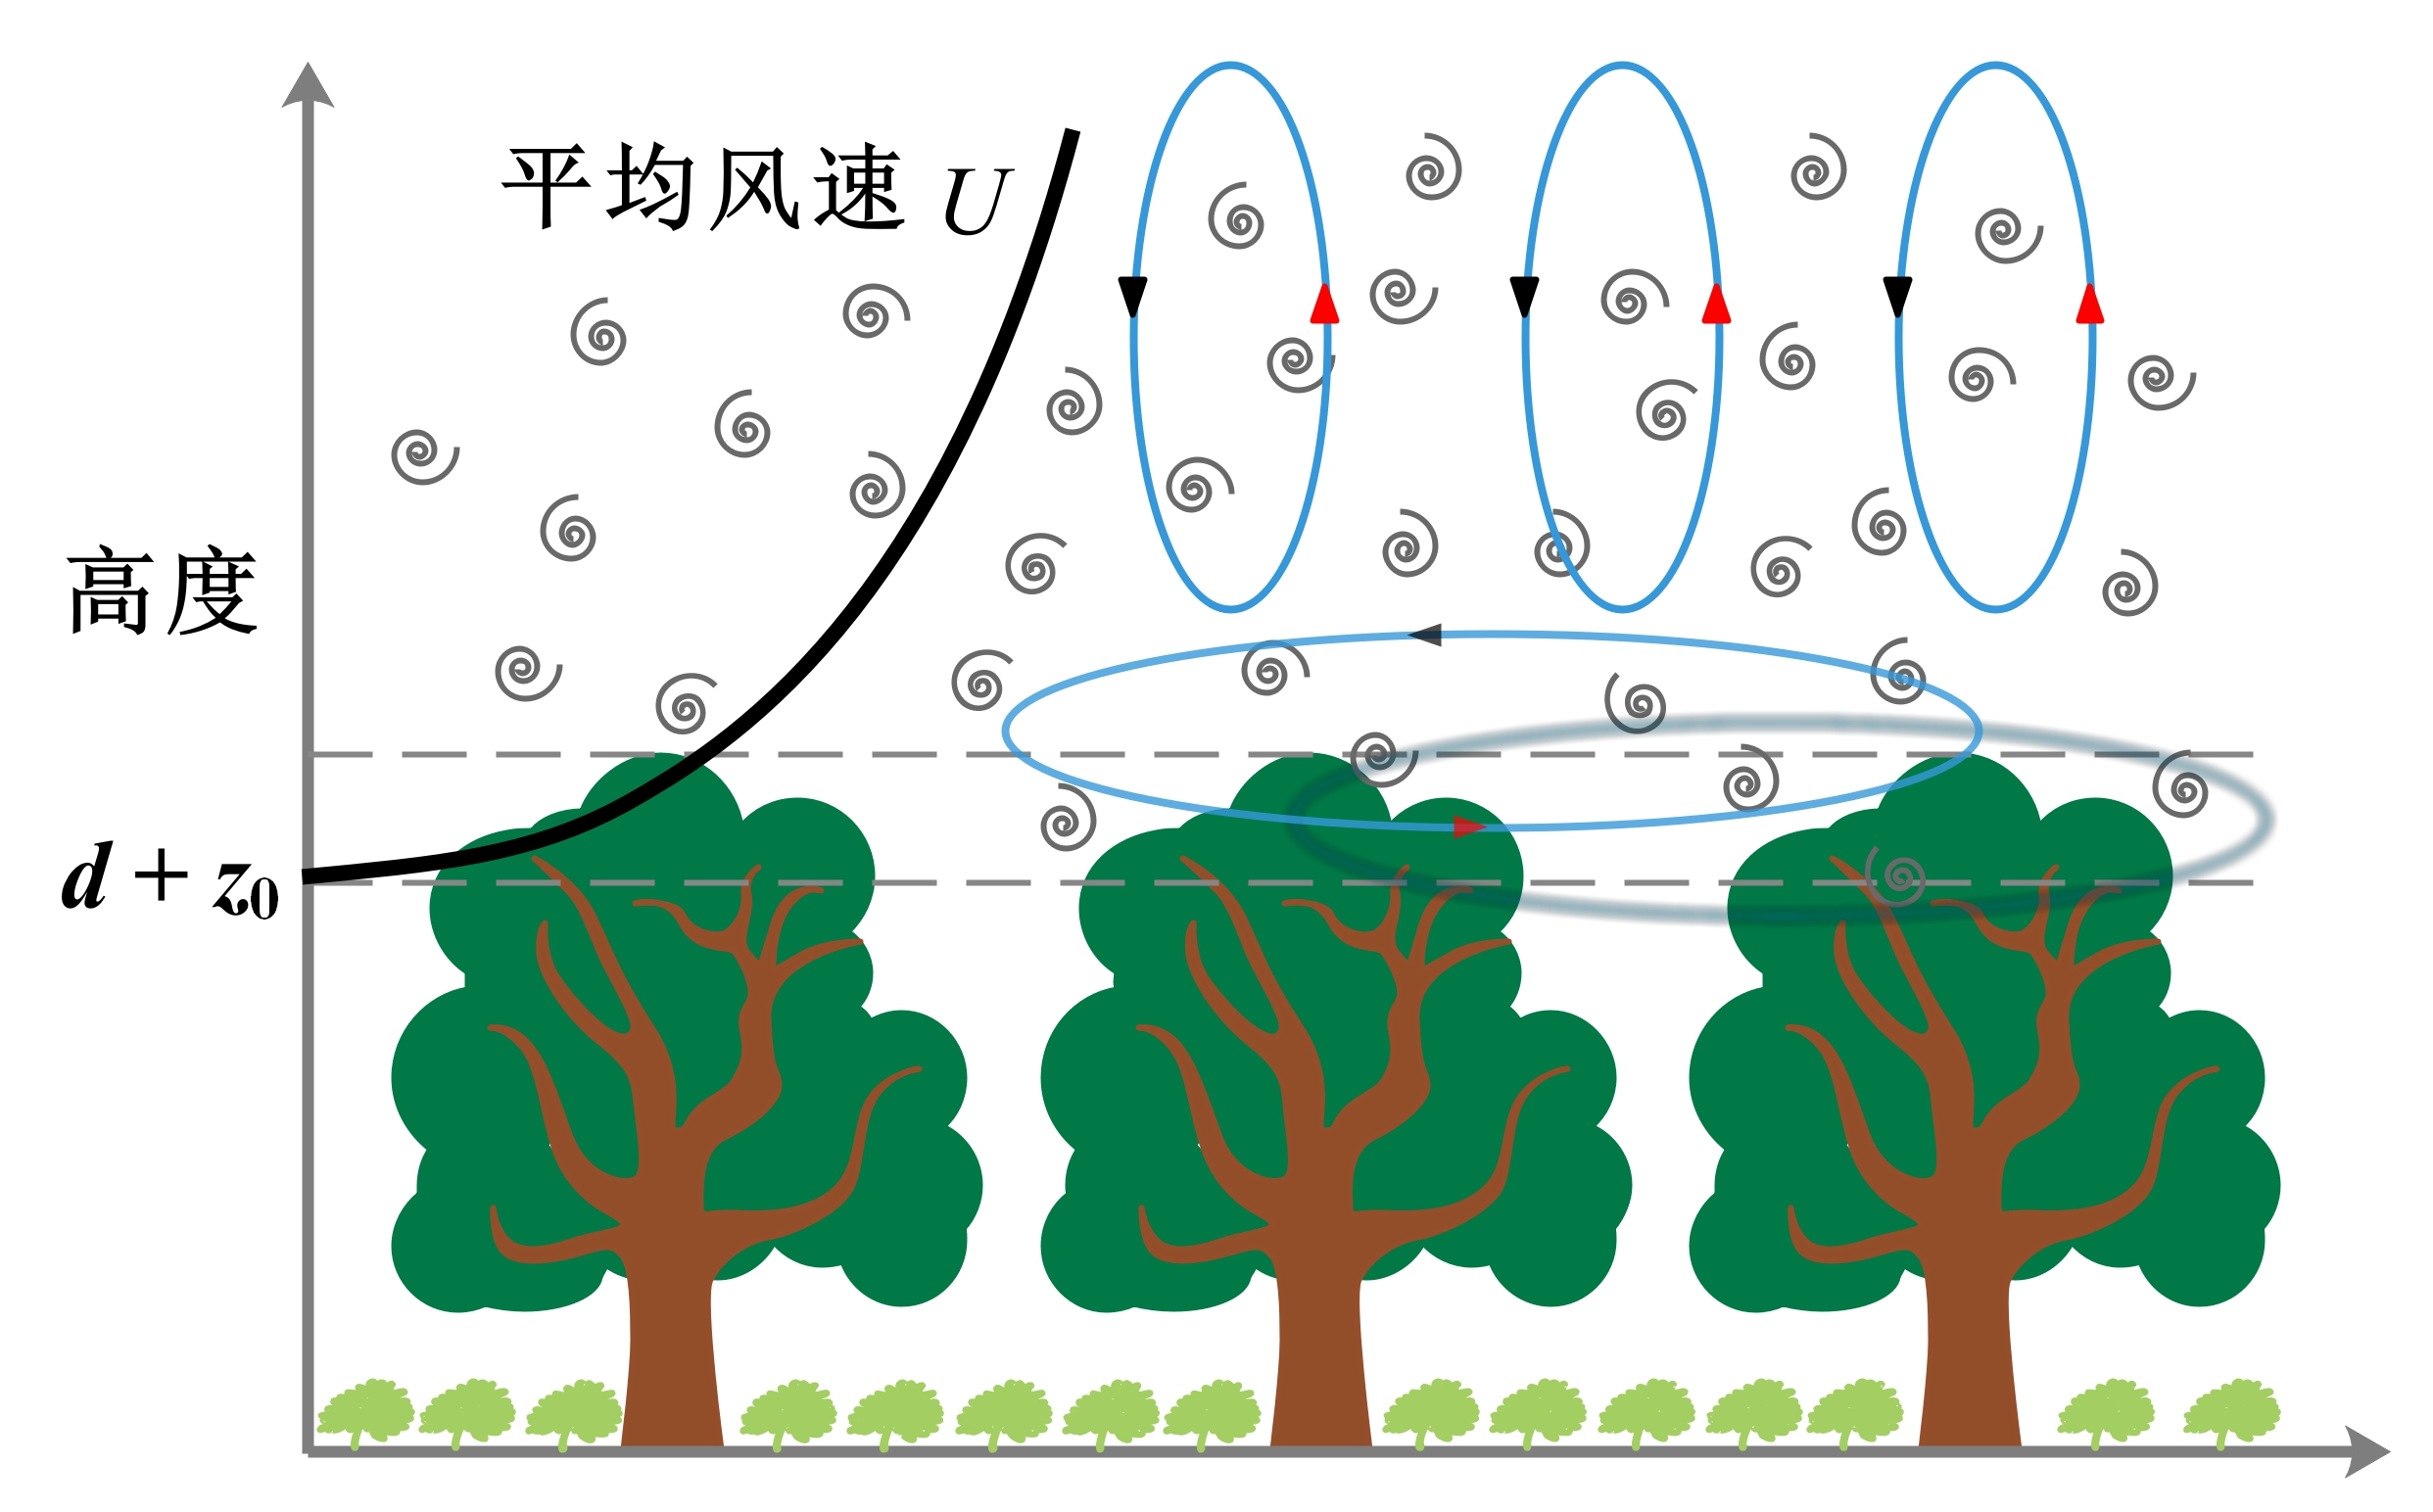
\includegraphics[scale=0.7]{Figures/地表湍流交换过程/LZD2022方案概念图.jpg}
    \caption{考虑大涡影响的地表通量方案示意图}
    \label{fig:LZD2022方案概念图}
  \end{figure}
}

根据~\citet{liu2023referenceheight},LZD2022方案曲线与Zeng1998方案的不稳定条件曲线相交(图~\ref{fig:LZD2022方案与Zeng1998方案曲线比较图}(a)),相交点的位置$\zeta_{\mathrm{m}}$与${z_{i}}/{L}$
有关(图~\ref{fig:LZD2022方案与Zeng1998方案曲线比较图}(b)),即$\zeta_{\mathrm{m}}$依赖于边界层稳定度${z_{i}}/{L}$,形式如下:
\begin{equation}
  \zeta_{\mathrm{m}}=\frac{-16-\sqrt{256+4 \left(B_{\mathrm{m}}\right)^{-4}}}{2 \left(B_{\mathrm{m}}\right)^{-4}}
\end{equation}
当相交点$\zeta_{\mathrm{m}}=-0.13$时,$B_{\mathrm{m}}=0.2722$。

结合LZD2022和Zeng1998方案,不稳定条件下($\zeta<0$)通用函数$\phi_{\mathrm{m}}$有如下表达式:
\begin{equation}
  \phi_{\mathrm{m}}(\zeta)= \begin{cases}
    B_{\mathrm{m2}}(-\zeta)^{-1/2}, & \zeta<\zeta_{\mathrm{m2}} \text { 时} \\
    (1-16 \zeta)^{-1/4}, & \zeta_{\mathrm{m2}} \leqslant \zeta<0 \text { 时} \\
  \end{cases}
\end{equation}
其中$B_{\mathrm{m2}}=\max(B_{\mathrm{m}},0.2722)$,$\zeta_{\mathrm{m2}}=\min(\zeta_{\mathrm{m}},-0.13)$,稳定条件下的$\phi_{\mathrm{m}}$则直接采用方程~\eqref{phim_zeng} 中形式。基于风速廓线方程~\eqref{Va},注意当
$\zeta_{\mathrm{a}}=\frac{z_{\mathrm{a,m}}-d}{L}<\zeta_{\mathrm{m2}}$时,方程~\eqref{Va} 中的$\psi_{\mathrm{m}}\left(\zeta_{\mathrm{a}}\right)$为:
\begin{align}
  \psi_{\mathrm{m}}\left(\zeta_{\mathrm{a}}\right) &= \int_{0}^{\zeta_{\mathrm{a}}} \frac{1-\phi_{\mathrm{m}}(s)}{s}{\mathrm d} s  \nonumber \\[1ex]
  & = \int_{0}^{\zeta_{\mathrm{m2}}} \frac{1-\phi_{\mathrm{m}}(s)}{s}{\mathrm d} s + \int_{\zeta_{\rm m2}}^{\zeta_{\mathrm{a}}} \frac{1-\phi_{\mathrm{m}}(s)}{s}{\mathrm d} s  \nonumber \\[1.5ex]
  &= \psi_{\mathrm{mu}}(\zeta_{\mathrm{m2}}) + \int_{\zeta_{\mathrm m2}}^{\zeta_{\mathrm{a}}} \frac{1-B_{\mathrm{m2}}(-s)^{-1/2}}{s}{\mathrm d} s  \nonumber \\[1.5ex]
  & = \psi_{\mathrm{mu}}(\zeta_{\mathrm{m2}}) + \ln \frac{\zeta_{\mathrm{a}}}{\zeta_{\mathrm{m2}}} + 2B_{\mathrm{m2}}\left[(-\zeta_{\mathrm{a}})^{-1/2}-(-\zeta_{\mathrm{m2}})^{-1/2}\right]
\end{align}
可得到风速廓线在不稳定条件下的具体形式:

\noindent 当$\zeta_{\mathrm{a}}<\zeta_{\mathrm{m2}}$时
\begin{equation}\label{Va_U_LZD1}
  V_{\mathrm{a}}=\frac{u_{*}}{\kappa}\left\{\ln \frac{L\zeta_{\mathrm{m2}}}{z_{\mathrm{0 m}}}-\psi_{\mathrm{mu}}\left(\zeta_{\mathrm{m2}}\right)-2B_{\mathrm{m2}}\left[(-\zeta_{\mathrm{a}})^{-1/2}-(-\zeta_{\mathrm{m2}})^{-1/2}\right]+\psi_{\mathrm{mu}}\left(\frac{z_{\mathrm{0 m}}}{L}\right)\right\}
\end{equation}
\noindent 当$ \zeta_{\mathrm{m2}} \leqslant \zeta_{\mathrm{a}}<0$时
\begin{equation}\label{Va_U_LZD2}
  V_{\mathrm{a}}=\frac{u_{*}}{\kappa}\left\{\ln \frac{z_{\mathrm{a, m}}-d}{z_{\mathrm{0 m}}}-\psi_{\mathrm{mu}}\left(\zeta_{\mathrm{a}}\right)+\psi_{\mathrm{mu}}\left(\frac{z_{\mathrm{0 m}}}{L}\right)\right\}
\end{equation}
其中$\psi_{\mathrm{mu}}$的定义同方程(\ref{Psim}),这里同样限制$V_{\mathrm {a}}\geqslant0.1$以避免风速过小问题,参考高度风速亦引入对流速度$U_{\mathrm {c}}$ (公式(\ref{VaIni})),其代表大涡在水平方向的影响,即
$V_{\mathrm{a}}=\sqrt{u_{\mathrm{a}}^{2}+v_{\mathrm{a}}^{2}+U_{\mathrm{c}}^{2}} \geqslant 0.1$。稳定条件下的风速积分形式则同方程~\eqref{Va_S} 和~\eqref{Va_VS}。

后面的迭代求解过程参见~\ref{基本理论} 节内容,所得空气动力学阻抗系数$r_{\mathrm{am}}$、$r_{\mathrm{ah}}$和$r_{\mathrm{aw}}$,以及诊断量2 m温度和湿度、10 m风速等的形式都和~\ref{基本理论} 节完全一致。
{
  \begin{figure}[htbp]
    \centering
    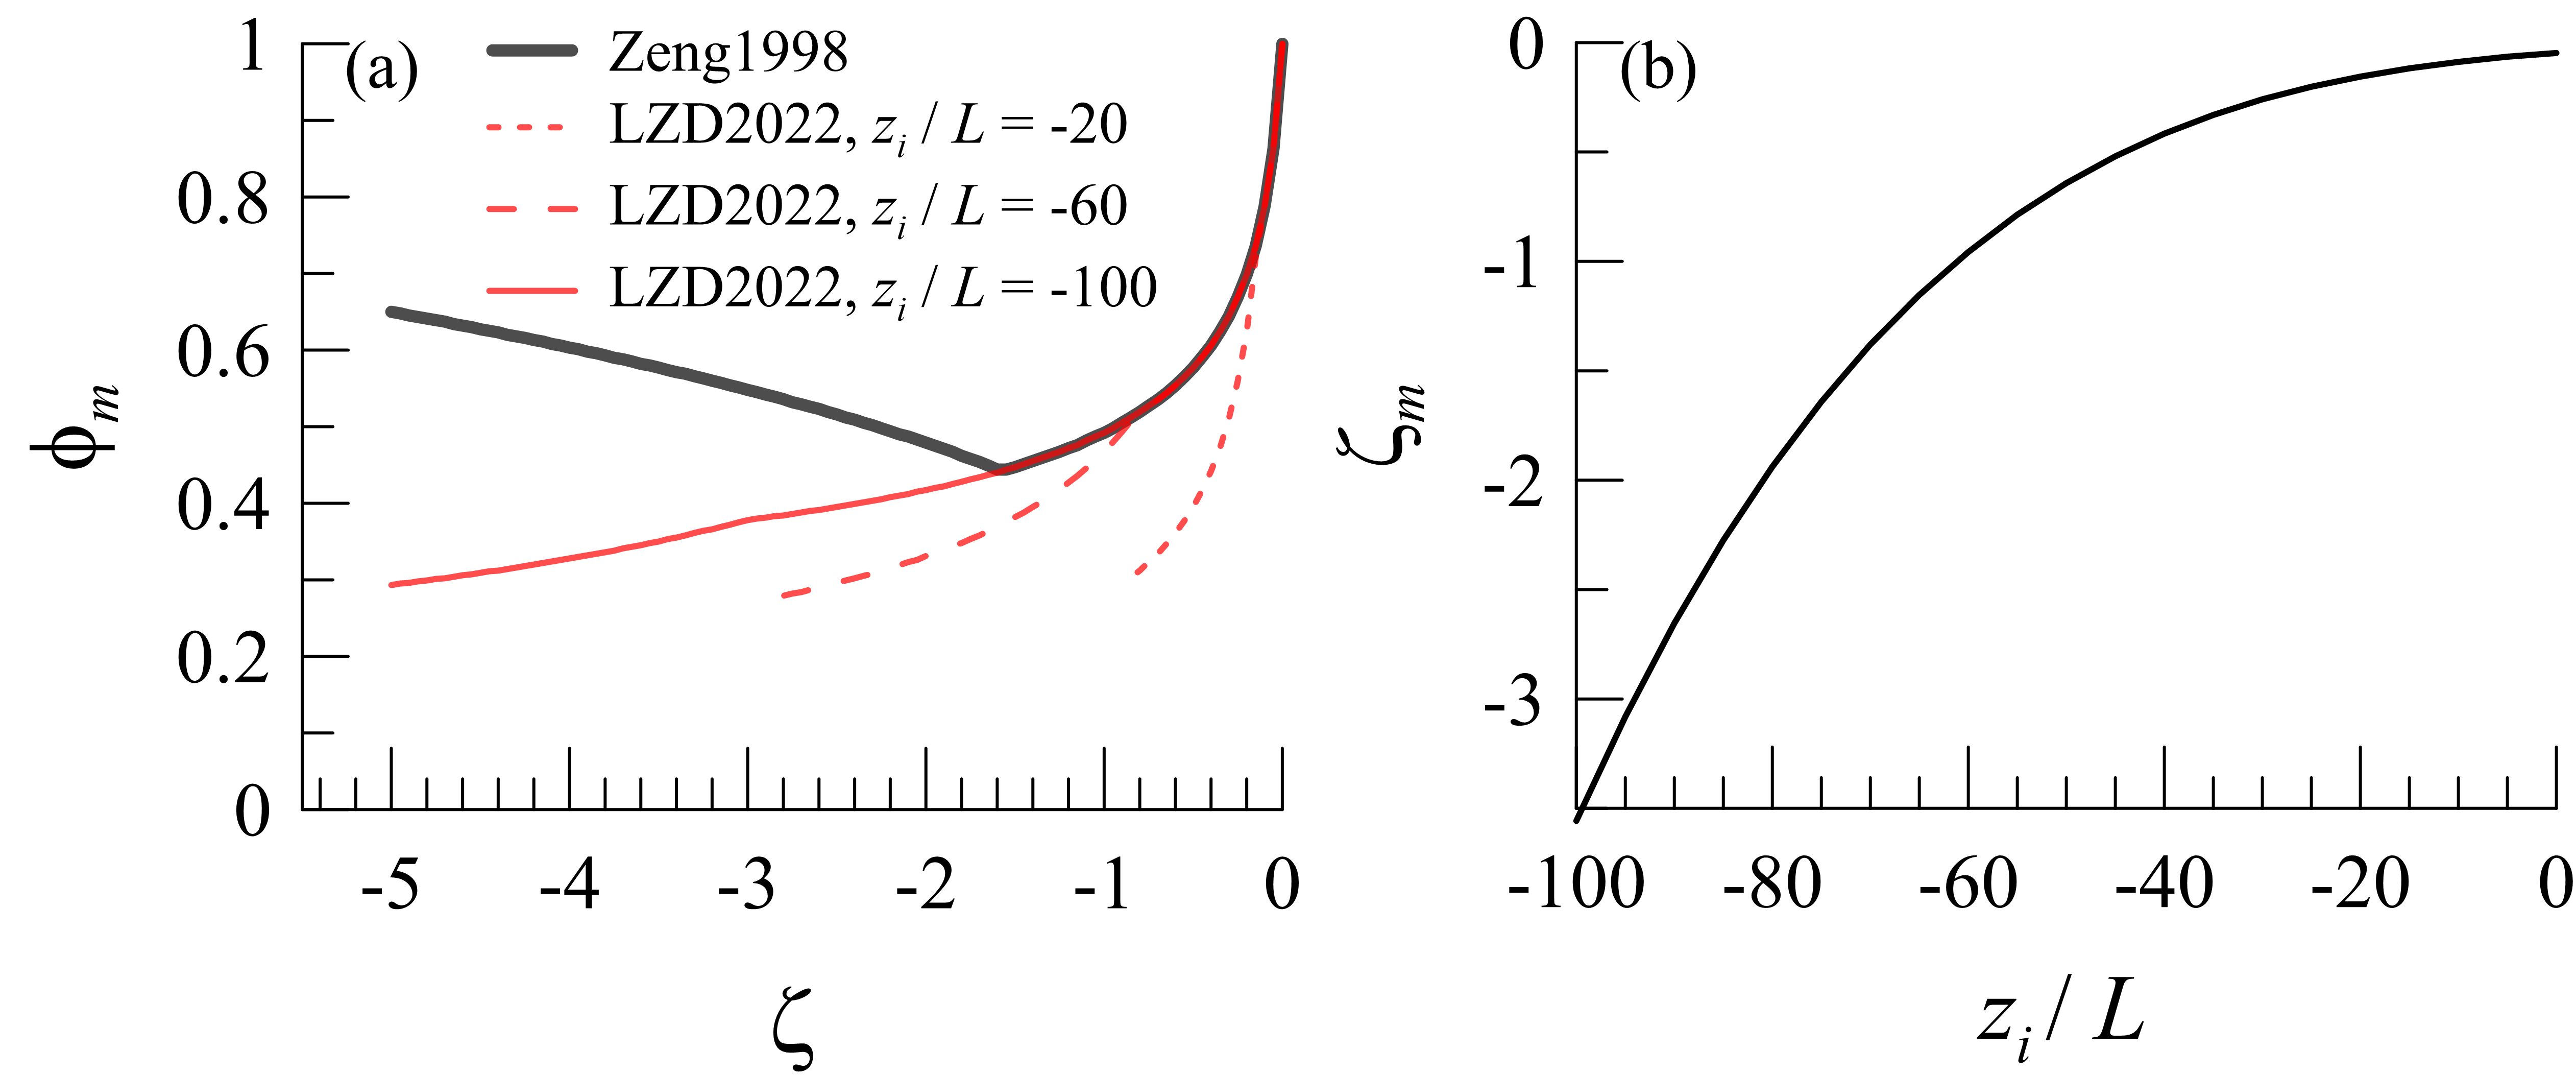
\includegraphics[scale=0.7]{Figures/地表湍流交换过程/LZD2022方案与Zeng1998方案曲线比较图.png}
    \caption{LZD2022方案与Zeng1998方案曲线比较图}
    \label{fig:LZD2022方案与Zeng1998方案曲线比较图}
  \end{figure}
}


\section{无植被覆盖地表湍流通量的计算方案}\label{无植被覆盖地表湍流通量的计算方案}
\begin{mymdframed}{代码}
  本节对应的代码文件为\texttt{MOD\_GroundFluxes.F90},部分代码包含于\texttt{MOD\_Thermal.F90}和\texttt{MOD\_SnowFraction.F90}。
\end{mymdframed}

当陆地表面没有植被覆盖(裸土、城市和湿地覆盖时)或植被已被积雪掩埋时,湍流通量按照无植被覆盖情形的方案计算。
对于任一地表类型斑块,已知植被粗糙度$z_{\mathrm{0mv}}$时,则被积雪掩埋的植被占总植被的比例为
\begin{equation}
  {\mathrm {wt}}=\frac{0.1 z_{\mathrm{{sno}}}}{z_{\mathrm{0mv}}+0.1 z_{\mathrm{{sno}}}}
\end{equation}
其中$z_{\mathrm{sno}}$表示积雪厚度(m)。CoLM2014及以前版本计算斑块中的有效植被比例$f_{\mathrm{sig}}=\left(1-{\mathrm {wt}}\right)f_{\mathrm{c}}$,无植被覆盖比例为$\left(1-f_{\mathrm{sig}}\right)$。CoLM2024版本为了考虑与PFT次网格类型的兼容性,同时认为积雪是通过覆盖或掩埋植被叶面积、茎面积进行影响,将$\rm wt$用于修正被积雪掩盖后的SAI,即${\rm SAI=TSAI}\left(1-{\mathrm {wt}}\right)$,TSAI为植被“真实”茎面积指数。当采用卫星遥感LAI时,由于其数值已经是积雪覆盖下的绿色叶面部分,故在此不对其进行积雪覆盖调整。


陆地表面可分为被积雪覆盖与未被积雪覆盖两部分。根据 \citet{swenson2012new}提供的方法,
被积雪覆盖的地表面积比例$f_{\mathrm{sno}}$可分为两步计算:在积分开始时若有降雪发生,则新一步的$f_{\mathrm{sno}}$更新为
\begin{equation}
  f_{\mathrm{{sno }}}^{(n+1)}=1-\left[1-\tanh\left(0.1 p_{\mathrm{i}} \Delta t\right)\right]\left(1-f_{\mathrm{{sno }}}^{(n)}\right) \leqslant 1.0
\end{equation}
其中$p_{\mathrm {i}}$为降雪率(\unit{kg.m^{-2}.s^{-1}}),$\Delta t$为积分步长(s);在水热过程模拟结束后,若有积雪融化发生,则$f_{\mathrm{sno}}$更新为
\begin{equation}
  f_{\mathrm{sno}}^{(n+1)}=\tanh{\left(\frac{100 z_{\mathrm{s n o}}^{2}}{2.5 z_{\mathrm{0 m, s o i}} W_{\mathrm{sno}}}\right)}
\end{equation}
其中$W_{\mathrm{sno}}$为雪水当量(mm),$z_{\mathrm{0m,soi}}$ 为未被积雪覆盖时的地表粗糙度。

对于无植被覆盖部分的陆地表面,湍流通量只存在于地表与大气之间,此部分动量通量$\tau$、感热通量$H$和水汽通量$E$表达为:
\begin{equation}\label{tau_x}
  \tau_{\mathrm{x}}=-\rho_{\mathrm{a}} \frac{u_{\mathrm{a}}}{r_{\mathrm{a m}}}
\end{equation}
\begin{equation}\label{tau_y}
  \tau_{\mathrm{y}}=-\rho_{\mathrm{a}} \frac{v_{\mathrm{a}}}{r_{\mathrm{a m}}}
\end{equation}
\begin{equation}\label{Hg}
  H_{\mathrm{g}}=-\rho_{\mathrm{a}} C_{\mathrm{a}} \frac{\theta_{\mathrm{a}}-T_{\mathrm{g}}}{r_{\mathrm{a h}}}
\end{equation}
\begin{equation}\label{Eg}
  E_{\mathrm{g}}=-\rho_{\mathrm{a}} \frac{q_{\mathrm{a}}-q_{\mathrm{g}}}{r_{\mathrm{a w}}}
\end{equation}
其中$T_{\mathrm {g}}$表示地表温度(K)。当不区分对待表层土壤和积雪时(namelist \allowbreak \texttt{DEF\_SPLIT\_\allowbreak SOILSNOW \allowbreak = \allowbreak false}),有积雪覆盖(即$f_{\mathrm{sno}}>0$)时,$T_{\mathrm {g}}$为最上层积雪的温度$T_{snl+1}$;无积雪覆盖时,$T_{\mathrm {g}}$为第一层土壤的温度$T_1$。$q_{\mathrm {g}}$表示地表空气比湿(\unit{kg.kg^{-1}}),其计算公式为:
\begin{equation}\label{qg}
  q_{\mathrm{g}}=\left(1-f_{\mathrm{{sno }}}\right) q_{\mathrm{{soil }}}+f_{\mathrm{{sno }}} q_{\mathrm{{sno }}}
\end{equation}
其中积雪表面的比湿$q_{\rm sno}$为温度在$T_{snl+1}$时的饱和比湿$q_{\mathrm{sno}}=q_{\mathrm{sat}}^{T_{snl+1}}$
(计算方案见附录~\ref{饱和水汽压(比湿)及其随温度的变化}),土壤表面的比湿$q_{\mathrm{soil}}$视为正比于温度在$T_1$时的饱和比湿:$q_{\mathrm{soil}}=\alpha_{\mathrm{soil}}q_{\mathrm{sat}}^{T_1}$,
比例系数$\alpha_{\mathrm{soil}}$为表层土壤水势$\psi_1$(mm)的函数\citep{philip1957theory}:$\alpha_{\mathrm{soil}}=\exp \left(\frac{\psi_1g}{{10}^3R_{\mathrm{v}}T_1}\right)$,
其中$R_{\mathrm{v}}$表示水汽气体常数(\unit{J.kg^{-1}.K^{-1}})。表层土壤水势$\psi_1$的计算公式为$\psi_1=\psi_{\mathrm{sat,1}}s_1^{-B_1}\geqslant-1\times{10}^8$,
$\psi_{\mathrm{sat,1}}$表示表层饱和土壤水势(mm),$B_1$表示表层土壤\citep{clapp1978empirical}参数(均由地表参数数据集提供)。$s_1$表示表层土壤对于饱和状态时的相对湿度:
\begin{equation}
  s_{1}= \begin{cases}
    0.001, & \text {如果 }\ \theta_{\mathrm{sat, 1}}<1 \times 10^{-6} \\
    \frac{1}{\Delta z_{1} \theta_{\mathrm{sat, 1}}}\left[\frac{w_{\mathrm{liq, 1}}}{\rho_{\mathrm{liq}}}+\frac{w_{\mathrm{ice, 1}}}{\rho_{\mathrm{ice}}}\right]  \text{ 且  }\  0.001 \leqslant s_{1} \leqslant 1.0, & \text {如果 }\ \theta_{\mathrm{sat, 1}} \geqslant 1 \times 10^{-6}
  \end{cases}
\end{equation}
其中$\Delta z_{1}$为表层土壤厚度(m),$\rho_{\mathrm{liq}}$和$\rho_{\mathrm{ice}}$分别为液态水和固态水密度(\unit{kg.m^{-3}}),
$w_{\mathrm{liq,1}}$和$w_{\mathrm{ice,1}}$分别为表层土壤液态水和固态水含量(\unit{kg.m^{-2}}),
$\theta_{\mathrm{sat,1}}$表示表层土壤体积含水量(即孔隙度,\unit{mm^3.mm^{-3}})。
注:为避免土壤水含量极低时轻微的土壤水变化会导致$q_{\mathrm{soil}}$变化过大,
当$q_{\mathrm{sat}}^{T_1}>q_{\mathrm{a}}$且$q_{\mathrm{a}}>q_{\mathrm{soil}}$时,取$q_{\mathrm{soil}} = q_{\mathrm{a}}$且$q_{\mathrm{soil}}$随土壤表层温度变化导数为0,即$\frac{{\rm d}q_{\mathrm{soil}}}{{\rm d}T_1} = 0$。


由于地表无植被覆盖,在计算阻抗系数$r_{\mathrm{am}}$、$r_{\mathrm{ah}}$、$r_{\mathrm{aw}}$时,零平面位移取为$d=0$。动量粗糙度在无积雪覆盖时取为$z_{\mathrm{0m}}=0.01$,有积雪覆盖(即$f_{\mathrm{sno}}>0$)时为积雪、裸土覆盖面积加权平均,即$z_{\mathrm{0m}}=0.01\left( 1-f_{\mathrm{sno}} \right )+ 0.0024 f_{\mathrm{sno}}$。
由于动量输送会受到粗糙物后面湍流波中气压波动的影响,而热量和水汽的输送过程不涉及这种动力学机制,热量和水汽必须通过界面的分子扩散进行传输,
故感热和水汽的粗糙度($z_{\mathrm{0h}}$,$z_{\mathrm{0w}}$)不同于动量粗糙度,根据~\citet{zeng1998effect}:
\begin{equation}\label{z0hw}
  z_{\mathrm{0 h}} = z_{\mathrm{0 w}} = z_{\mathrm{0 m}} \exp \left[-0.13\left(Re_{*}\right)^{0.45}\right]
\end{equation}
其中$Re_{*} = u_{*} \cdot z_{\mathrm{0 m}} / v$为粗糙雷诺数(可理解为最小湍涡的雷诺数),$\upsilon=$ \qty{1.5e-5}{(m^2.s^{-1}})为空气的动力粘性系数。


综上,无植被覆盖部分的地表湍流通量的数值计算过程可总结如下:
\begin{enumerate}
  \item 根据公式(\ref{VaIni})给出风速$V_{\mathrm{a}}$的初始猜测,其中对流速度$U_{\mathrm {c}}$的初始猜测值为:
    \begin{equation}
      U_{\mathrm{c}}= \begin{cases}
        0, & \theta_{\mathrm{a,v}}-\theta_{\mathrm{s,v}} \geqslant 0\ \text { (即稳定条件下) } \\
        0.5, & \theta_{\mathrm{a,v}}-\theta_{\mathrm{s,v}}<0\ \text { (即不稳定条件下) }
      \end{cases}
    \end{equation}
  \item 基于$R_{\mathrm{ib}}$,根据公式(\ref{Rib})和(\ref{ZetaRib}),给出Monin--Obukhov长度$L$的初始猜测;
  \item 以下过程迭代6次:\\
    a. 计算$u_\ast$ (Zeng1998方案:公式(\ref{Va_VU})-(\ref{Va_VS});LZD2022方案:公式(\ref{Va_U_LZD1})、(\ref{Va_U_LZD2})、(\ref{Va_S})--(\ref{Va_VS})) \\
    b. 计算$\theta_\ast$ (公式(\ref{theta_VU})--(\ref{theta_VS})) \\
    c. 计算$q_\ast$ (公式(\ref{q_VU})--(\ref{q_VS})) \\
    d. 更新感热和水汽粗糙度$z_{\mathrm{0h}}$、$z_{\mathrm{0w}}$ (公式~\eqref{z0hw}) \\
    e. 计算虚位温特征尺度$\theta_{\mathrm{v\ast}}$ (公式(\ref{thvstar})) \\
    f. 更新大气风速$V_{\mathrm {a}}$ (公式~\eqref{VaIni}) \\
    g. 计算新一步$L$ (公式~\eqref{ObukL}) \\
    注:每次迭代完成后,判断$L$是否改变符号,若改变符号超过4次,则视为中性条件,跳出迭代过程,以避免在稳定与不稳定条件之间来回变化;
  \item 计算空气动力学阻抗系数$r_{\mathrm{am}}$、$r_{\mathrm{ah}}$、$r_{\mathrm{aw}}$ (公式(\ref{ram})--(\ref{raw}))
  \item 计算动量通量$\tau_{\mathrm{x}}$和$\tau_{\mathrm{y}}$、感热通量$H$、水汽通量$E$ (公式(\ref{tau_x})--(\ref{Eg}))
  \item 计算地表2 m气温$T_{\mathrm{2m}}$和比湿$q_{\mathrm{2m}}$ (公式(\ref{T2m})和(\ref{q2m}))
\end{enumerate}

其后在计算地表温度并基于该温度变化对感热和水汽通量进行更新时,需提供感热和水汽通量相对地面温度的变化率,由公式(\ref{SH})和(\ref{LH})可得:
\begin{equation}
  \frac{\partial H_{\mathrm{g}}}{\partial T_{\mathrm{g}}}=\frac{\rho_{\mathrm{a}} C_{\mathrm{a}}}{r_{\mathrm{a h}}}
\end{equation}
\begin{equation}\label{Eg/Tg_1}
  \frac{\partial E_{\mathrm{g}}}{\partial T_{\mathrm{g}}}= \frac{\rho_{\mathrm{a}}}{r_{\mathrm{a w}}} \frac{{\rm d} q_{\mathrm{g}}}{{\rm d} T_{\mathrm{g}}}
\end{equation}
其中$\frac{{\rm d}q_{\mathrm {g}}}{{\rm d}T_{\mathrm {g}}}=\left[\left(1-f_{\mathrm{sno}}\right)\alpha_{\mathrm{soil}}+f_{\mathrm{sno}}\right]\frac{{\rm d}q_{\mathrm{sat}}^{T_{\mathrm {g}}}}{{\rm d}T_{\mathrm {g}}}$ (根据公式(\ref{qg})得到),$\frac{{\rm d}q_{\mathrm{sat}}^{T_{\mathrm {g}}}}{{\rm d}T_{\mathrm {g}}}$的计算见附录~\ref{饱和水汽压(比湿)及其随温度的变化}。
由于阻抗系数$r_{\mathrm{ah}}$、$r_{\mathrm{aw}}$对于温度的变化率无法解析给出,故暂时忽略。


\section{一维植被湍流交换模型}\label{一维植被湍流交换模型}
\begin{mymdframed}{代码}
  本节对应的代码文件为\texttt{MOD\_LeafTemperature.F90、MOD\_Thermal.F90}。
\end{mymdframed}

对于有植被覆盖部分的陆地表面,陆地与大气总湍流输运通量为植被冠层周围空气与大气之间的湍流输送,其动量通量$\tau$、感热通量$H$和水汽通量$E$表达为:
\begin{equation}
  \tau_{\mathrm{x}}=-\rho_{\mathrm{a}} \frac{u_{\mathrm{a}}}{r_{\mathrm{a m}}}
\end{equation}
\begin{equation}
  \tau_{\mathrm{y}}=-\rho_{\mathrm{a}} \frac{v_{\mathrm{a}}}{r_{\mathrm{a m}}}
\end{equation}
\begin{equation}
  H=-\rho_{\mathrm{a}} C_{\mathrm{a}} \frac{\theta_{\mathrm{a}}-T_{\mathrm{s}}}{r_{\mathrm{a h}}}
\end{equation}
\begin{equation}
  E=-\rho_{\mathrm{a}} \frac{q_{\mathrm{a}}-q_{\mathrm{s}}}{r_{\mathrm{a w}}}
\end{equation}
由于此时湍流通量与叶片温度耦合紧密,故阻抗系数$r_{\mathrm{am}}$、$r_{\mathrm{ah}}$、$r_{\mathrm{aw}}$与植被冠层周围($d+z_{\mathrm{0mx}}$)空气温度$T_{\mathrm {s}}$和比湿$q_{\mathrm {s}}$将随叶片温度一起采用牛顿迭代法进行求解(见章节~\ref{植被叶片温度计算})。
本节就感热与水汽通量先给出其求解的理论表达。


假设植被冠层空气的热存储能力很小并可以忽略,则它与大气之间的热量和水汽交换来源于两部分:
一是地面与植被冠层周围空气之间的湍流通量,二是植被表面(茎、叶等)与植被冠层周围空气之间的湍流通量。
对于植被的描述,植被生理过程采用 \citet{dai2004two}提出的双大叶模型,即将叶片分为阴叶(无阳光直射)与阳叶(有阳光直射)两部分。
阳叶的比例计算为:
\begin{equation}
  f_{\mathrm{sun}}=\frac{1-\exp (-K \cdot \text {LAI})}{K \cdot \text {LAI}}
\end{equation}
其中LAI为叶面积指数,$K$为直射太阳辐射消光系数(见章节~\ref{短波吸收辐射通量}),${10}^{-6}\leqslant K \cdot \text {LAI}\le40$。
当白天植被吸收的太阳辐射小于1 \unit{W.m^{-2}} 或白天结束时,$f_{\mathrm{sun}}=0.5$。叶面积指数也对应表达为两部分:
\begin{equation}
  \begin{array}{c} \text {LAI}_{\mathrm{sun}}= \text {LAI} \cdot f_{\mathrm{sun}} \\ \text {LAI}_{\mathrm{sha}}=\text {LAI} \cdot \left(1-f_{\mathrm{sun}}\right)\end{array}
\end{equation}

CoLM2014对阴阳叶分别计算温度和湍流通量。CoLM2024版本为了减少阴阳叶温度同时进行迭代的不收敛问题,并考虑与植物群落PC次网格下多种植被温度同时迭代的兼容性,植被的湍流通量与叶片温度简化为单叶模型计算,但其他过程,如辐射传输、气孔阻抗计算、植被水力等过程均为双大叶模型。湍流通量计算主要过程描述如下:

当地表有植被覆盖时,假设植被树冠水平空间分布均匀且为单层结构(即一维植被结构),则植被冠层周围空气与大气之间的感热通量$H$须等于其两项来源之和:
\begin{equation}\label{HV_balance}
  H=H_{\mathrm{g}}+H_{\mathrm{v}}
\end{equation}
其中$H_{\mathrm{g}}$表示地面与植被冠层空气顶之间的感热通量,$H_{\mathrm{v}}$表示植被冠层与其周围空气之间的感热通量,计算表达式如下:
\begin{equation}
  H_{\mathrm{g}}=-\rho_{\mathrm{a}} C_{\mathrm{a}} \frac{T_{\mathrm{s}}-T_{\mathrm{g}}}{r_{\mathrm{a h}}^{\prime}}
\end{equation}
\begin{equation}
  H_{\mathrm{v}}=-\rho_{\mathrm{a}} C_{\mathrm{a}}(\text {LAI}+\text {SAI}) \frac{T_{\mathrm{s}}-T_{\mathrm{v}}}{r_{\mathrm{b}}}
\end{equation}
其中$T_{\mathrm {v}}$表示叶片温度(K),$T_{\mathrm {s}}$表示定义在高度$z_{\mathrm{0h}}+d$上的植被冠层顶空气温度(K),SAI表示茎面积指数,$r_{\mathrm {b}}$表示叶面边界层阻抗(\unit{s.m^{-1}}),$r_{\mathrm{ah}}^\prime$(即$r_{\mathrm {d}}$)表示地表与植被冠层顶空气之间的感热阻抗(\unit{s.m^{-1}}),各部分过程如图~\ref{fig:有植被覆盖部分的陆地表面感热通量示意图} 所示。
{
  \begin{figure}[htbp]
    \centering
    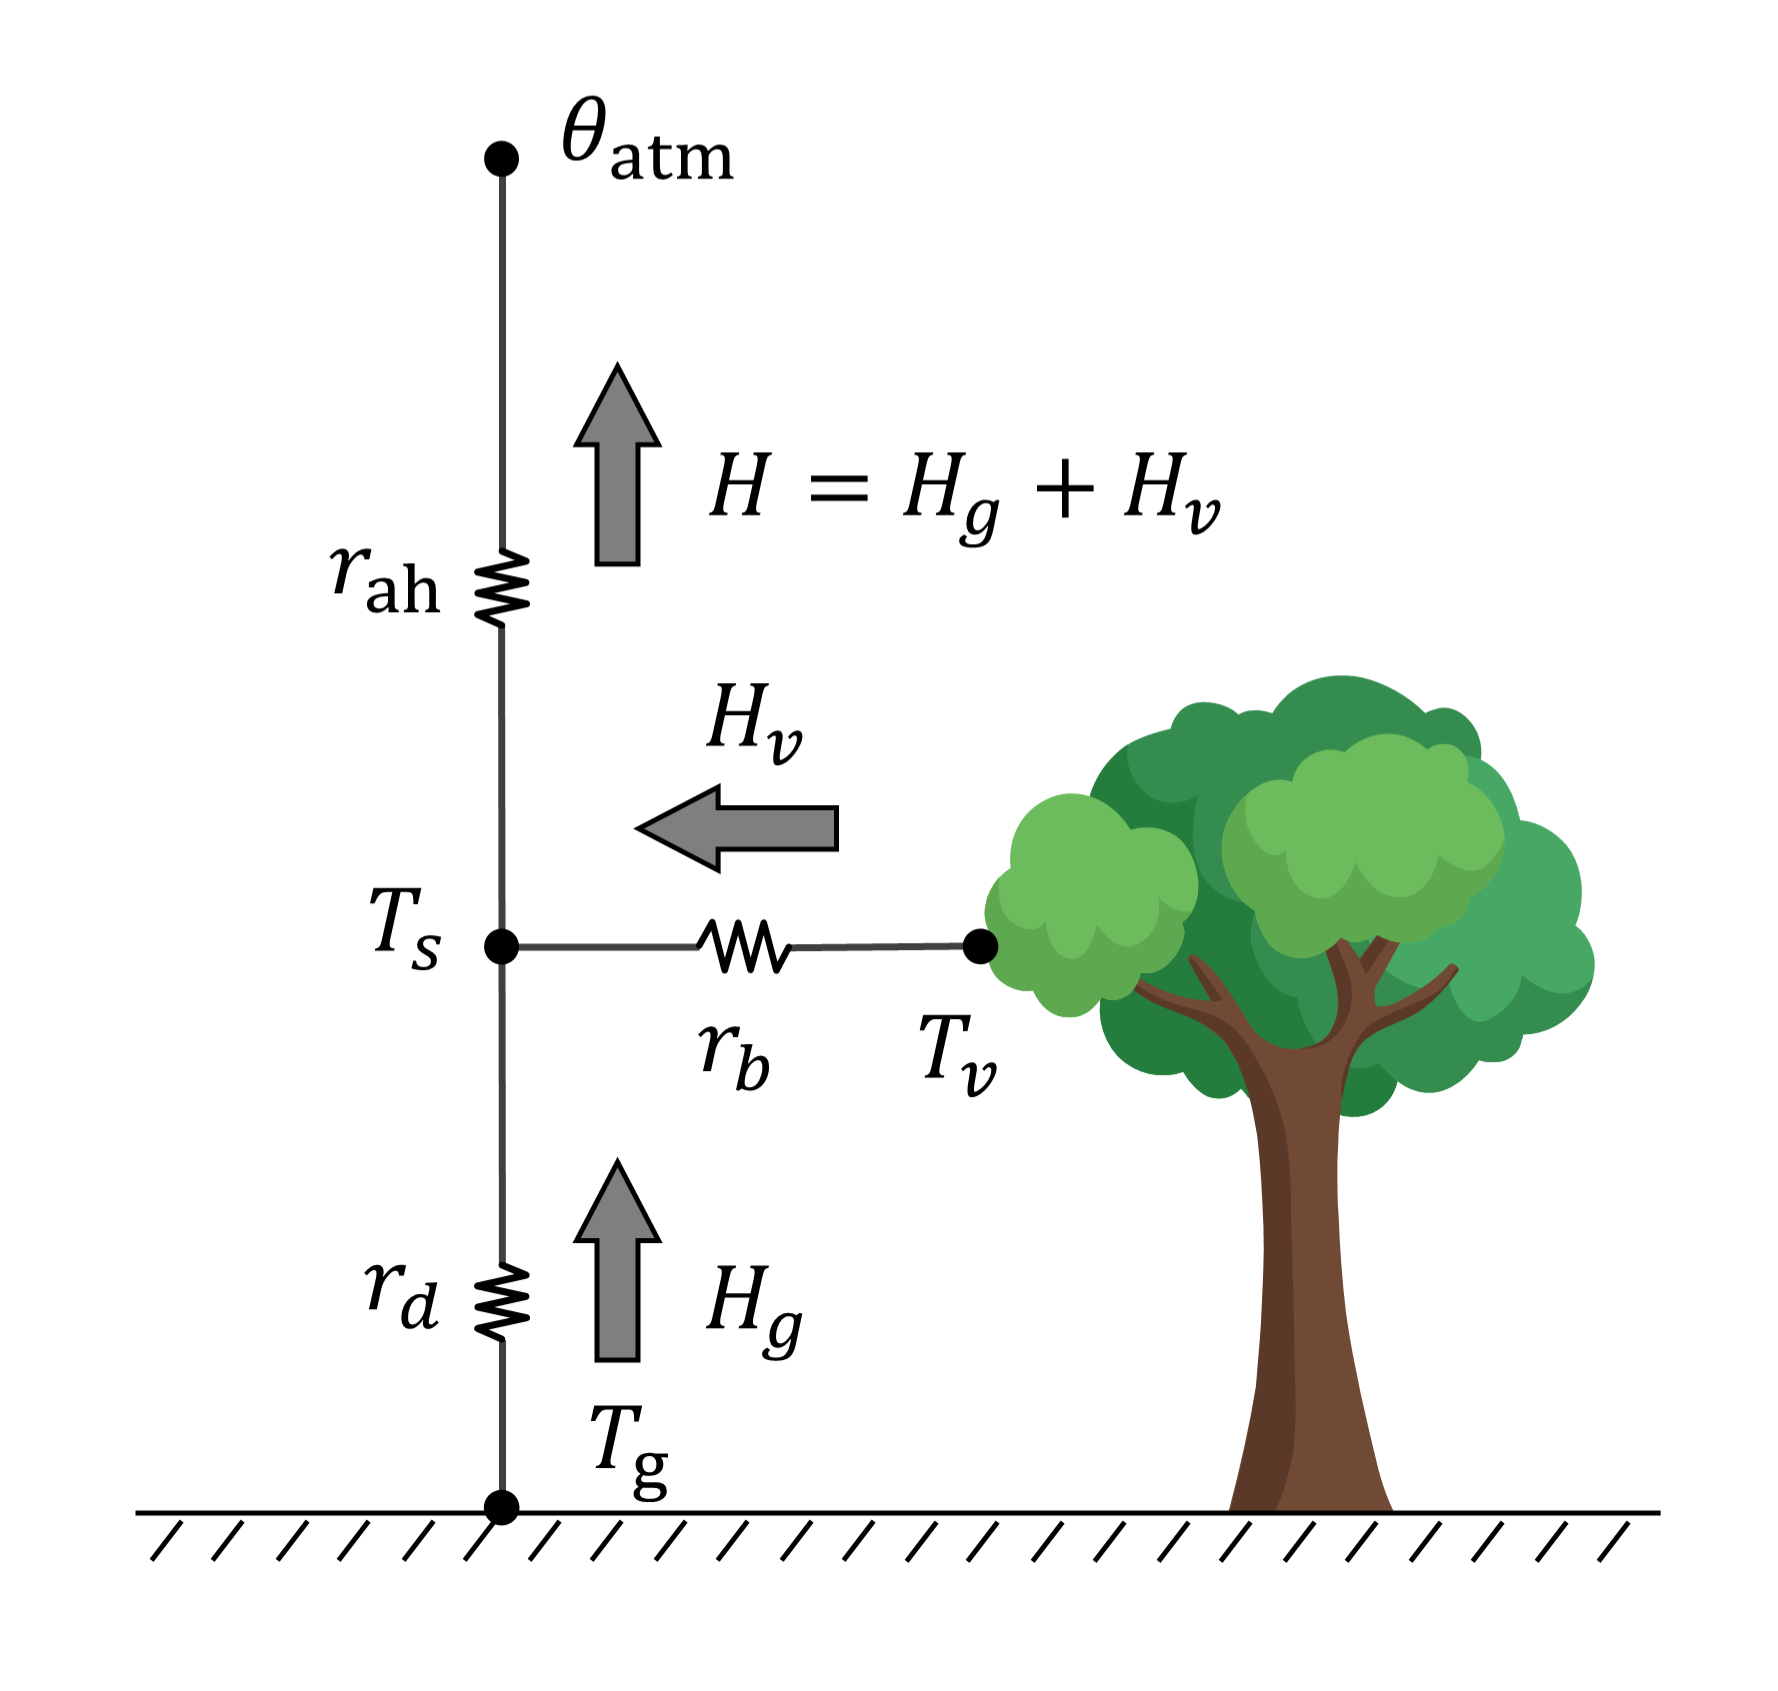
\includegraphics[width=0.6\linewidth]{Figures/地表湍流交换过程/有植被感热交换阻抗示意图.png}
    \caption{有植被覆盖时的陆地表面感热通量计算示意图}
    \label{fig:有植被覆盖部分的陆地表面感热通量示意图}
  \end{figure}
}
将$H$、$H_{\mathrm{g}}$、$H_{\mathrm{v}}$的表达式代入平衡方程(\ref{HV_balance}),即可解得$T_{\mathrm {s}}$形式如下:
\begin{equation}
  T_{\mathrm{s}}=\frac{c_{\mathrm{ah}} \theta_{\mathrm{a}}+c_{\mathrm{gh}} T_{\mathrm{g}}+c_{\mathrm{vh}} T_{\mathrm{v}}}{c_{\mathrm{ah}}+c_{\mathrm{gh}}+c_{\mathrm{vh}}}
\end{equation}
其中$c_{\mathrm{ah}}=\frac{1}{r_{\mathrm{ah}}}$,$c_{\mathrm{gh}}=\frac{1}{r_{\mathrm{ah}}^\prime}$,$c_{\mathrm{vh}}=\frac{\text {LAI}+\text {SAI}}{r_{\mathrm {b}}}$,
将$T_{\mathrm {s}}$的表达式代回,即可将$H$、$H_{\mathrm{g}}$、$H_{\mathrm{v}}$全部写为$\theta_{\mathrm{a}}$、$T_{\mathrm {g}}$、$T_{\mathrm v}$的函数,例如:
\begin{equation}
  H_{\mathrm{v}}=-\rho_{\mathrm{a}} C_{\mathrm{a}}\left[c_{\mathrm{ah}} \theta_{\mathrm{a}}+c_{\mathrm{gh}}
    T_{\mathrm{g}}+c_{\mathrm{vh}} T_{\mathrm{v}}-\left(c_{\mathrm{ah}}+c_{\mathrm{gh}}+c_{\mathrm{vh}}\right)
  T_{\mathrm{v}}\right] \frac{c_{\mathrm{vh}}}{c_{\mathrm{ah}}+c_{\mathrm{gh}}+c_{\mathrm{vh}}}
\end{equation}


同样,植被冠层周围空气与大气之间的水汽通量$E$可与另外两项平衡:
\begin{equation}\label{EV_balance}
  E=E_{\mathrm{g}}+E_{\mathrm{v}}
\end{equation}
其中$E_{\mathrm{g}}$表示地表与植被冠层周围空气之间的水汽通量,$E_{\mathrm{v}}$表示植被冠层与其周围空气之间的水汽通量:
\begin{equation}\label{eq:Eg}
  E_{\mathrm{g}}=-\rho_{\mathrm{a}} \frac{q_{\mathrm{s}}-q_{\mathrm{g}}}{r_{\mathrm{a w}}^{\prime}}
\end{equation}
\begin{equation}
  E_{\mathrm{v}}=-\rho_{\mathrm{a}} \frac{q_{\mathrm{s}}-q_{\mathrm{s a t}}^{T v}}{r_{\mathrm{vw}}}
\end{equation}
其中$q_{\mathrm{sat}}^{T_{\mathrm v}}$表示叶片温度在$T_{\mathrm v}$下的饱和比湿(\unit{kg.kg^{-1}}),$q_{\mathrm {s}}$为在高度$z_{\mathrm{0w}}+d$上的植被冠层周围空气比湿(\unit{kg.kg^{-1}}),
$q_{\mathrm {g}}$表示地面空气比湿(\unit{kg.kg^{-1}},其表达见章节~\ref{无植被覆盖地表湍流通量的计算方案}),$r_{\mathrm{aw}}^\prime$(即$r_{\mathrm {d}}$)表示地面与植被冠层顶空气之间的水汽交换阻抗 (\unit{s.m^{-1}})。
$r_{\mathrm{v}}$表示植被表面与植被冠层顶空气之间水汽交换总阻抗 (\unit{s.m^{-1}}),
它来自叶面边界层阻抗$r_{\mathrm {b}}$和气孔阻抗$r_{\mathrm{s,sun}}\left(r_{\mathrm{s,sha}}\right)$的双重贡献。
植被冠层与其周围空气之间的水汽交换包含两部分:湿的叶面及茎面的蒸发水汽交换(通过阻抗$r_{\mathrm {b}}$)和干叶表面的蒸腾水汽通量(通过阻抗$r_{\mathrm {b}}$,$r_{\mathrm{s,sun}}$和$r_{\mathrm{s,sha}}$)。
湿的叶面茎面积占总叶面茎面积的比例 \citep{dickinson1993biosphere} 为:
\begin{equation}\label{eq:fwet}
  f_{\mathrm{w e t}}=\left(\frac{W_{\mathrm{c a n}}}{W_{\mathrm{c a n, \max }}}\right)^{2 / 3} \leqslant 1.0
\end{equation}
其中$W_{\mathrm{can}}$表示植被表面储水量(\unit{kg.m^{-2}},其计算见章节~\ref{植被冠层截留}),$W_{\mathrm{can,max}}$表示植被表面最大储水量
(\unit{kg.m^{-2}}),$W_{\mathrm{can,max}}=0.1\left(\text {LAI}+ \text {SAI}\right)$。
有植被覆盖部分的陆地表面水汽通量交换过程如图~\ref{fig:有植被覆盖部分的陆地表面水汽通量示意图} 所示。
{
  \begin{figure}[htbp]
    \centering
    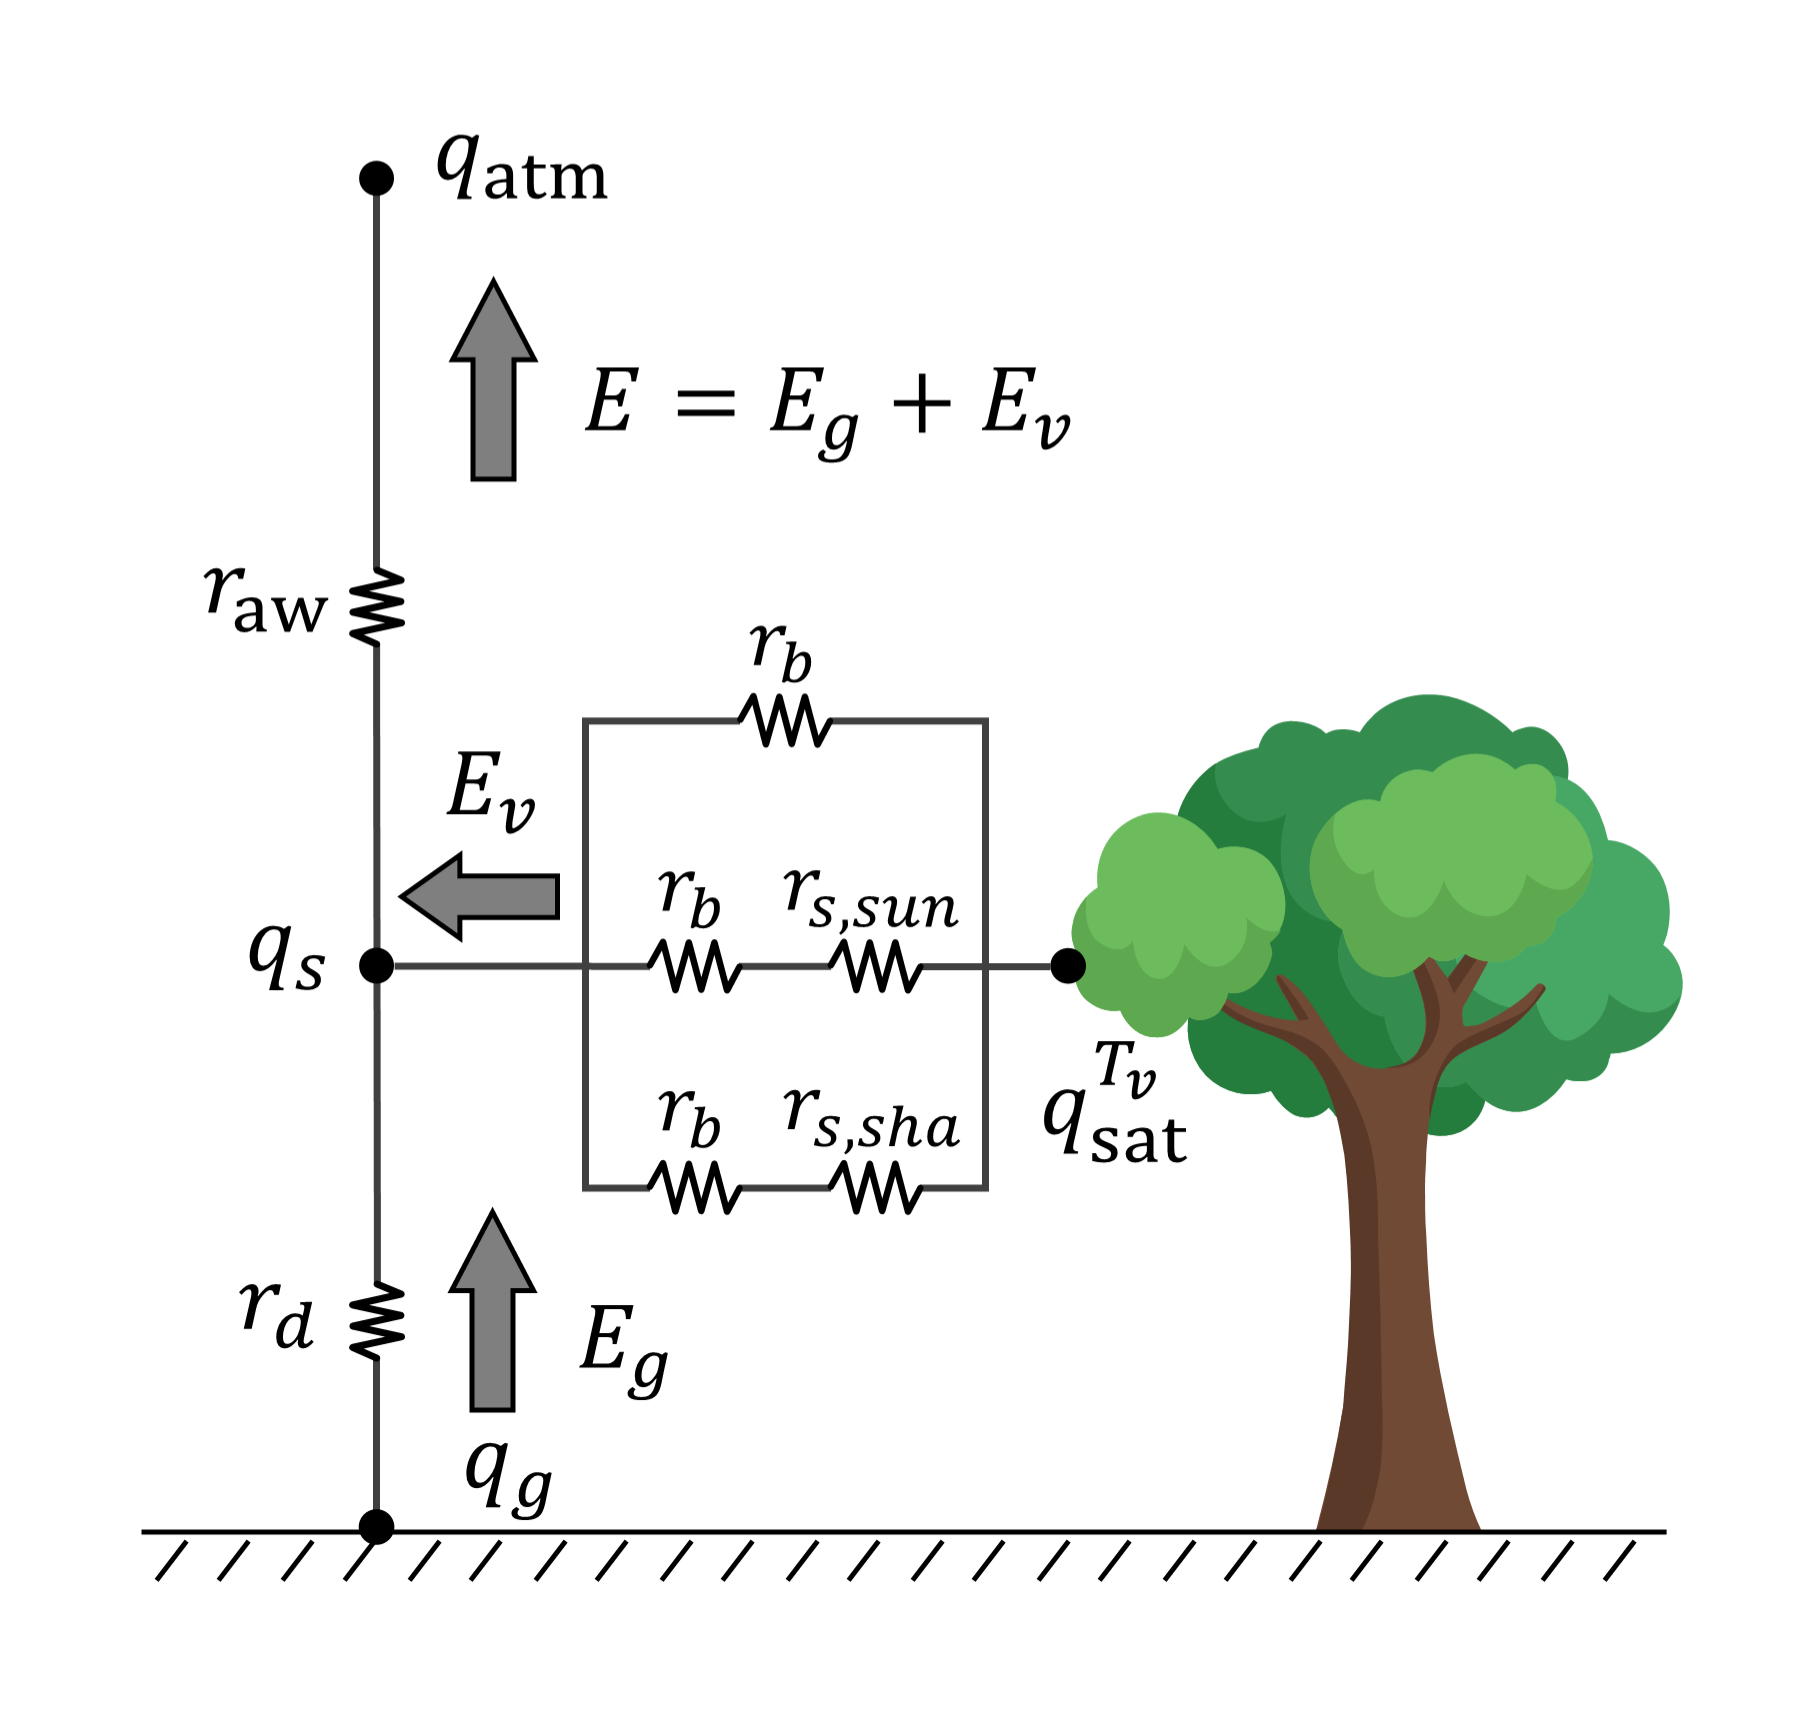
\includegraphics[width=0.6\linewidth]{Figures/地表湍流交换过程/有植被潜热交换阻抗示意图.png}
    \caption{有植被覆盖时的陆地表面水汽通量计算示意图}
    \label{fig:有植被覆盖部分的陆地表面水汽通量示意图}
  \end{figure}
}

将$E$、$E_{\mathrm{g}}$、$E_{\mathrm{v}}$的表达式代入平衡方程(\ref{EV_balance}),即可解得$q_{\mathrm {s}}$表达式如下:
\begin{equation}\label{Eg_2}
  q_{\mathrm{s}}=\frac{c_{\mathrm{aw}} q_{\mathrm{a}}+c_{\mathrm{gw}} q_{\mathrm{g}}+c_{\mathrm{vw}} q_{\mathrm{s a t}}^{T_{\mathrm{v}}}}{c_{\mathrm{aw}}+c_{\mathrm{gw}}+c_{\mathrm{vw}}}
\end{equation}
其中$c_{\mathrm{aw}}=\frac{1}{r_{\mathrm{aw}}}$,$c_{\mathrm{gw}}=\frac{1}{r_{\mathrm{aw}}^\prime}$,$c_{\mathrm{vw}}=\frac{1}{r_{\mathrm{vw}}}$,
将$q_{\mathrm {s}}$的表达式代回,即可将$E$、$E_{\mathrm{g}}$、$E_{\mathrm{v}}$全部写为$q_{\mathrm{a}}$、$q_{\mathrm {g}}$、$q_{\mathrm{sat}}^{T_{\mathrm v}}$的函数,例如:
\begin{equation}\label{Ev}
  E_{\mathrm{v}}=-\rho_{\mathrm{a}}\left[c_{\mathrm{aw}} q_{\mathrm{a}}+c_{\mathrm{gw}} q_{\mathrm{g}}+c_{\mathrm{vw}} q_{\mathrm{s a t}}^{T_{\mathrm{v}}}-
  \left(c_{\mathrm{aw}}+c_{\mathrm{gw}}+c_{\mathrm{vw}}\right) q_{\mathrm{s a t}}^{T_{\mathrm{v}}}\right] \frac{c_{\mathrm{vw}}}{c_{\mathrm{aw}}+c_{\mathrm{gw}}+c_{\mathrm{vw}}}
\end{equation}
根据植被冠层与其周围空气之间的水汽交换为湿的叶面与茎面的蒸发水汽和干叶表面的蒸腾水汽之和,$c_{\mathrm{vw}}$可由下式导出。
当$q_{\mathrm{sat}}^{T_{\mathrm v}}>q_{\mathrm {s}}$即叶片蒸散发可以发生时,%总水汽通量为叶片蒸发通量和叶片蒸腾通量之和:
\begin{equation}
  \underbrace{-\rho_{\mathrm{a}} \frac{q_{\mathrm{s}}-q_{\mathrm{s a t}}^{T_{\mathrm{v}}}}{r_{\mathrm{{v }}}}}_{\text{总水汽通量}}
  =\underbrace{-\rho_{\mathrm{a}}
  \frac{q_{\mathrm{s}}-q_{\mathrm{s a t}}^{T_{\mathrm{v}}}}{\frac{r_{\mathrm{b}}}{(\text {LAI}+\text {SAI}) \cdot f_{\mathrm{{wet }}}}}}_{\text{叶片蒸发通量}}
  \underbrace{-\rho_{\mathrm{a}} \frac{q_{\mathrm{s}}-q_{\mathrm{s a t}}^{T_{\mathrm{v}}}}{\frac{1}{\text {LAI} \cdot \left(1-f_{\mathrm{wet}}\right)\left(\frac{f_{\mathrm{sun}}}{r_{\mathrm{b}}+r_{\mathrm{s,sun}}} + \frac{f_{\mathrm{sha}}}{r_{\mathrm{b}}+r_{\mathrm{s,sha}}}\right)}}}_{\text{叶片蒸腾通量}}
\end{equation}
于是,
\begin{equation}
  c_{\mathrm{vw}}=\frac{1}{r_{\mathrm{vw}}}=\frac{(\text {LAI}+\text {SAI}) \cdot f_{\mathrm{{wet }}}}{r_{\mathrm{b}}}+\text {LAI} \cdot \left(1-f_{\mathrm{wet}}\right)\left(\frac{f_{\mathrm{sun}}}{r_{\mathrm{b}}+r_{\mathrm{s,sun}}} + \frac{f_{\mathrm{sha}}}{r_{\mathrm{b}}+r_{\mathrm{s,sha}}}\right)
\end{equation}
当$q_{\mathrm{sat}}^{T_{\mathrm v}}\leqslant q_{\mathrm {s}}$即植被冠层空气中的水蒸气可以发生液化时,
$-\rho_{\mathrm{a}}\frac{q_{\mathrm {s}}-q_{\mathrm{sat}}^{T_{\mathrm v}}}{r_{\mathrm{v}}}\ =-\rho_{\mathrm{a}} \frac{q_{\mathrm {s}}-q_{\mathrm{sat}}^{T_{\mathrm v}}}{r_{\mathrm {b}}/\left(\text {LAI}+\text {SAI}\right)}$,于是
\begin{equation}
  c_{\mathrm{vw}}=\frac{1}{r_{\mathrm{{vw }}}}=\frac{\text {LAI}+\text {SAI}}{r_{\mathrm{b}}}
\end{equation}

下面给出各个阻抗系数的计算方案。首先,植被冠层周围空气与大气的湍流阻抗系数$r_{\mathrm{am}}$、$r_{\mathrm{ah}}$、$r_{\mathrm{aw}}$的计算方案同章节~\ref{无植被覆盖地表湍流通量的计算方案},
动量、热量与水汽通量的零平面位移$d$与粗糙度$z_{\mathrm{0m}}$、$z_{\mathrm{0h}}$、$z_{\mathrm{0w}}$可以通过土地覆盖类型查找表得到(见
表~\ref{tab:USGS地表覆盖粗糙度及零平面位移与植被高度比值}),或者通过计算得到(见章节~\ref{百分百植被覆盖湍流} 和~\ref{考虑稳定度粗糙度方案})。

其次,对于地表与植被冠层空气的湍流阻抗系数$r_{\mathrm{ah}}^\prime$、$r_{\mathrm{aw}}^\prime$,方案之一为CoLM2014原有方案,计算公式为:
\begin{equation}
  r_{\mathrm{a h}}^{\prime}=r_{\mathrm{a w}}^{\prime}=\frac{1}{C_{\mathrm{s}} u_{*}}:=r_{\mathrm{d}}
\end{equation}
其中$C_{\mathrm {s}}$表示地表与植被冠层空气之间的湍流交换系数,它由裸土表面的数值与浓密植被覆盖时的数值进行线性组合得到 \citep{zeng2005vegetation}:
$C_{\mathrm {s}}=C_{\mathrm{s,bare}}W+C_{\mathrm{s,dense}}\left(1-W\right)$,其中权重$W=\exp {\left[-(\text{LAI}+\text{SAI})\right]}$,
浓密植被覆盖时的湍流交换系数$C_{\mathrm{s,dense}}=0.004$,裸土表面的湍流交换系数$C_{\mathrm{s,bare}}=\frac{\kappa}{0.13}\left(\frac{z_{\mathrm{0m,g}}u_\ast}{\upsilon}\right)^{-0.45}$,
其中空气动力学粘性系数$\upsilon=$ \qty{1.5e-5}{m^2.s^{-1}},地表粗糙度$z_{\mathrm{0m,g}}=0.01$ {m}。另一种方案是采植被冠层内部湍流交换系数垂直剖面积分得到(见章节~\ref{百分百植被覆盖湍流})。

对于叶面边界层阻抗$r_{\mathrm {b}}$,计算公式为:
\begin{equation}
  r_{\mathrm{b}}=\frac{1}{c_{\mathrm{l}}}\left(u_{*} / d_{\mathrm{{leaf }}}\right)^{-0.5}
\end{equation}
其中$c_{\mathrm {l}}=$ \qty{0.01}{m.s^{-0.5}} ,表示植被表面与植被冠层空气之间的湍流交换系数,$d_{\mathrm{leaf}}=0.04$ m 表示叶片在风向的特征值。类似于$r_{\mathrm {d}}$的计算,$r_{\mathrm {b}}$同样可以通过植被冠层内部风速廓线积分求解得到(见章节~\ref{百分百植被覆盖湍流})。
气孔阻抗系数$r_{\mathrm{s,sun}}$和$r_{\mathrm{s,sha}}$的计算将在光合作用部分介绍(章节~\ref{植物的光合作用})。

同样,其后计算地表温度并基于该温度变化对地表感热和水汽通量进行更新时,需提供地表感热和水汽通量对地表温度的变化率,计算为:
%\begin{equation}
\begin{align}
  \frac{\partial H_{\mathrm{g}}}{\partial T_{\mathrm{g}}} & = \frac{\rho_{\mathrm{a}} C_{\mathrm{a}}}{r_{\mathrm{a h}}^{\prime}}
  \frac{c_{\mathrm{ah}}+c_{\mathrm{vh}}}{c_{\mathrm{ah}}+c_{\mathrm{gh}}+c_{\mathrm{vh}}} \\[2ex]
%
  \frac{\partial E_{\mathrm{g}}}{\partial T_{\mathrm{g}}} & =
  \frac{\rho_{\mathrm{a}}}{r_{\mathrm{a w}}^{\prime}} \frac{c_{\mathrm{a}}^{w}+c_{\mathrm{vw}}}{c_{\mathrm{aw}}+c_{\mathrm{gw}}+c_{\mathrm{vw}}} \frac{{\rm d} q_{\mathrm{g}}}{{\rm d} T_{\mathrm{g}}}\label{Eg/Tg_2}
\end{align}
%\end{equation}
其中$\frac{{\rm d}q_{\mathrm {g}}}{{\rm d}T_{\mathrm {g}}}=\left[\left(1-f_{\mathrm{sno}}\right)\alpha_{\mathrm{soil}}+f_{\mathrm{sno}}\right]\frac{{\rm d}q_{\mathrm{sat}}^{T_{\mathrm {g}}}}{{\rm d}T_{\mathrm {g}}}$,
$\frac{{\rm d}q_{\mathrm{sat}}^{T_{\mathrm {g}}}}{{\rm d}T_{\mathrm {g}}}$的计算见附录章节~\ref{饱和水汽压(比湿)及其随温度的变化},阻抗系数$r_{\mathrm{ah}}^\prime$、$r_{\mathrm{aw}}^\prime$对于温度的变化率无法解析给出,故暂时忽略。


\section{三维植被湍流交换模型}\label{三维植被湍流}
\begin{mymdframed}{代码}
  本节对应的代码文件为\texttt{MOD\_LeafTemperaturePC.F90}。
\end{mymdframed}

三维植被湍流交换模型是考虑植被树冠水平空间分布以及不同植被类型垂直分层(同三维植被辐射传输模型植被结构假设),以一维植被湍流交换过程为基础,同样采用Monin-Obukhov相似性理论进行计算。为了与一维植被湍流计算相统一,与CoLM2014相比,本版本模型在零平面位移($d$)、粗糙度($z_0$)、叶片空气动力学阻抗($r_{\mathrm {b}}$)以及对地的空气动力学阻抗($r_{\mathrm {d}}$)等的计算上有了新发展。[注: 这里“三维”主要是对植被结构进行描述,同三维植被辐射传输过程对植被结构描述,并非指植被湍流计算过程为三维求解]


\subsection{100\%覆盖植被情景}\label{百分百植被覆盖湍流}
CoLM2014假设$d$和$z_0$与植被高度成固定比例,即$d=\frac{2}{3}h$,$z_0=\frac{1}{10}h$,其中$h$表示树高。
这对于稀疏植被可能并不成立~\citep{zeng2007consistent}。在本版本,$d$的计算采用~\citet{choudhury1988}的方案,
是通过拟合~\citet{shaw1982aerodynamic}二阶闭合理论结果得到:
\begin{equation}\label{dOh}
  \frac{d}{h}=1.1 \ln \left (1+\left[c_{\mathrm{d}} \cdot (\text {LAI} + \text {SAI})\right]^{0.25} \right)
\end{equation}
其中$c_{\mathrm {d}}=0.2$,表示单位面积叶片平均拖曳系数。粗糙度计算采用~\citet{raupach1992drag,raupach1994simplified}方案:
\begin{equation}\label{zOh}
  \frac{z_{0}}{h}=\left(1-\frac{d}{h}\right) \exp \left(-\kappa \frac{u_{\mathrm{h}}}{u_{*}}+\Psi_{\mathrm{h}}\right)
\end{equation}
其中%
%$\kappa=0.4$为 von K\'arman 常数。
$\Psi_{\mathrm h}$为植被冠层对风速廓线影响函数,设置为0.193。$u_\ast$是摩擦速度,$u_{\mathrm h}$是冠层顶的风速,二者比值计算如下:
\begin{equation}\label{ustrarOuh}
  \frac{u_{*}}{u_{\mathrm{h}}}=\min \left[\left(C_{\mathrm{S}}+C_{\mathrm{R}} \lambda\right)^{0.5}, 0.3\right]
\end{equation}
其中$C_{\mathrm {S}}=0.003$,为无植被情况时$h$高度的拖曳系数;$C_{\mathrm {R}}$为植被覆盖区域的拖曳系数。$\lambda$表示植被迎风面积指数 (FAI):$\lambda=1-\exp{\left[-0.5 (\text {LAI}+\text {SAI})\right]}$。


CoLM2014 假设$r_{\mathrm {b}}$和$r_{\mathrm {d}}$分别与$u_\ast^{0.5}$和$u_\ast$成正比例关系,
但这不一定适合稀疏植被,本版本中$r_{\mathrm {b}}$和$r_{\mathrm {d}}$是通过对冠层内风速($u$)和湍流交换系数($K$)垂直廓线积分计算得到 \citep{dai2019different}。
$u$和$K$的廓线是基于指数衰减假设~\citep{inoue1963turbulent,cowan1968mass}。
另外对临近地面廓线进行了一定的订正,保证$u$和$K$满足到达地面时趋于0 \citep{dai2019different}。$u$和$K$的廓线函数分别表示为:
\begin{equation}\label{uz}
  u(z)=\min \left[u_{\mathrm{exp}}(z), u_{\mathrm{comb}}(z)\right]
\end{equation}
\begin{equation}\label{Kz}
  K(z)=\min \left[K_{\mathrm{exp}}(z), K_{\mathrm{comb}}(z)\right]
\end{equation}
其中$u_{\mathrm{exp}}$ 和 $K_{\mathrm{exp}}$为指数衰减函数:
\begin{equation}
  u_{\mathrm{exp}}(z)=u(h) \exp \left[-a\left(1-\frac{z}{h}\right)\right]
\end{equation}
\begin{equation}
  K_{\mathrm{exp}}(z)=K(h) \exp \left[-a\left(1-\frac{z}{h}\right)\right]
\end{equation}
上式中的$a$表示衰减系数,计算为~\citep{inoue1963turbulent,cowan1968mass,kondo1971relationship}:
\begin{equation}
  a=\frac{1}{h-d} \frac{h}{\ln \left[(h-d) / z_{0}\right]}
\end{equation}
$u_{\mathrm{comb}}$计算为对数廓线和裸土情况下相似性理论计算的风速廓线组合:
\begin{equation}\label{ucomb}
  u_{\mathrm{comb}}(z)=\zeta u_{\mathrm{\log }}(z)+(1-\zeta) u_{\mathrm{{bare }}}(z)
\end{equation}
其中$\zeta$是一个 logistic 函数$\zeta=\frac{1}{1+\exp{\left(-\frac{d/h-0.4}{0.08}\right)}}$。
$K_{\mathrm{comb}}$计算为线性衰减函数和裸土情况下相似性理论计算得到的交换系数廓线的线性组合:
\begin{equation}\label{kcomb}
  K_{\mathrm{comb}}(z)=\zeta K_{\mathrm{\mathrm{lin}}}(z)+(1-\zeta) K_{\mathrm{bare}}(z)
\end{equation}
$\zeta$的计算同上。方程 (\ref{uz}) 和 (\ref{Kz}) 中的 min 函数表示取其小。
这样无论是植被浓密或者稀疏时,既能考虑到植被中上层部分的风速和湍流交换系数的指数衰减,
又能考虑到近地面裸土对风速和湍流减缓系数的影响,避免了到达土壤表面时,$u$和$K$非0的问题。


$r_{\mathrm {b}}$是对植被冠层内风速廓线的积分:
\begin{equation}
  r_{\mathrm{b}}^{-1}=c_{\mathrm{l}} \frac{\int_{0}^{h}[u(z)]^{0.5} {\mathrm d} z}{d_{\mathrm{leaf}}^{0.5} h}
\end{equation}
上式表示单位叶面积的阻抗,其中$c_{\mathrm {l}}=0.01$ \unit{m.s^{-0.5}},$d_{\mathrm{leaf}}$为叶片的平均尺寸,设置为0.04米。$r_{\mathrm {d}}$计算为:
\begin{equation}\label{r_d1}
  r_{\mathrm{d}}=\int_{z_{0 \mathrm{hg}}}^{d+z_{0}} \frac{1}{K(z)} {\mathrm d} z
\end{equation}
其中$z_{\mathrm{0hg}}$表示用于潜热/感热交换计算的粗糙度\citep{zeng1998effect}。

\subsection{考虑稳定度影响的植被粗糙度方案}\label{考虑稳定度粗糙度方案}
\begin{mymdframed}{代码}
  本节对应的代码文件为\texttt{MOD\_RoughnessLength.F90}。
\end{mymdframed}

\citet{raupach1992drag,raupach1994simplified}的植被粗糙度计算方案假设中性条件,也就是忽略了稳定度的影响,
而诸多研究表明稳定度对粗糙度具有不可忽略的影响。以~\citet{raupach1992drag,raupach1994simplified}方案为基础,
我们发展了一个考虑稳定度影响的植被粗糙度计算方案,详述如下。

考虑具有以下一般形式的湍流扩散系数:
\begin{equation}\label{eddydiffusivity}
  K=\frac{\kappa u_{*} (z-d)} {\varphi \phi }
\end{equation}
其中$\kappa=0.4$为von K\'arman常数,$u_{*}$为摩擦速度。$\varphi$为冠层粗糙子层(roughness sublayer)影响函数,定义为:
\begin{equation}
  \varphi = \begin{cases}
    \frac{z-d} {z_{\mathrm{w}}-d}, & h<z<z_{\mathrm{w}} \text { 时} \\
    1, & z \geqslant z_{\mathrm{w}} \text { 时} \\
  \end{cases}
\end{equation}
其中$h$为树高,$z_{\mathrm{w}}$为粗糙子层顶(见图~\ref{fig:修正Raupach粗糙度方案示意图})。$\phi$为稳定度函数,采用~\citet{dyer1974review}关系式:
\begin{equation}
  \phi(\zeta) = \begin{cases}
    (1-16\zeta)^{-1/4}, & \zeta<0 \text { 时} \\
    1+5\zeta, & \zeta \geqslant 0 \text { 时} \\
  \end{cases}
\end{equation}
其中$\zeta = (z-d)/L$为无量纲稳定度参数,$L$为Monin-Obukhov长度(定义见章节~\ref{基本理论})。

根据一阶湍流闭合(即$K$理论),粗糙子层以上($z>h$)及以下($z_0 + d<z \leqslant h$)的风速梯度可表达为:
\begin{equation}\label{kz_u_rsl}
  \frac{\kappa (z-d) u_{*}}{\varphi \phi} \frac{\partial U}{\partial z}=u_{*}^2
\end{equation}
方程(\ref{kz_u_rsl})从$z=z_0+d$积分到$z=h$,有:
\begin{equation}\label{u_rsl_htop}
  \frac{\kappa U_{\mathrm{h}}}{u_{*}} = \ln \left(\frac{h-d}{z_{0}}\right) + \Psi_{\mathrm{h}}
\end{equation}
易得:
\begin{equation}\label{z0_rsl}
  z_{0} = (h-d)\exp (-\kappa \gamma + \Psi_{\mathrm{h}})
\end{equation}
其中$\Psi_{\mathrm{h}}=\int_{z_{0}+d}^{h} \frac{\varphi \phi - 1}{z-d} {\mathrm d} z$,$\gamma \equiv U_{\mathrm{h}}/u_{*}$(由公式(\ref{ustrarOuh})计算)。

方程(\ref{kz_u_rsl})从$z=z_0+d$积分到粗糙子层以上的惯性层(即$z\geqslant z_{\mathrm{w}}$),有:
\begin{align}\label{u_rsl_iner}
  \frac{\kappa U_{\mathrm{h}}}{u_{*}} =& \ln \left(\frac{z-d}{z_{0}}\right) + \Psi_{\mathrm{h}} + \int_{\mathrm{h}}^{z_{\mathrm{w}}} \frac{\varphi \phi - 1}{z-d} \,{\mathrm d}z
  + \int_{\mathrm{z_{w}}}^{z} \frac{\varphi \phi - 1}{z-d} \,{\mathrm d}z \nonumber \\[1ex]
  =& \ln \left(\frac{z-d}{z_{0}}\right) + \Psi_{\mathrm{h}} + \left[\int_{\mathrm{h}}^{z_{\mathrm{w}}} \frac{\phi}{z_{\mathrm{w}}-d} \,{\mathrm d}z - \ln \left(\frac{z_{\mathrm{w}}-d}{h-d}\right) \right]
  + \int_{\mathrm{z_{w}}}^{z} \frac{\phi - 1}{z-d} \,{\mathrm d}z
\end{align}
根据\citet{Garratt1992TheAB}:
\begin{equation}
  \int_{\mathrm{z_{w}}}^{z} \frac{\phi - 1}{z-d} \,{\mathrm d}z = -\psi_{\mathrm {u}} \left(\frac{z-d}{L} \right) + \psi_{\mathrm {u}} \left(\frac{z_{\mathrm{w}}-d}{L} \right)
\end{equation}
其中$\psi_{\mathrm {u}}(\chi )$在稳定和不稳定条件下具有不同的形式:
\begin{equation}
  \psi_{\mathrm {u}}(\chi ) = \begin{cases}
    2\ln \left(\frac{1+x}{2} \right) + \ln \left(\frac{1+x^2}{2} \right) - 2\tan^{-1}x + \frac {\pi}{2}, & \chi<0 \text { 时} \\[1ex]
    -5\chi, & \chi \geqslant 0 \text { 时} \\
  \end{cases}
\end{equation}
其中$x=(1-16\chi)^{\frac{1}{4}}$。

为确保惯性子层风速满足稳定度调整下的对数律,即:
\begin{equation}\label{u_iner}
  \frac{\kappa U_{\mathrm{h}}}{u_{*}} = \ln \left(\frac{z-d}{z_{0}}\right) + \int_{z_{0}+d}^{z} \frac{\phi - 1}{z-d} \,{\mathrm d}z
\end{equation}
方程(\ref{u_rsl_iner})右边最后三项之和(当$z=z_{\mathrm{w}}$)必须满足:
\begin{equation}
  \Psi_{\mathrm{h}} + \left[\int_{\mathrm{h}}^{z_{\mathrm{w}}} \frac{\phi}{z_{\mathrm{w}}-d} \,{\mathrm d}z - \ln \left(\frac{z_{\mathrm{w}}-d}{h-d}\right) \right] = \int_{\mathrm{z_{0}}+d}^{z_{\mathrm{w}}} \frac{\phi - 1}{z-d} \,{\mathrm d}z
\end{equation}
即:
\begin{align}\label{Psih_general}
  \Psi_{\mathrm{h}} =& \ln \left(\frac{z_{\mathrm{w}}-d}{h-d}\right) - \int_{\mathrm{h}}^{z_{\mathrm{w}}} \frac{\phi}{z_{\mathrm{w}}-d} \,{\mathrm d}z
  + \int_{\mathrm{z_{0}}+d}^{z_{\mathrm{w}}} \frac{\phi - 1}{z-d} \,{\mathrm d}z \nonumber \\[1.5ex]
  =& \ln \left(c_{\mathrm{w}}\right) -\frac{1}{z_{\mathrm{w}}-d} \int_{\mathrm{h}}^{z_{\mathrm{w}}} \phi \,{\mathrm d}z - \psi_{\mathrm {u}} \left(\frac{z_{\mathrm{w}}-d}{L} \right)
  + \psi_{\mathrm {u}} \left(\frac{z_{0}}{L} \right)
\end{align}
其中$c_{\mathrm{w}}=(z_{\mathrm{w}}-d)/(h-d)$为大于1的常数。

由方程(\ref{Psih_general})易知$\Psi_{\mathrm{h}}$在不稳定条件下($z_{\mathrm{w}}/L < 0$)的具体表达式:
\begin{equation}\label{Psih_unstable}
  \Psi_{\mathrm{h}} = \ln \left(c_{\mathrm{w}}\right) + \frac{L}{12\left(z_{\mathrm{w}}-d\right)} \left[\left(1-16\frac{z_{\mathrm{w}}}{L}\right)^{3/4}
  - \left(1-16\frac{h}{L}\right)^{3/4} \right] - \psi_{\mathrm {u}} \left(\frac{z_{\mathrm{w}}-d}{L} \right) + \psi_{\mathrm {u}} \left(\frac{z_{\mathrm{0}}}{L} \right)
\end{equation}
在稳定条件下($z_{\mathrm{w}}/L \geqslant 0$):
\begin{equation}\label{Psih_stable}
  \Psi_{\mathrm{h}} = \ln \left(c_{\mathrm{w}}\right) + \left(1-\frac{1}{c_{\mathrm{w}}}\right) \left[1+\frac{5\left(z_{\mathrm{w}}+h\right)}{2L}\right]
  + \frac{5\left(z_{\mathrm{w}}-d\right)}{L} - \frac{5z_{0}}{L}
\end{equation}

结合方程(\ref{z0_rsl})和(\ref{Psih_unstable})、(\ref{Psih_stable})即可用于计算考虑稳定度影响的植被粗糙度,
该计算方案示意图如图~\ref{fig:修正Raupach粗糙度方案示意图} 所示。
{
  \begin{figure}[]
    \centering
    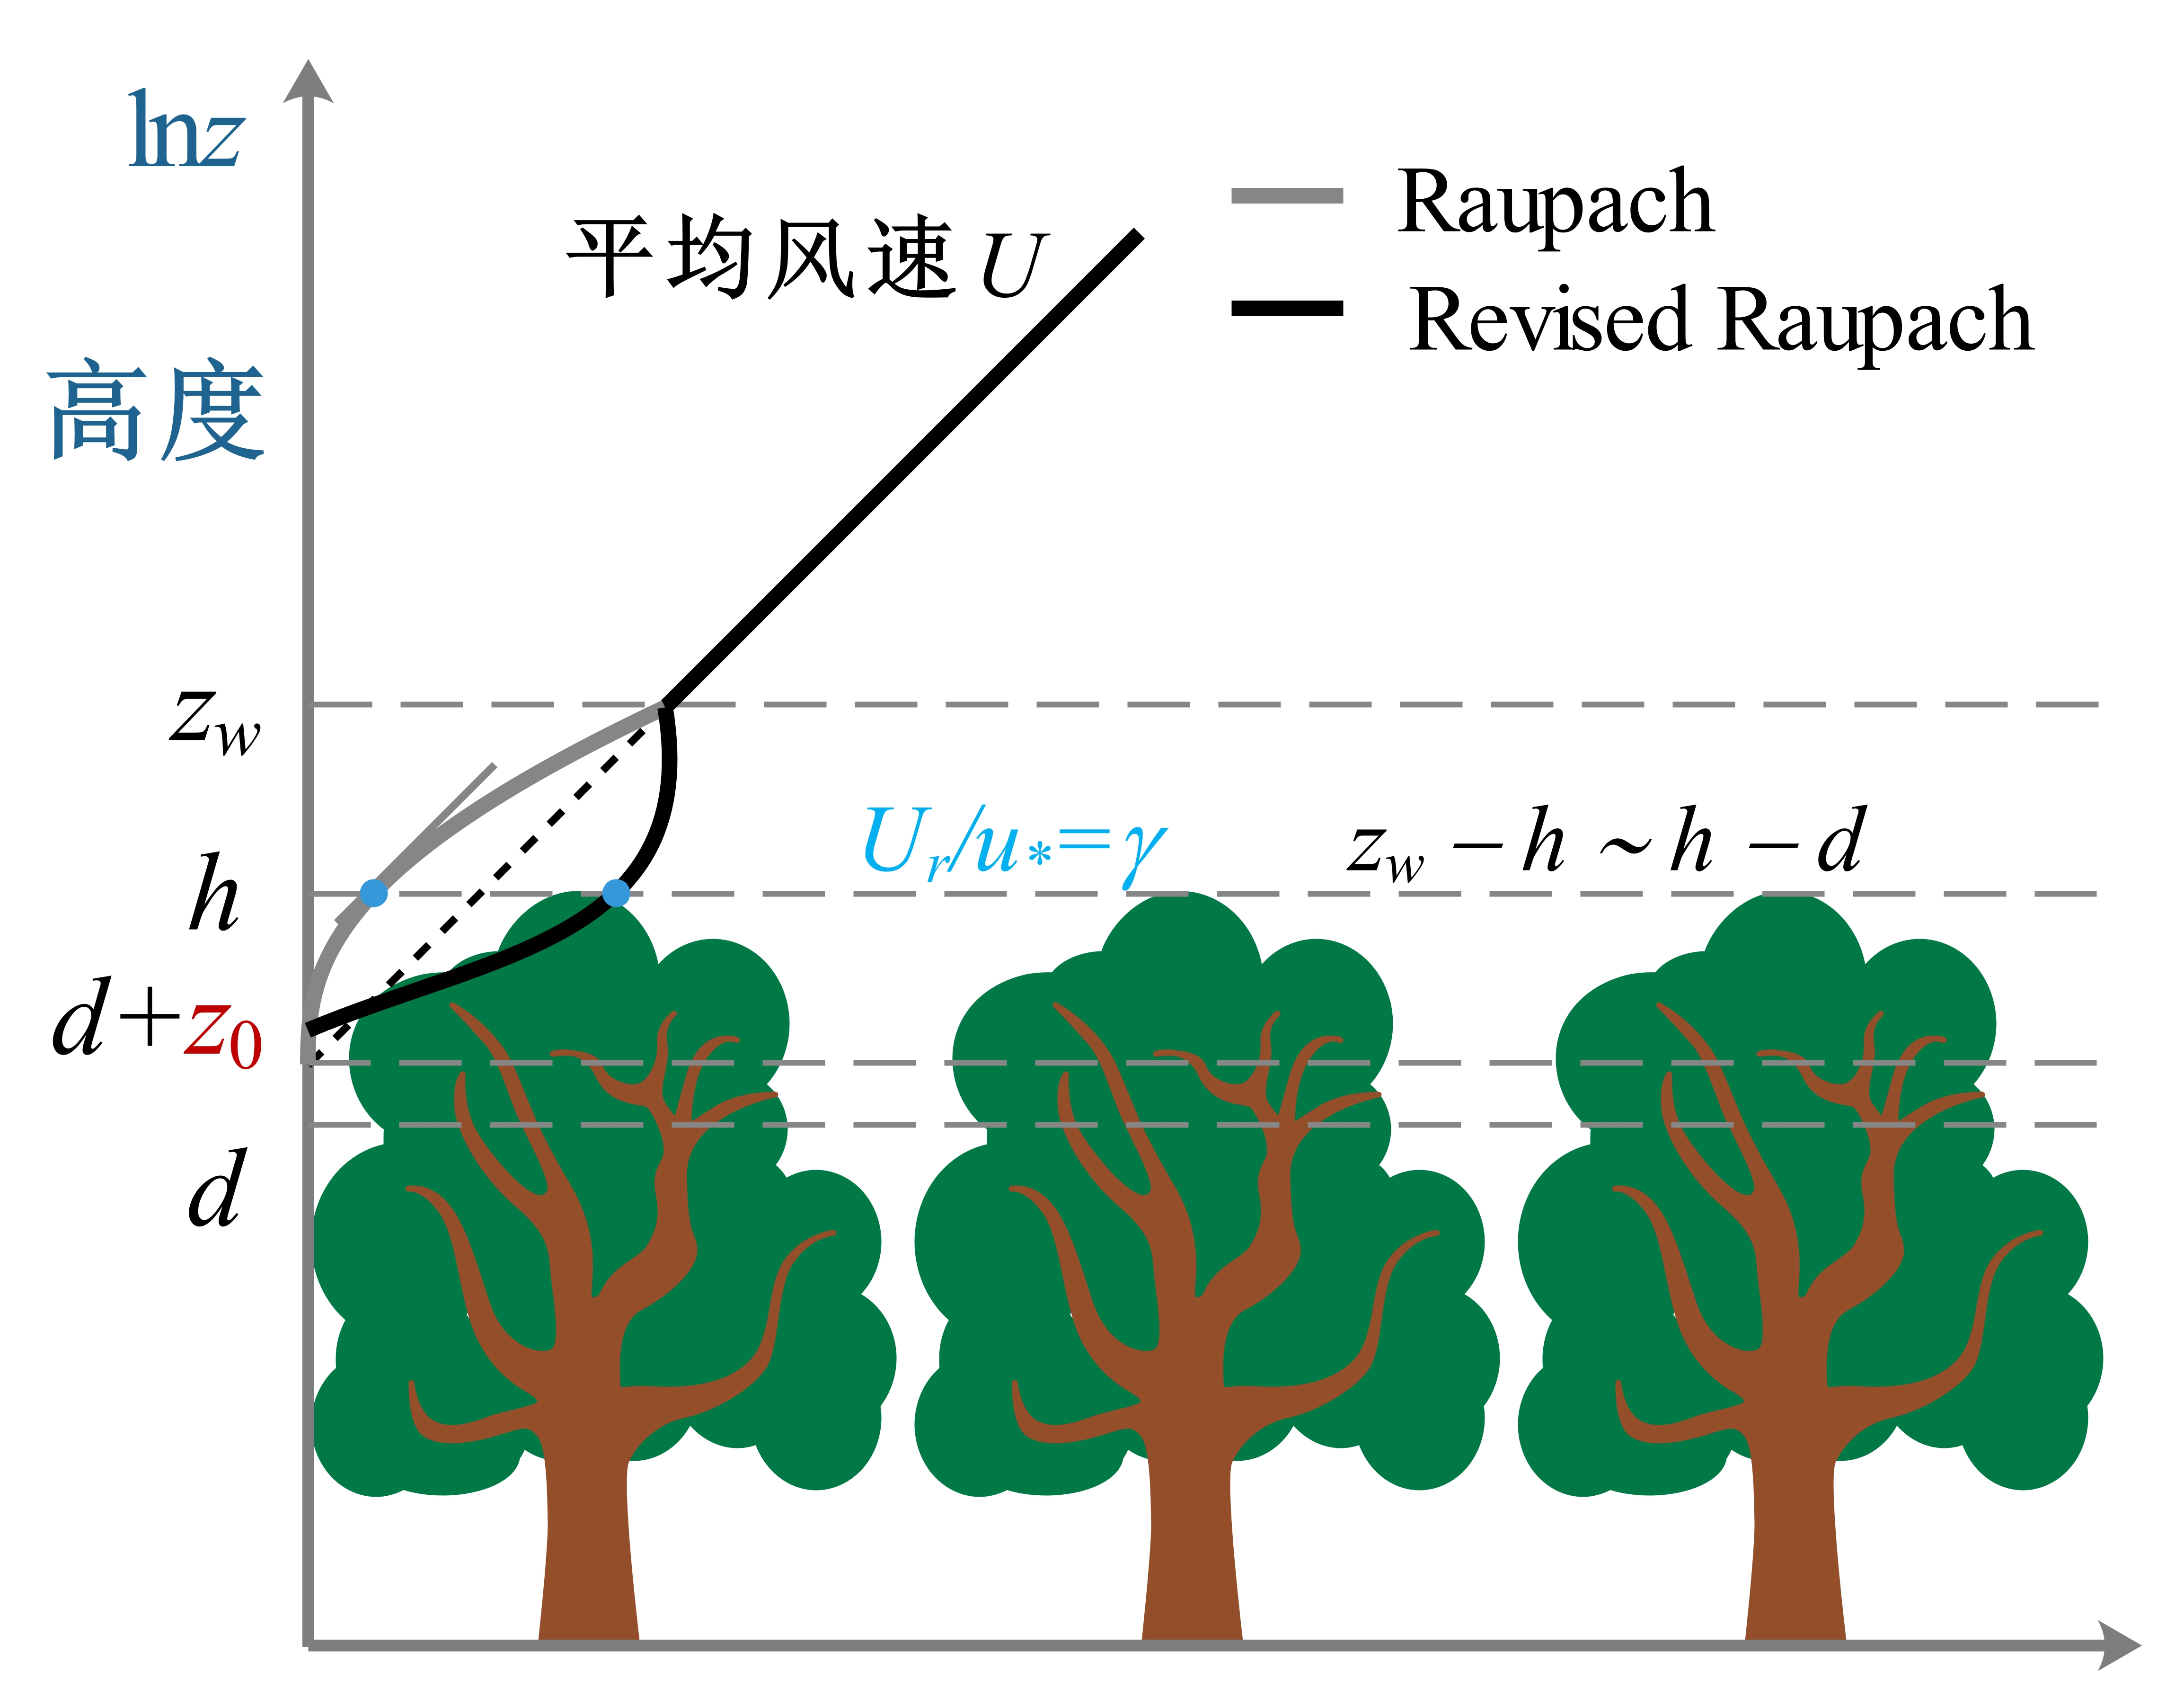
\includegraphics[scale=0.7]{Figures/地表湍流交换过程/修正Raupach粗糙度方案示意图.jpg}
    \caption{考虑稳定度影响的植被粗糙度计算方案意图}
    \label{fig:修正Raupach粗糙度方案示意图}
  \end{figure}
}


\subsection{单层植被湍流交换}\label{单层植被湍流交换}
单层植被不同于100\%植被覆盖假设,而是考虑植被树冠之间可能存在空隙,
即植被树冠存在一定的水平分布,树冠覆盖度可介于0$\sim$100\%之间。这种植被结果假设与三维植被辐射模型假设一致。


对于植被树冠稀疏覆盖时,\citet{raupach1992drag,raupach1994simplified}通过场外和风洞实验,发展了一套用于计算$z_0$和$d$的解析解,其中:
\begin{equation}\label{dooh0}
  \frac{d}{h}=1-\frac{1-\exp \left(-\sqrt{c_{\mathrm{d1}} 2 \lambda}\right)}{\sqrt{c_{\mathrm{d1}} 2 \lambda}}
\end{equation}
其中$c_{\mathrm{d1}}=7.5$,$\lambda$%表示植被迎风面积指数 ($FAI$),
计算为$f_{\mathrm {c}}\left[1-\exp{\left(-0.5\text{(LAI+SAI)}\right)}\right]$。
当植被覆盖$f_{\mathrm {c}}$等于100\%时,$\lambda$计算同100\%植被覆盖情景。为了同时适用于稀疏和浓密覆盖植被,
本版本采用~\citet{dai2019different}方案计算$d$:
\begin{equation}\label{dooh}
  \frac{d}{h}=f_{\mathrm{c}} \cdot 1.1 \ln \left(1+\left(c_{\mathrm{d}} f_{\mathrm{c}} \text{LAI}\right)^{0.25}\right)+\left(1-f_{\mathrm{c}}\right) \cdot\left(1-\frac{1-\exp \left(-\sqrt{c_{\mathrm{d1}} 2 \lambda}\right)}{\sqrt{c_{\mathrm{d1}} 2 \lambda}}\right)
\end{equation}
$z_0$的计算同公式 (\ref{zOh})。从上式可以看出,$d$值是100\%植被覆盖情景和稀疏植被按照植被覆盖度$f_{\mathrm {c}}$的加权平均,
当$f_{\mathrm {c}}\rightarrow100\%$时,公式 (\ref{dooh}) 趋同于公式 (\ref{dOh});当$f_{\mathrm {c}}\rightarrow0\%$时,趋同于公式 (\ref{dooh0})。


对于植被冠层内的风速廓线$u$和湍流交换系数$K$,同样采用$f_{\mathrm {c}}$加权方式。$u$和$K$分别计算为:
\begin{equation}
  u(z)=f_{\mathrm{c}} \cdot \min \big(u_{\mathrm{\exp }}(z), u_{\mathrm{comb}}(z)\big)+\left(1-f_{\mathrm{c}}\right) \cdot u_{\mathrm{comb}}
\end{equation}
\begin{equation}
  \frac{1}{K(z)}=f_{\mathrm{c}} \cdot \frac{1}{\min \big(K_{\mathrm{\exp}}(z), K_{\mathrm{comb}}(z)\big)}+\left(1-f_{\mathrm{c}}\right) \cdot \frac{1}{K_{\mathrm{comb}}}
\end{equation}
$u_{\mathrm{comb}}$和$K_{\mathrm{comb}}$同公式 (\ref{ucomb}) 和 (\ref{kcomb})。


当一层植被有多个PFT类型覆盖时,对于感热通量有平衡方程:
\begin{equation}
  H = H_{\mathrm g} + \sum_{i \in \mbox{\tiny {第1层}}}^{}H_{\mathrm{v}i}
\end{equation}
其中:
\begin{equation}
  H = \frac{\rho_{\mathrm{a}}C_{\mathrm{a}}\left( T_{1} - T_{\mathrm{a}} \right)}{r_{\mathrm{ah}}}
\end{equation}
%
\begin{equation}
  H_{\mathrm{g}} = \frac{\rho_{\mathrm{a}}C_{\mathrm{a}}\left( T_{\mathrm{g}} - T_{1} \right)}{r_{\mathrm{d1}}}
\end{equation}
%
\begin{equation}\label{eq:Hv_1L}
  H_{\mathrm{v}i} = \frac{\rho_{\mathrm{a}}C_{\mathrm{a}}f_{\mathrm{c}i}\left( T_{\mathrm{v}i} - T_{1} \right)}{r_{\mathrm{vh}i}}
\end{equation}
即:
\begin{equation}\label{eq:H_1L}
  \frac{\rho_{\mathrm{a}}C_{\mathrm{a}}\left( T_{1} - T_{\mathrm{a}} \right)}{r_{\mathrm{ah}}} = \frac{\rho_{\mathrm{a}}C_{\mathrm{a}}\left( T_{\mathrm{g}} - T_{1} \right)}{r_{\mathrm{d1}}} + \sum_{i \in \mbox{\tiny {第1层}}}^{}\frac{\rho_{\mathrm{a}}C_{\mathrm{a}}f_{\mathrm{c}i}\left( T_{\mathrm{v}i} - T_{1} \right)}{r_{\mathrm{vh}i}}
\end{equation}
%
上式中\(r_{\mathrm{ah}},r_{\mathrm{d1}},r_{\mathrm{vh}i}\)第一层等效交换高度到大气参考高度、地面和植被之间的感热交换阻抗,$r_{\mathrm{vh}i}$下标$i$表示不同PFT。令:
\begin{equation}
  c_{\mathrm{ah1}} = \frac{1}{r_{\mathrm{ah}}},\ c_{\mathrm{gh1}} = \frac{1}{r_{\mathrm{d1}}},\ c_{\mathrm{vh}i} = \frac{1}{r_{\mathrm{vh}i}}
\end{equation}
%
\begin{equation}
  w_{\mathrm{h1}} = c_{\mathrm{ah1}} + c_{\mathrm{gh1}} + \sum_{i \in \mbox{\tiny {第1层}}}^{}{f_{\mathrm{c}i}c_{\mathrm{vh}i}}
\end{equation}
%
\begin{equation}
  w_{\mathrm{ah1}} = \frac{c_{\mathrm{ah1}}}{w_{\mathrm{h1}}},\ w_{\mathrm{gh1}} = \frac{c_{\mathrm{gh1}}}{w_{\mathrm{h1}}},\ w_{\mathrm{vh}i} = \frac{f_{\mathrm{c}i}c_{\mathrm{vh}i}}{w_{\mathrm{h1}}}
\end{equation}
%
方程~\eqref{eq:H_1L} 进行变量替换,化简后可得:
\begin{equation}
  T_{1} = w_{\mathrm{ah1}}T_{\mathrm{a}} + w_{\mathrm{gh1}}T_{\mathrm{g}} + \sum_{i \in \mbox{\tiny {第1层}}}^{}{w_{\mathrm{vh}i}T_{\mathrm{v}i}}
\end{equation}
%
将上式\(T_{1}\)表达式带入到公式~\eqref{eq:Hv_1L} 中,即可计算叶片感热通量。叶片感热相对叶温变化的导数计算为:
\begin{equation}
  \frac{\partial H_{\mathrm{v}i}}{\partial T_{\mathrm{v}i}} = \rho_{\mathrm{a}}C_{\mathrm{a}}c_{\mathrm{vh}i}\left( 1 - w_{\mathrm{vh}i} \right)
\end{equation}
%
地面感热相对温度变化的导数为:
\begin{equation}
  \frac{\partial H_{\mathrm{g}}}{\partial T_{\mathrm{g}}} = \rho_{\mathrm{a}}C_{\mathrm{a}}c_{\mathrm{gh1}}\left( 1 - w_{\mathrm{gh1}} \right)
\end{equation}

对于潜热通量:
\begin{equation}
  \lambda E = {\lambda E}_{\mathrm{g}} + \sum_{i \in \mbox{\tiny {第1层}}}^{}{\lambda E}_{\mathrm{v}i}
\end{equation}
%
其中:
\begin{equation}
  E = \frac{\rho_{\mathrm{a}}\left( q_{1} - q_{\mathrm{a}} \right)}{r_{\mathrm{aw}}}
\end{equation}
%
\begin{equation}
  E_{\mathrm{g}} = \frac{\rho_{\mathrm{a}}\left( q_{\mathrm{g}} - q_{1} \right)}{r_{\mathrm{d1}}}
\end{equation}
%
\begin{equation}
  E_{\mathrm{v}i} = \frac{\rho_{\mathrm{a}}f_{\mathrm{c}i}\left( q_{\mathrm{v}i} - q_{1} \right)}{r_{\mathrm{vw}i}}
\end{equation}
%
即:
\begin{equation}\label{eq:LE_1L}
  \frac{\rho_{\mathrm{a}}\left( q_{1} - q_{\mathrm{a}} \right)}{r_{\mathrm{aw}}} = \frac{\rho_{\mathrm{a}}\left( q_{\mathrm{g}} - q_{1} \right)}{r_{\mathrm{d1}}} + \sum_{i \in \mbox{\tiny {第1层}}}^{}\frac{\rho_{\mathrm{a}}f_{\mathrm{c}i}\left( q_{\mathrm{v}i} - q_{1} \right)}{r_{\mathrm{vw}i}}
\end{equation}
%
上式中\(r_{\mathrm{aw}},r_{\mathrm{d1}},r_{\mathrm{vw}i}\)表示等效交换高度到大气参考高度、地面和植被之间的潜热交换阻抗。$q_{\mathrm{v}i}$表示叶片表面水汽比湿,为叶片温度$T_{\mathrm{v}i}$时的饱和比湿$q_{\mathrm{sat}}^{T_{\mathrm{v}i}}$。令:
\begin{equation}
  c_{\mathrm{aw1}} = \frac{1}{r_{\mathrm{aw}}},\ c_{\mathrm{gw1}} = \frac{1}{r_{\mathrm{d1}}},\ c_{\mathrm{vh}i} = \frac{1}{r_{\mathrm{vw}i}}
\end{equation}
%
\begin{equation}
  w_{\mathrm{q1}} = c_{\mathrm{aw1}} + c_{\mathrm{gw1}} + \sum_{i \in \mbox{\tiny {第1层}}}^{}{f_{\mathrm{c}i}c_{\mathrm{vw}i}}
\end{equation}
%
\begin{equation}
  w_{\mathrm{aq1}} = \frac{c_{\mathrm{aw1}}}{w_{\mathrm{q1}}},\ w_{\mathrm{gq1}} = \frac{c_{\mathrm{gw1}}}{w_{\mathrm{q1}}},\ w_{\mathrm{vq}i} = \frac{{f_{\mathrm{c}i}c}_{\mathrm{vw}i}}{w_{\mathrm{q}}}
\end{equation}
%
求解方程~\eqref{eq:LE_1L} 可得:
\begin{equation}
  q_{1} = w_{\mathrm{aw1}}q_{\mathrm{a}} + w_{\mathrm{gw1}}q_{\mathrm{g}} + \sum_{i \in \mbox{\tiny {第1层}}}^{}{w_{\mathrm{vq}i}q_{\mathrm{v}i}}
\end{equation}
%
叶片蒸散发相对叶温变化的导数计算为:
\begin{equation}
  \frac{\partial E_{\mathrm{v}i}}{\partial T_{\mathrm{v}i}} = \rho_{\mathrm{a}}c_{\mathrm{vw}i}\left( 1 - w_{\mathrm{vq}i} \right)\frac{{\rm d}q_{\mathrm{sat}}^{T_{\mathrm{v}i}}}{{\rm d}T_{\mathrm{v}i}}
\end{equation}
%
其中叶片蒸腾水汽通量相对叶片温度变化的导数计算为:
\begin{equation}
  \frac{\partial E_{\mathrm{vt}i}}{\partial T_{\mathrm{v}i}} = \rho_{\mathrm{a}}\left( 1 - f_{\mathrm{wet}} \right)\delta\left( \frac{\text{LAI}_{\mathrm{sun}}}{r_{\mathrm{b}i} + r_{\mathrm{s}i,\mathrm{sun}}} + \frac{\text{LAI}_{\mathrm{sha}}}{r_{\mathrm{b}i} + r_{\mathrm{s}i,sha}} \right)\left( 1 - w_{\mathrm{vq}i} \right)\frac{{\rm d}q_{\mathrm{sat}}^{T_{\mathrm{v}i}}}{{\rm d}T_{\mathrm{v}i}}
\end{equation}
%
叶片蒸发水汽通量相对叶片温度变化导数计算为:
\begin{equation}
  \frac{\partial E_{\mathrm{va}i}}{\partial T_{\mathrm{v}i}} = \rho_{\mathrm{a}}\left( 1 - \delta\left( 1 - f_{\mathrm{wet}} \right) \right)\frac{\text{LAI} + \text{SAI}}{r_{\mathrm{b}i}}\left( 1 - w_{\mathrm{vq}i} \right)\frac{{\rm d}q_{\mathrm{sat}}^{T_{\mathrm{v}i}}}{{\rm d}T_{\mathrm{v}i}}
\end{equation}
%
地面水汽通量相对温度变化的导数为:
\begin{equation}
  \frac{\partial E_{\mathrm{g}}}{\partial T_{\mathrm{g}}} = \rho_{\mathrm{a}}c_{\mathrm{gw1}}\left( 1 - w_{\mathrm{gq1}} \right)\frac{{\rm d}q_{\mathrm{g}}}{{\rm d}T_{\mathrm{g}}}
\end{equation}


\subsection{多层植被湍流交换}\label{多层植被湍流交换}
{
  \begin{figure}[htbp]
    \centering
    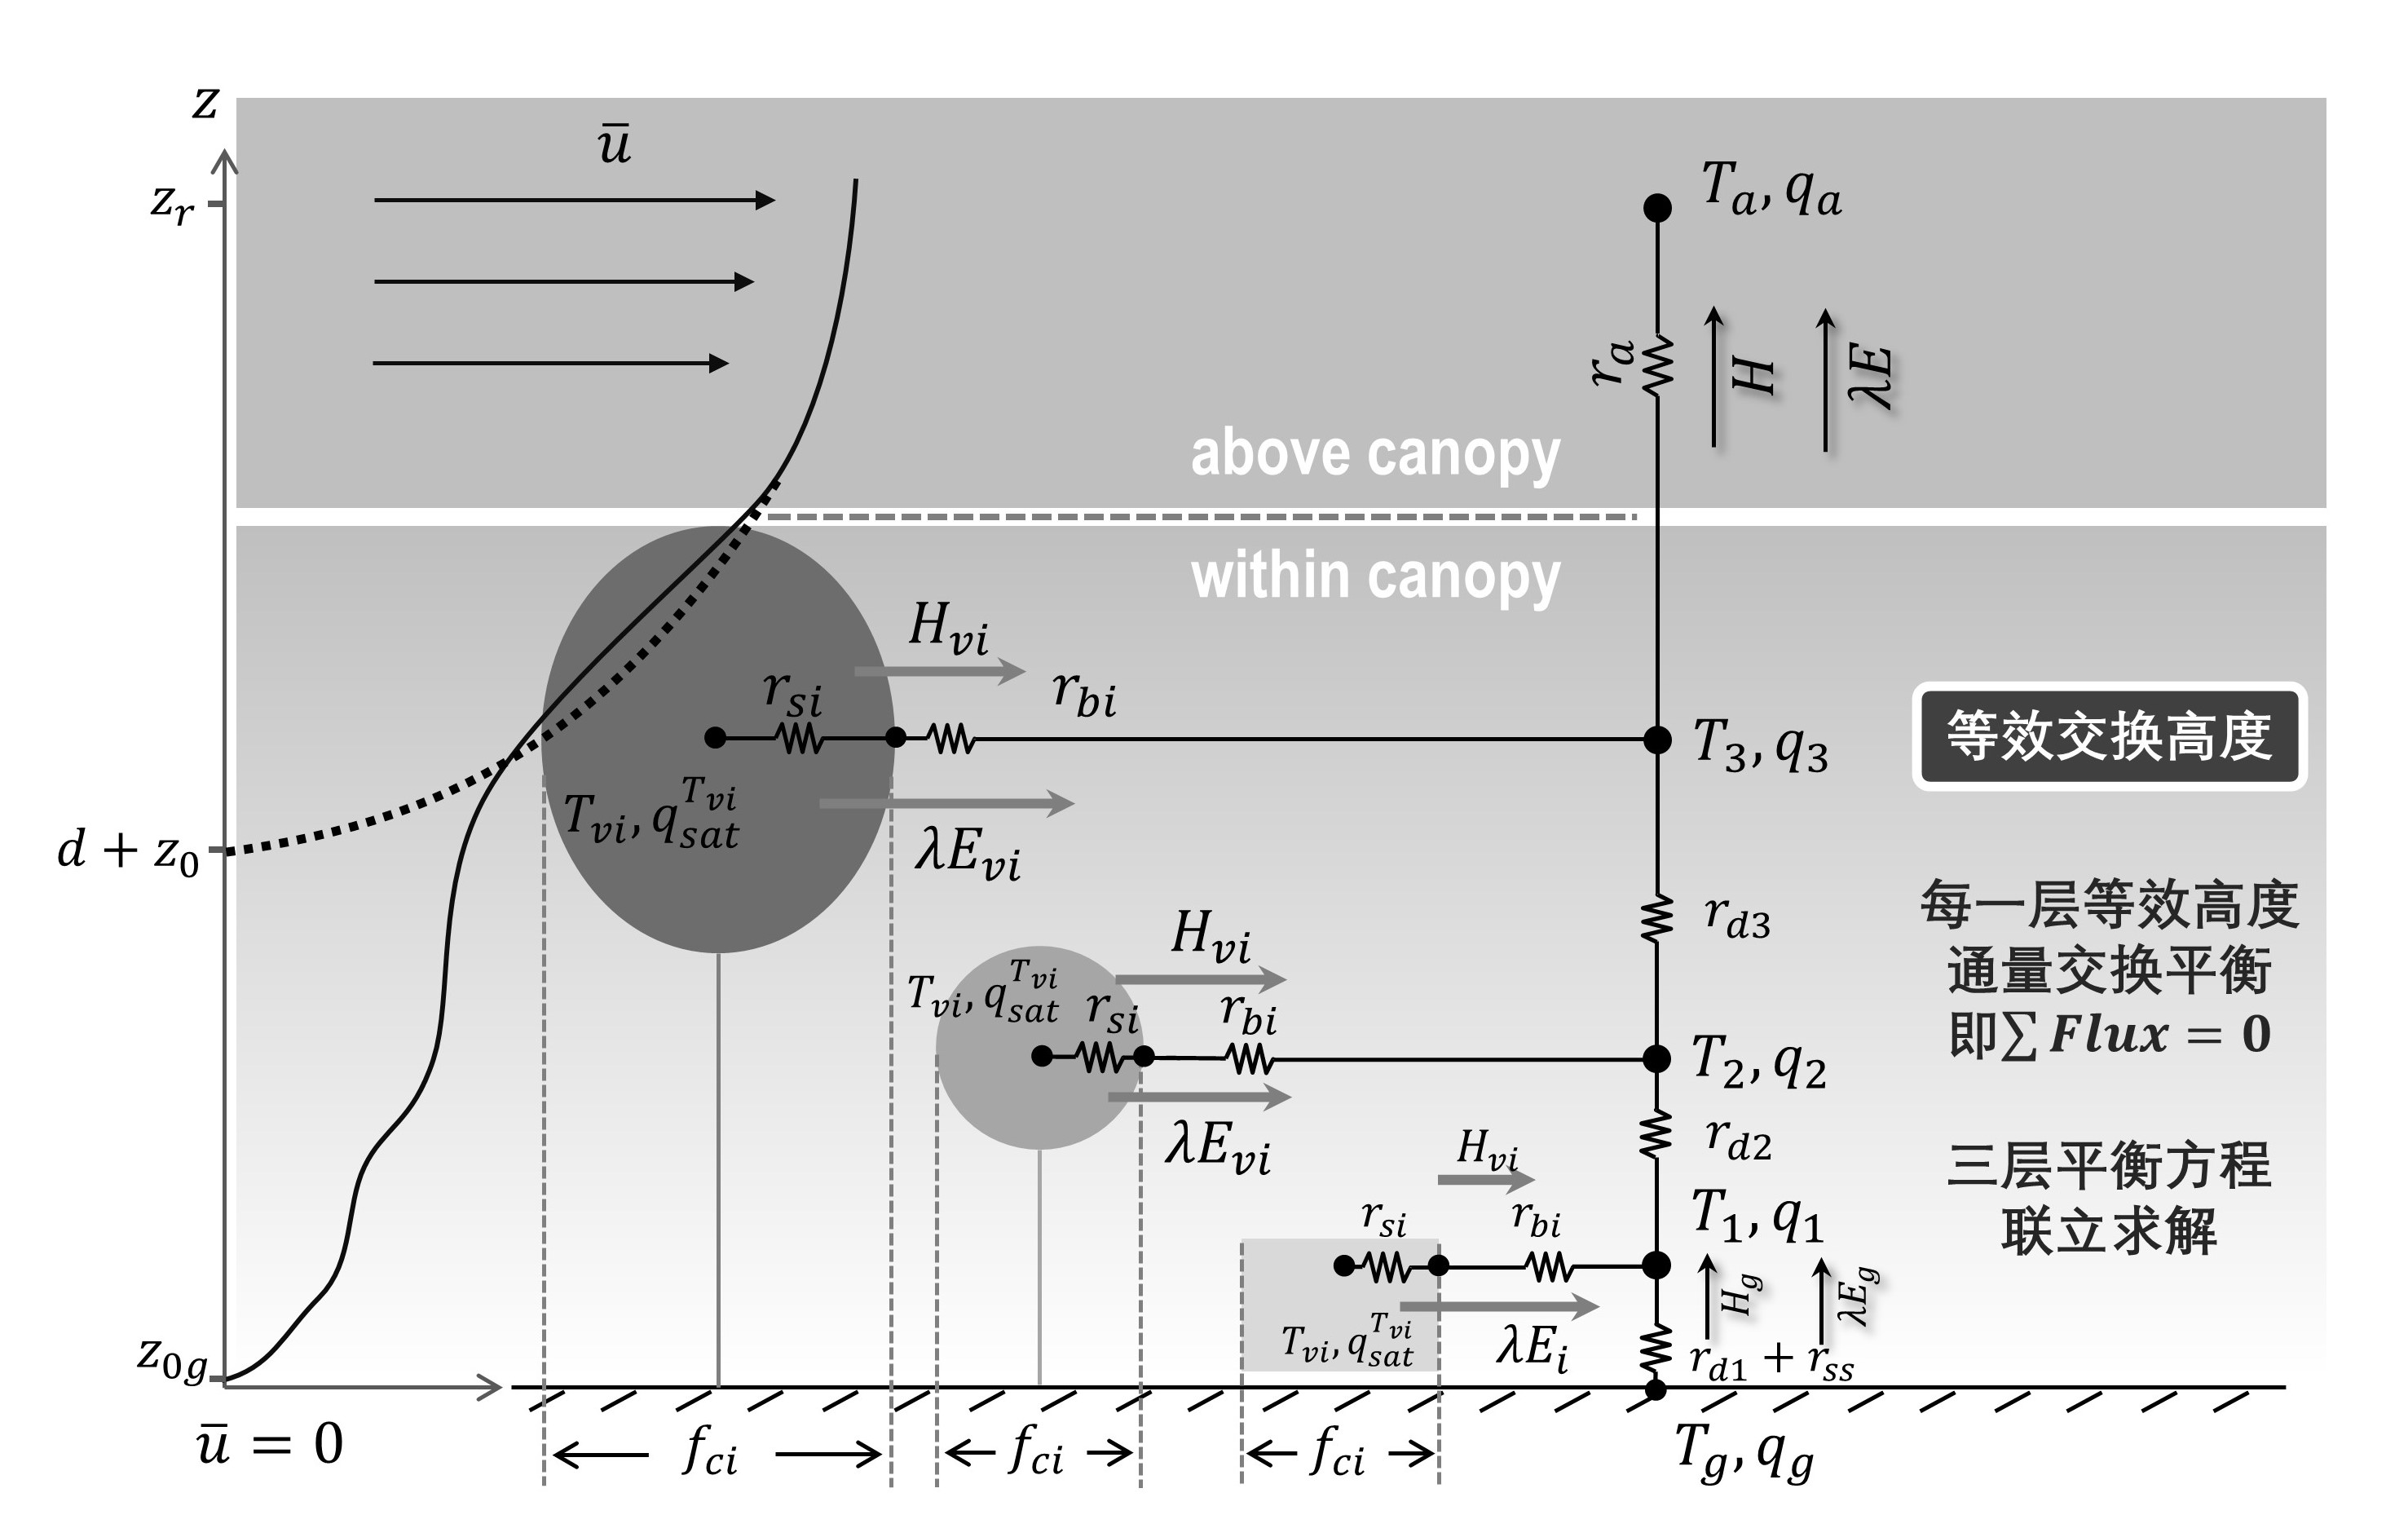
\includegraphics[width=1\linewidth]{Figures/地表湍流交换过程/三层植被湍流交换示意图_v3.jpg}
    \caption{三层植被湍流交换示意图}
    \label{fig:三层植被湍流交换示意图}
  \end{figure}
}

多层植被湍流计算是以单层植被计算为基础,总体阻抗网络如图~\ref{fig:三层植被湍流交换示意图} 所示。
风速$u$和湍流交换系数$K$廓线从最上层植被往下进行计算。上一层底部的廓线值作为下层植被顶部的值。
$r_{\mathrm {b}}$和$r_{\mathrm {d}}$的计算都是对$u$和$K$廓线的积分。
但积分区间对应到每层植被的等效交换高度(图~\ref{fig:三层植被湍流交换示意图} 中$T_{1}$、$T_{2}$、$T_{3}$位置所示)。
该交换高度计算为该层植被100\%覆盖时的$d+z_0$值。在每一层等效交换高度,建立通量(感热$H$和潜热$\lambda E$)平衡方程,即该点与上层通量交换量等于下层交换量加上该层植被的通量交换量。联立每层在等效高度建立的方程,迭代求解每种植被叶片温度。

通过以上介绍可以看出,三维植被湍流交换与一维植被湍流交换最大的不同在于其计算的对象由原来单一植被扩展到多种植被(PFT),并区分高度,因此阻抗网络发生较大变化,从而多种植被在同一物理环境下同时求解。在计算时,同一维植被一样,需要用到植被短波辐射吸收量和长波辐射吸收量,此时利用章节~\ref{三维植被辐射传输模型} 和 \ref{三维植被长波辐射传输} 对三维植被辐射传输计算结果,每种植被均采用双大叶模型模拟计算。整个植被冠层与大气的湍流交换同样采用相似性理论进行求解,其求解过程如图~\ref{fig:三维植被湍流交换模型计算流程图} 所示。
{
  \begin{figure}[htbp]
    \centering
    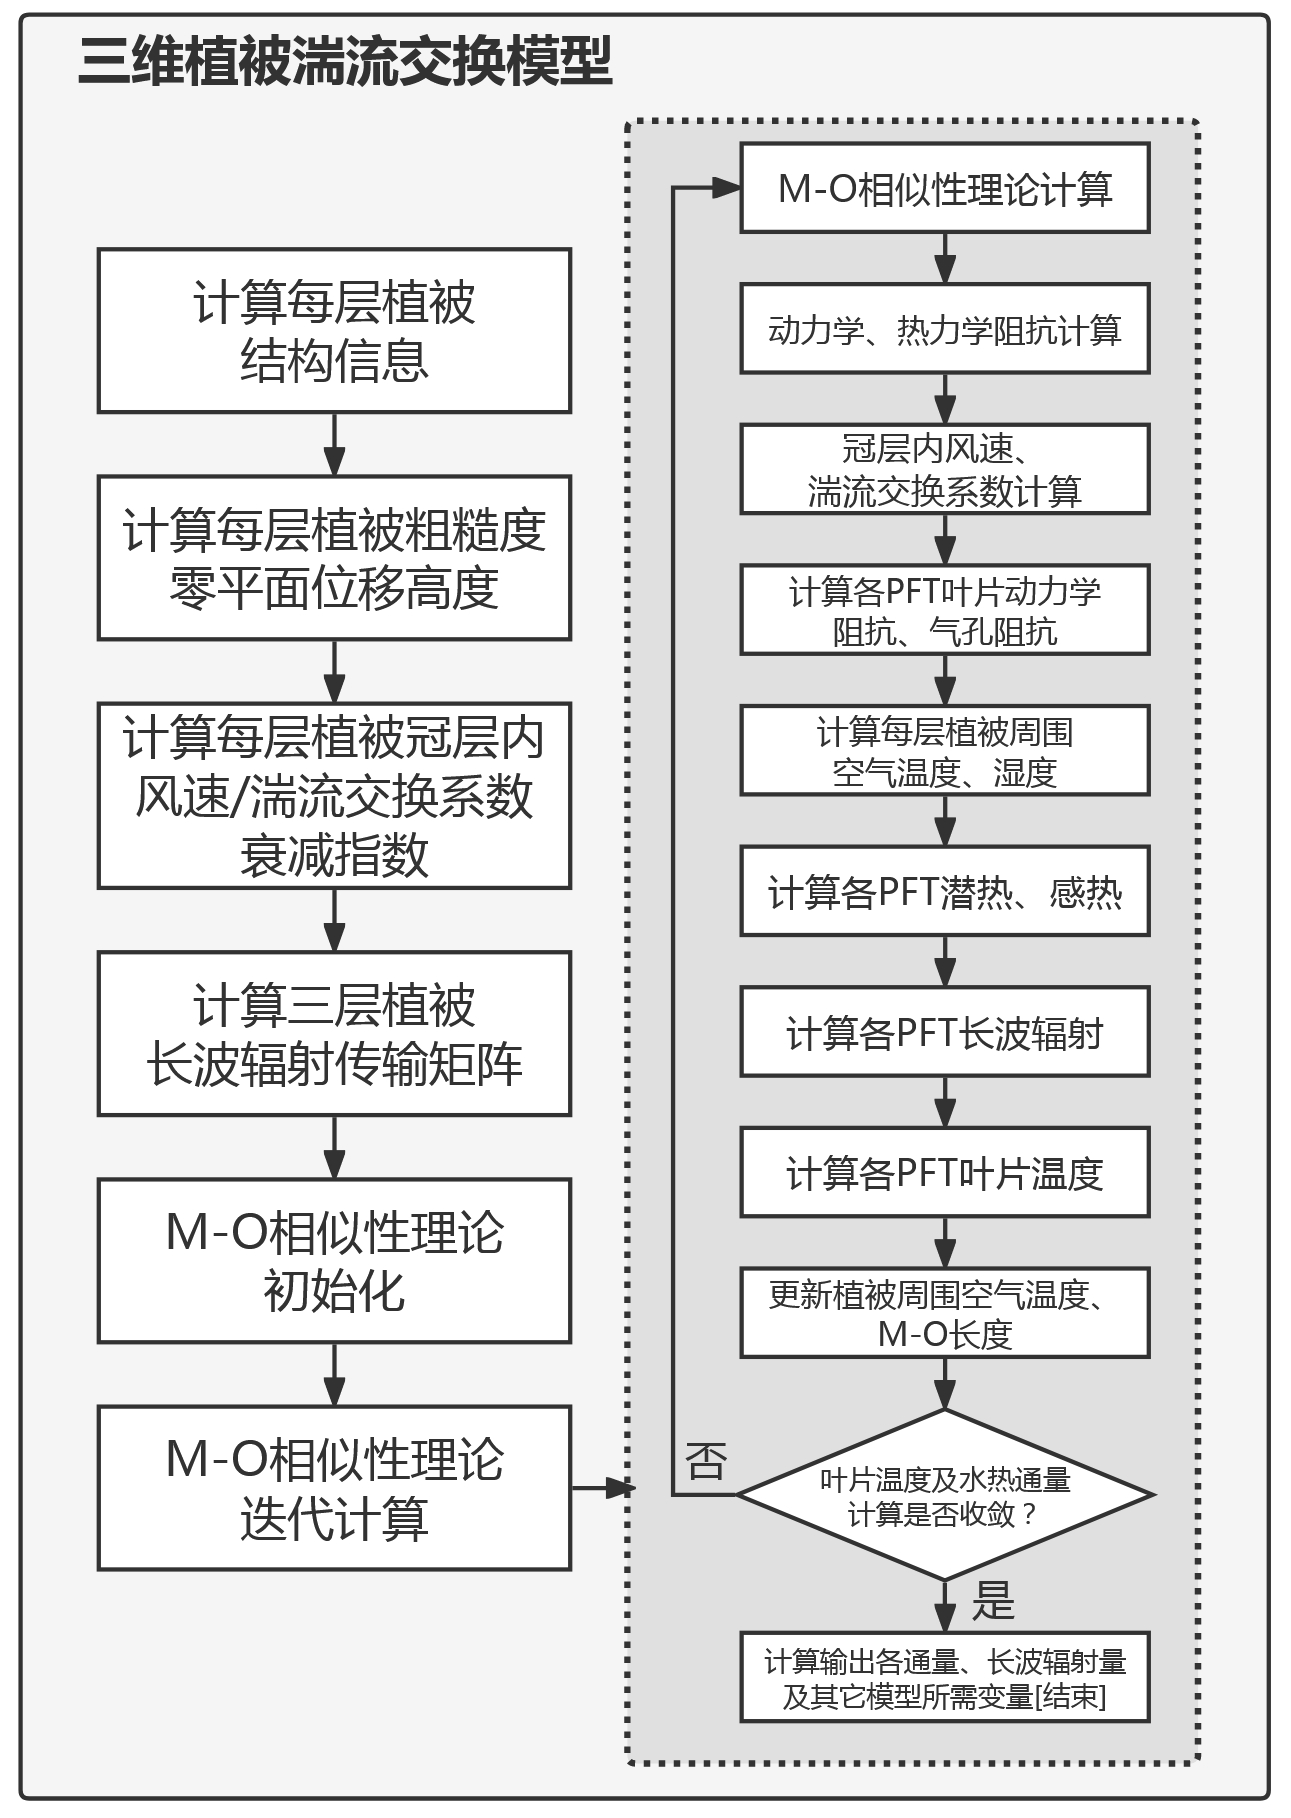
\includegraphics[width=0.75\linewidth]{Figures/地表湍流交换过程/三维植被湍流交换模型计算流程图_v2.png}
    \caption{三维植被湍流交换模型计算流程图}
    \label{fig:三维植被湍流交换模型计算流程图}
  \end{figure}
}


\subsubsection{两层植被}

当有两层植被覆盖时(较高层记为第2层,低层记为第1层),对与感热通量平衡方程为:
\begin{equation}
  H = H_{1} + \sum_{i \in \mbox{\tiny {第2层}}}^{}H_{\mathrm{v}i}
\end{equation}
%
\begin{equation}
  H_{1} = H_{\mathrm{g}} + \sum_{i \in \mbox{\tiny {第1层}}}^{}H_{\mathrm{v}i}
\end{equation}
%
即:
\begin{equation}\label{eq:H_2L_1}
  \frac{\rho_{\mathrm{a}}C_{\mathrm{a}}\left( T_{2} - T_{\mathrm{a}} \right)}{r_{\mathrm{ah}}} = \frac{\rho_{\mathrm{a}}C_{\mathrm{a}}\left( T_{1} - T_{2} \right)}{r_{\mathrm{d2}}} + \sum_{i \in \mbox{\tiny {第2层}}}^{}\frac{\rho_{\mathrm{a}}C_{\mathrm{a}}f_{\mathrm{c}i}\left( T_{\mathrm{v}i} - T_{2} \right)}{r_{\mathrm{vh}i}}
\end{equation}
%
\begin{equation}\label{eq:H_2L_2}
  \frac{\rho_{\mathrm{a}}C_{\mathrm{a}}\left( T_{1} - T_{2} \right)}{r_{\mathrm{d2}}} = \frac{\rho_{\mathrm{a}}C_{\mathrm{a}}\left( T_{\mathrm{g}} - T_{1} \right)}{r_{\mathrm{d1}}} + \sum_{i \in \mbox{\tiny {第1层}}}^{}\frac{\rho_{\mathrm{a}}C_{\mathrm{a}}f_{\mathrm{c}i}\left( T_{\mathrm{v}i} - T_{1} \right)}{r_{\mathrm{vh}i}}
\end{equation}
%
对于第2层方程,令:
\begin{equation}
  c_{\mathrm{ah2}} = \frac{1}{r_{\mathrm{ah}}},\ c_{\mathrm{gh2}} = \frac{1}{r_{\mathrm{d2}}},\ c_{\mathrm{vh}i} = \frac{1}{r_{\mathrm{vh}i}}
\end{equation}
%
\begin{equation}
  w_{\mathrm{h2}} = c_{\mathrm{ah2}} + c_{\mathrm{gh2}} + \sum_{i \in \mbox{\tiny {第2层}}}^{}{f_{\mathrm{c}i}c}_{\mathrm{vh}i}
\end{equation}
%
\begin{equation}
  w_{\mathrm{ah2}} = \frac{c_{\mathrm{ah2}}}{w_{\mathrm{h2}}},\ w_{\mathrm{gh2}} = \frac{c_{\mathrm{gh2}}}{w_{\mathrm{h2}}},\ w_{\mathrm{vh}i} = \frac{f_{\mathrm{c}i}c_{\mathrm{vh}i}}{w_{\mathrm{h2}}}
\end{equation}
%
对于第1层方程,令:
\begin{equation}
  c_{\mathrm{ah1}} = \frac{1}{r_{\mathrm{d2}}},\ c_{\mathrm{gh1}} = \frac{1}{r_{\mathrm{d1}}},\ c_{\mathrm{vh}i} = \frac{1}{r_{\mathrm{vh}i}}
\end{equation}
%
\begin{equation}
  w_{\mathrm{h1}} = c_{\mathrm{ah1}} + c_{\mathrm{gh1}} + \sum_{i \in \mbox{\tiny {第1层}}}^{}{f_{\mathrm{c}i}c}_{\mathrm{vh}i}
\end{equation}
%
\begin{equation}
  w_{\mathrm{ah1}} = \frac{c_{\mathrm{ah1}}}{w_{\mathrm{h1}}},\ w_{\mathrm{gh1}} = \frac{c_{\mathrm{gh1}}}{w_{\mathrm{h1}}},\ w_{\mathrm{vh}i} = \frac{{f_{\mathrm{c}i}c}_{\mathrm{vh}i}}{w_{\mathrm{h1}}}
\end{equation}
%
将方程~\eqref{eq:H_2L_2}得到的\(T_{1}\)表达式带入到方程~\eqref{eq:H_2L_1},即可求解\(T_{2}\)为:
\begin{equation}
  T_{2} = \frac{w_{\mathrm{ah2}}T_{\mathrm{a}} + w_{\mathrm{gh2}}T_{\mathrm{gv}} + \sum_{i \in \mbox{\tiny {第2层}}}^{}{w_{\mathrm{vh}i}T_{\mathrm{v}i}}}{f_{\mathrm{h}}}
\end{equation}
%
其中:
\begin{equation}
  T_{\mathrm{gv}} = w_{\mathrm{gh1}}T_{\mathrm{g}} + \sum_{i \in \mbox{\tiny {第1层}}}^{}{w_{\mathrm{vh}i}T_{\mathrm{v}i}}
\end{equation}
%
\begin{equation}
  f_{\mathrm{h}} = 1 - w_{\mathrm{gh2}}w_{\mathrm{ah1}}
\end{equation}
%
将计算得到的\(T_{2}\)带入到方程~\eqref{eq:H_2L_2},即可计算出\(T_{1}\)为:
\begin{equation}
  T_{1} = w_{\mathrm{ah1}}T_{2} + w_{\mathrm{gh1}}T_{\mathrm{g}} + \sum_{i \in \mbox{\tiny {第1层}}}^{}{w_{\mathrm{vh}i}T_{\mathrm{v}i}}
\end{equation}
%
对于第2层植被感热相对温度的导数计算为:
\begin{equation}
  \frac{\partial H_{\mathrm{v}i}}{\partial T_{\mathrm{v}i}} = \rho_{\mathrm{a}}C_{\mathrm{a}}c_{\mathrm{vh}i}\left( 1 - \frac{w_{\mathrm{vh}i}}{f_{\mathrm{h}}} \right)
\end{equation}
%
对于第1层植被感热相对温度的导数计算为:
\begin{equation}
  \frac{\partial H_{\mathrm{v}i}}{\partial T_{\mathrm{v}i}} = \rho_{\mathrm{a}}C_{\mathrm{a}}c_{\mathrm{vh}i}\left( 1 - \frac{w_{\mathrm{ah1}}w_{\mathrm{gh2}}w_{\mathrm{vh}i}}{f_{\mathrm{h}}} - w_{\mathrm{vh}i} \right) = \rho_{\mathrm{a}}C_{\mathrm{a}}c_{\mathrm{vh}i}\left( 1 - \frac{w_{\mathrm{vh}i}}{f_{\mathrm{h}}} \right)
\end{equation}
%
地面感热相对温度变化的导数计算为:
\begin{equation}
  \frac{\partial H_{\mathrm{g}}}{\partial T_{\mathrm{g}}} = \rho_{\mathrm{a}}C_{\mathrm{a}}c_{\mathrm{gh1}}\left( 1 - \frac{w_{\mathrm{ah1}}w_{\mathrm{gh2}}w_{\mathrm{gh1}}}{f_{\mathrm h}} - w_{\mathrm{gh1}} \right) = \rho_{\mathrm{a}}C_{\mathrm{a}}c_{\mathrm{gh1}}\left( 1 - \frac{w_{\mathrm{gh1}}}{f_{\mathrm h}} \right)
\end{equation}


对于潜热通量:
\begin{equation}
  \lambda E = {\lambda E}_{1} + \sum_{i \in \mbox{\tiny {第2层}}}^{}{\lambda E_{\mathrm{v}i}}
\end{equation}
%
\begin{equation}
  {\lambda E}_{1} = \lambda E_{\mathrm{g}} + \sum_{i \in \mbox{\tiny {第1层}}}^{}{\lambda E_{\mathrm{v}i}}
\end{equation}
%
即:
\begin{equation}\label{eq:LE_2L_1}
  \frac{\rho_{\mathrm{a}}\left( q_{2} - q_{\mathrm{a}} \right)}{r_{\mathrm{aw}}} = \frac{\rho_{\mathrm{a}}\left( q_{1} - q_{2} \right)}{r_{\mathrm{d2}}} + \sum_{i \in \mbox{\tiny {第2层}}}^{}\frac{\rho_{\mathrm{a}}f_{\mathrm{c}i}\left( q_{\mathrm{v}i} - q_{2} \right)}{r_{\mathrm{vw}i}}
\end{equation}
%
\begin{equation}\label{eq:LE_2L_2}
  \frac{\rho_{\mathrm{a}}\left( q_{1} - q_{2} \right)}{r_{\mathrm{d2}}} = \frac{\rho_{\mathrm{a}}\left( q_{\mathrm{g}} - q_{1} \right)}{r_{\mathrm{d1}}} + \sum_{i \in \mbox{\tiny {第1层}}}^{}\frac{\rho_{\mathrm{a}}f_{\mathrm{c}i}\left( q_{\mathrm{v}i} - q_{1} \right)}{r_{\mathrm{vw}i}}
\end{equation}
%
对于第2层方程,令:
\begin{equation}
  c_{\mathrm{aw2}} = \frac{1}{r_{\mathrm{aw}}},\ c_{\mathrm{gw2}} = \frac{1}{r_{\mathrm{d2}}},\ c_{\mathrm{vw}i} = \frac{1}{r_{\mathrm{vw}i}}
\end{equation}
%
\begin{equation}
  w_{q2} = c_{\mathrm{aw2}} + c_{\mathrm{gw2}} + \sum_{i \in \mbox{\tiny {第2层}}}^{}{f_{\mathrm{c}i}\ c_{\mathrm{vw}i}}
\end{equation}
%
\begin{equation}
  w_{\mathrm{aq2}} = \frac{c_{\mathrm{aw2}}}{w_{\mathrm{q2}}},\ w_{\mathrm{gh2}} = \frac{c_{\mathrm{gw2}}}{w_{\mathrm{q2}}},\ w_{\mathrm{vh}i} = \frac{{f_{\mathrm{c}i}c}_{\mathrm{vw}i}}{w_{\mathrm{q2}}}
\end{equation}
%
对于第1层方程,令:
\begin{equation}
  c_{\mathrm{aw1}} = \frac{1}{r_{\mathrm{d2}}},\ c_{\mathrm{gw1}} = \frac{1}{r_{\mathrm{d1}}},\ c_{\mathrm{vw}i} = \frac{1}{r_{\mathrm{vw}i}}
\end{equation}
%
\begin{equation}
  w_{\mathrm{q1}} = c_{\mathrm{aw1}} + c_{\mathrm{gw1}} + \sum_{i \in \mbox{\tiny {第1层}}}^{}{f_{\mathrm{c}i}c}_{\mathrm{vw}i}
\end{equation}
%
\begin{equation}
  w_{\mathrm{aq1}} = \frac{c_{\mathrm{aw1}}}{w_{\mathrm{q1}}},\ w_{\mathrm{gq1}} = \frac{c_{\mathrm{gw1}}}{w_{\mathrm{q1}}},\ w_{\mathrm{vh}i} = \frac{{f_{\mathrm{c}i}c}_{\mathrm{vw}i}}{w_{\mathrm{q1}}}
\end{equation}
%
将方程~\eqref{eq:LE_2L_2} 得到的\(q_{1}\)表达式带入到方程~\eqref{eq:LE_2L_1},即可求解\(q_{2}\)为:
\begin{equation}
  q_{2} = \frac{w_{\mathrm{aq2}}q_{\mathrm{a}} + w_{\mathrm{gq2}}q_{\mathrm{gv}} + \sum_{i \in \mbox{\tiny {第2层}}}^{}{w_{\mathrm{vq}i}q_{\mathrm{v}i}}}{f_{\mathrm{q}}}
\end{equation}
%
其中:
\begin{equation}
  q_{\mathrm{gv}} = w_{\mathrm{gq1}}q_{\mathrm{g}} + \sum_{i \in \mbox{\tiny {第1层}}}^{}{w_{\mathrm{vq}i}q_{\mathrm{v}i}}
\end{equation}
%
\begin{equation}
  f_{\mathrm{q}} = 1 - w_{\mathrm{gq2}}w_{\mathrm{aq1}}
\end{equation}
%
将计算得到的\(q_{2}\)带入到方程~\eqref{eq:LE_2L_2},即可计算出\(q_{1}\)为:
\begin{equation}
  q_{1} = w_{\mathrm{aq1}}q_{2} + w_{\mathrm{gq1}}q_{\mathrm{g}} + \sum_{i \in \mbox{\tiny {第1层}}}^{}{w_{\mathrm{vq}i}q_{\mathrm{v}i}}
\end{equation}
%
第2层植被叶片蒸散发相对叶温变化的导数计算为:
\begin{equation}
  \frac{\partial E_{\mathrm{v}i}}{\partial T_{\mathrm{v}i}} = \rho_{\mathrm{a}}c_{\mathrm{vw}i}\left( 1 - \frac{w_{\mathrm{vq}i}}{f_{\mathrm{q}}} \right)\frac{{\rm d}q_{\mathrm{sat}}^{T_{\mathrm{v}i}}}{{\rm d}T_{\mathrm{v}i}}
\end{equation}
%
其中叶片蒸腾水汽通量相对叶片温度变化的导数计算为:
\begin{equation}
  \frac{\partial E_{\mathrm{vt}i}}{\partial T_{\mathrm{v}i}} = \rho_{\mathrm{a}}\left( 1 - f_{\mathrm{wet}} \right)\delta\left( \frac{\text{LAI}_{\mathrm{sun}}}{r_{\mathrm{b}i} + r_{\mathrm{s}i,\mathrm{sun}}} + \frac{\text{LAI}_{\mathrm{sha}}}{r_{\mathrm{b}i} + r_{\mathrm{s}i,sha}} \right)\left( 1 - \frac{w_{\mathrm{vq}i}}{f_{\mathrm{q}}} \right)\frac{{\rm d}q_{\mathrm{sat}}^{T_{\mathrm{v}i}}}{{\rm d}T_{\mathrm{v}i}}
\end{equation}
%
叶片蒸发水汽通量相对叶片温度变化导数计算为:
\begin{equation}
  \frac{\partial E_{\mathrm{va}i}}{\partial T_{\mathrm{v}i}} = \rho_{\mathrm{a}}\left( 1 - \delta\left( 1 - f_{\mathrm{wet}} \right) \right)\frac{\text{LAI} + \text{SAI}}{r_{\mathrm{b}i}}\left( 1 - \frac{w_{\mathrm{vq}i}}{f_{\mathrm{q}}} \right)\frac{{\rm d}q_{\mathrm{sat}}^{T_{\mathrm{v}i}}}{{\rm d}T_{\mathrm{v}i}}
\end{equation}
%
第1层植被叶片蒸散发相对叶温变化的导数计算为:
\begin{equation}
  \frac{\partial E_{\mathrm{v}i}}{\partial T_{\mathrm{v}i}} = \rho_{\mathrm{a}}c_{\mathrm{vw}i}\left( 1 - \frac{w_{\mathrm{vq}i}}{f_{\mathrm{q}}} \right)\frac{{\rm d}q_{\mathrm{sat}}^{T_{\mathrm{v}i}}}{{\rm d}T_{\mathrm{v}i}}
\end{equation}
%
其中叶片蒸腾水汽通量相对叶片温度变化的导数计算为:
\begin{equation}
  \frac{\partial E_{\mathrm{vt}i}}{\partial T_{\mathrm{v}i}} = \rho_{\mathrm{a}}\left( 1 - f_{\mathrm{wet}} \right)\delta\left( \frac{\text{LAI}_{\mathrm{sun}}}{r_{\mathrm{b}i} + r_{\mathrm{s}i,\mathrm{sun}}} + \frac{\text{LAI}_{\mathrm{sha}}}{r_{\mathrm{b}i} + r_{\mathrm{s}i,sha}} \right)\left( 1 - \frac{w_{\mathrm{vq}i}}{f_{\mathrm{q}}} \right)\frac{{\rm d}q_{\mathrm{sat}}^{T_{\mathrm{v}i}}}{{\rm d}T_{\mathrm{v}i}}
\end{equation}
%
叶片蒸发水汽通量相对叶片温度变化导数计算为:
\begin{equation}
  \frac{\partial E_{\mathrm{va}i}}{\partial T_{\mathrm{v}i}} = \rho_{\mathrm{a}}\left( 1 - \delta\left( 1 - f_{\mathrm{wet}} \right) \right)\frac{\text{LAI} + \text{SAI}}{r_{\mathrm{b}i}}\left( 1 - \frac{w_{\mathrm{vq}i}}{f_{\mathrm{q}}} \right)\frac{{\rm d}q_{\mathrm{sat}}^{T_{\mathrm{v}i}}}{{\rm d}T_{\mathrm{v}i}}
\end{equation}
%
地面水汽通量相对温度变化的导数为:
\begin{equation}
  \frac{\partial E_{\mathrm{g}}}{\partial T_{\mathrm{g}}} = \rho_{\mathrm{a}}c_{\mathrm{gw1}}\left( 1 - \frac{w_{\mathrm{gq1}}}{f_{\mathrm {q}}} \right)\frac{{\rm d}q_{\mathrm{g}}}{{\rm d}T_{\mathrm{g}}}
\end{equation}

\subsubsection{三层植被}

当为三层植被覆盖时,对于感热通量:
\begin{equation}
  H = H_{2} + \sum_{i \in \mbox{\tiny {第3层}}}^{}H_{\mathrm{v}i}
\end{equation}
%
\begin{equation}
  H_{2} = H_{1} + \sum_{i \in \mbox{\tiny {第2层}}}^{}H_{\mathrm{v}i}
\end{equation}
%
\begin{equation}
  H_{1} = H_{\mathrm{g}} + \sum_{i \in \mbox{\tiny {第1层}}}^{}H_{\mathrm{v}i}
\end{equation}
%
即:
\begin{equation}\label{eq:H_3L_1}
  \frac{\rho_{\mathrm{a}}C_{\mathrm{a}}\left( T_{3} - T_{\mathrm{a}} \right)}{r_{\mathrm{ah}}} = \frac{\rho_{\mathrm{a}}C_{\mathrm{a}}\left( T_{2} - T_{3} \right)}{r_{\mathrm{d3}}} + \sum_{i \in \mbox{\tiny {第3层}}}^{}\frac{\rho_{\mathrm{a}}C_{\mathrm{a}}f_{\mathrm{c}i}\left( T_{\mathrm{v}i} - T_{3} \right)}{r_{\mathrm{vh}i}}
\end{equation}
%
\begin{equation}\label{eq:H_3L_2}
  \frac{\rho_{\mathrm{a}}C_{\mathrm{a}}\left( T_{2} - T_{3} \right)}{r_{\mathrm{d3}}} = \frac{\rho_{\mathrm{a}}C_{\mathrm{a}}\left( T_{1} - T_{2} \right)}{r_{\mathrm{d2}}} + \sum_{i \in \mbox{\tiny {第2层}}}^{}\frac{\rho_{\mathrm{a}}C_{\mathrm{a}}f_{\mathrm{c}i}\left( T_{\mathrm{v}i} - T_{2} \right)}{r_{\mathrm{vh}i}}
\end{equation}
%
\begin{equation}\label{eq:H_3L_3}
  \frac{\rho_{\mathrm{a}}C_{\mathrm{a}}\left( T_{1} - T_{2} \right)}{r_{\mathrm{d2}}} = \frac{\rho_{\mathrm{a}}C_{\mathrm{a}}\left( T_{\mathrm{g}} - T_{1} \right)}{r_{\mathrm{d1}}} + \sum_{i \in \mbox{\tiny {第1层}}}^{}\frac{\rho_{\mathrm{a}}C_{\mathrm{a}}f_{\mathrm{c}i}\left( T_{\mathrm{v}i} - T_{1} \right)}{r_{\mathrm{vh}i}}
\end{equation}
%
对于第3层方程,令:
\begin{equation}
  c_{\mathrm{ah3}} = \frac{1}{r_{\mathrm{ah}}},\ c_{\mathrm{gh3}} = \frac{1}{r_{\mathrm{d3}}},\ c_{\mathrm{vh}i} = \frac{1}{r_{\mathrm{vh}i}}
\end{equation}
%
\begin{equation}
  w_{\mathrm{h3}} = c_{\mathrm{ah3}} + c_{\mathrm{gh3}} + \sum_{i \in \mbox{\tiny {第3层}}}^{}{f_{\mathrm{c}i}c_{\mathrm{vh}i}}
\end{equation}
%
\begin{equation}
  w_{\mathrm{ah3}} = \frac{c_{\mathrm{ah3}}}{w_{\mathrm{h3}}},\ w_{\mathrm{gh3}} = \frac{c_{\mathrm{gh3}}}{w_{\mathrm{h3}}},\ w_{\mathrm{vh}i} = \frac{f_{\mathrm{c}i}c_{\mathrm{vh}i}}{w_{\mathrm{h3}}}
\end{equation}
%
对于第2层方程,令:
\begin{equation}
  c_{\mathrm{ah2}} = \frac{1}{r_{\mathrm{d3}}},\ c_{\mathrm{gh2}} = \frac{1}{r_{\mathrm{d2}}},\ c_{\mathrm{vh}i} = \frac{1}{r_{\mathrm{vh}i}}
\end{equation}
%
\begin{equation}
  w_{\mathrm{h2}} = c_{\mathrm{ah2}} + c_{\mathrm{gh2}} + \sum_{i \in \mbox{\tiny {第2层}}}^{}{f_{\mathrm{c}i}c_{\mathrm{vh}i}}
\end{equation}
%
\begin{equation}
  w_{\mathrm{ah2}} = \frac{c_{\mathrm{ah2}}}{w_{\mathrm{h2}}},\ w_{\mathrm{gh2}} = \frac{c_{\mathrm{gh2}}}{w_{\mathrm{h2}}},\ w_{\mathrm{vh}i} = \frac{f_{\mathrm{c}i}c_{\mathrm{vh}i}}{w_{\mathrm{h2}}}
\end{equation}
%
对于第1层方程,令:
\begin{equation}
  c_{\mathrm{ah1}} = \frac{1}{r_{\mathrm{d2}}},\ c_{\mathrm{gh1}} = \frac{1}{r_{\mathrm{d1}}},\ c_{\mathrm{vh}i} = \frac{1}{r_{\mathrm{vh}i}}
\end{equation}
%
\begin{equation}
  w_{\mathrm{h1}} = c_{\mathrm{ah1}} + c_{\mathrm{gh1}} + \sum_{i \in \mbox{\tiny {第1层}}}^{}{f_{\mathrm{c}i}c_{\mathrm{vh}i}}
\end{equation}
%
\begin{equation}
  w_{\mathrm{ah1}} = \frac{c_{\mathrm{ah1}}}{w_{\mathrm{h1}}},\ w_{\mathrm{gh1}} = \frac{c_{\mathrm{gh1}}}{w_{\mathrm{h1}}},\ w_{\mathrm{vh}i} = \frac{f_{\mathrm{c}i}c_{\mathrm{vh}i}}{w_{\mathrm{h1}}}
\end{equation}
%
将方程~\eqref{eq:H_3L_1} 关于\(T_{3}\)的表达式和方程~\eqref{eq:H_3L_3}关于\(T_{1}\)的表达式带入方程~\eqref{eq:H_3L_2},可计算\(T_{2}\)为:
\begin{equation}
  T_{2} = \frac{w_{\mathrm{ah2}}T_{\mathrm{av}} + w_{\mathrm{gh2}}T_{\mathrm{gv}} + \sum_{i \in \mbox{\tiny {第二层}}}^{}{w_{\mathrm{vh}i}T_{\mathrm{v}i}}}{f_{\mathrm{h}}}
\end{equation}
%
其中:
\begin{equation}
  T_{\mathrm{av}} = w_{\mathrm{ah3}}T_{\mathrm{a}} + \sum_{i \in \mbox{\tiny {第3层}}}^{}{w_{\mathrm{vh}i}T_{\mathrm{v}i}}
\end{equation}
%
\begin{equation}
  T_{\mathrm{gv}} = w_{\mathrm{gh1}}T_{\mathrm{g}} + \sum_{i \in \mbox{\tiny {第1层}}}^{}{w_{\mathrm{vh}i}T_{\mathrm{v}i}}
\end{equation}
%
\begin{equation}
  f_{\mathrm{h}} = 1 - w_{\mathrm{ah2}}w_{\mathrm{gh3}} - w_{\mathrm{gh2}}w_{\mathrm{ah1}}
\end{equation}
%
将\(T_{2}\)表达式带入到方程中,即可得到\(T_{1}\)和\(T_{3}\)表达式:
\begin{equation}
  T_{1} = w_{\mathrm{ah1}}T_{\mathrm{2}} + w_{\mathrm{gh1}}T_{\mathrm{g}} + \sum_{i \in \mbox{\tiny {第1层}}}^{}{w_{\mathrm{vh}i}T_{\mathrm{v}i}}
\end{equation}
%
\begin{equation}
  T_{3} = w_{\mathrm{ah3}}T_{\mathrm{a}} + w_{\mathrm{gh3}}T_{2} + \sum_{i \in \mbox{\tiny {第3层}}}^{}{w_{\mathrm{vh}i}T_{\mathrm{v}i}}
\end{equation}
%
对于第2层植被感热相对温度的导数计算为:
\begin{equation}
  \frac{\partial H_{\mathrm{v}i}}{\partial T_{\mathrm{v}i}} = \rho_{\mathrm{a}}C_{\mathrm{a}}c_{\mathrm{vh}i}\left( 1 - \frac{w_{\mathrm{vh}i}}{f_{\mathrm{h}}} \right)
\end{equation}
%
第1层植被感热相对温度的导数计算为:
\begin{equation}
  \frac{\partial H_{\mathrm{v}i}}{\partial T_{\mathrm{v}i}} = \rho_{\mathrm{a}}C_{\mathrm{a}}c_{\mathrm{vh}i}\left( 1 - \frac{{w_{\mathrm{ah1}}w_{\mathrm{gh2}}w}_{\mathrm{vh}i}}{f_{\mathrm{h}}} - w_{\mathrm{vh}i} \right)
\end{equation}
%
第3层植被感热相对温度的导数计算为:
\begin{equation}
  \frac{\partial H_{\mathrm{v}i}}{\partial T_{\mathrm{v}i}} = \rho_{\mathrm{a}}C_{\mathrm{a}}c_{\mathrm{vh}i}\left( 1 - \frac{{w_{\mathrm{gh3}}w_{\mathrm{ah2}}w}_{\mathrm{vh}i}}{f_{\mathrm{h}}} - w_{\mathrm{vh}i} \right)
\end{equation}
%
地面感热相对温度变化的导数为:
\begin{equation}
  \frac{\partial H_{\mathrm{g}}}{\partial T_{\mathrm{g}}} = \rho_{\mathrm{a}}C_{\mathrm{a}}c_{\mathrm{gh1}}\left( 1 - \frac{w_{\mathrm{ah1}}w_{\mathrm{gh2}}w_{\mathrm{gh1}}}{f_{\mathrm h}}- w_{\mathrm{gh1}} \right)
\end{equation}

对于潜热通量,其平衡方程为:
\begin{equation}
  \lambda E = {\lambda E}_{2} + \sum_{i \in \mbox{\tiny {第3层}}}^{}{\lambda E_{\mathrm{v}i}}
\end{equation}
%
\begin{equation}
  \lambda E_{2} = {\lambda E}_{1} + \sum_{i \in \mbox{\tiny {第2层}}}^{}{\lambda E_{\mathrm{v}i}}
\end{equation}
%
\begin{equation}
  {\lambda E}_{1} = \lambda E_{\mathrm{g}} + \sum_{i \in \mbox{\tiny {第1层}}}^{}{\lambda E_{\mathrm{v}i}}
\end{equation}
%
即:
\begin{equation}\label{eq:LE_3L_1}
  \frac{\rho_{\mathrm{a}}\left( q_{3} - q_{\mathrm{a}} \right)}{r_{\mathrm{aw}}} = \frac{\rho_{\mathrm{a}}\left( q_{2} - q_{3} \right)}{r_{\mathrm{d3}}} + \sum_{i \in \mbox{\tiny {第3层}}}^{}\frac{\rho_{\mathrm{a}}f_{\mathrm{c}i}\left( q_{\mathrm{v}i} - q_{3} \right)}{r_{\mathrm{vw}i}}
\end{equation}
%
\begin{equation}\label{eq:LE_3L_2}
  \frac{\rho_{\mathrm{a}}\left( q_{2} - q_{3} \right)}{r_{\mathrm{d3}}} = \frac{\rho_{\mathrm{a}}\left( q_{1} - q_{2} \right)}{r_{\mathrm{d2}}} + \sum_{i \in \mbox{\tiny {第2层}}}^{}\frac{\rho_{\mathrm{a}}f_{\mathrm{c}i}\left( q_{\mathrm{v}i} - q_{2} \right)}{r_{\mathrm{vw}i}}
\end{equation}
%
\begin{equation}\label{eq:LE_3L_3}
  \frac{\rho_{\mathrm{a}}\left( q_{1} - q_{2} \right)}{r_{\mathrm{d2}}} = \frac{\rho_{\mathrm{a}}\left( q_{\mathrm{g}} - q_{1} \right)}{r_{\mathrm{d1}}} + \sum_{i \in \mbox{\tiny {第1层}}}^{}\frac{\rho_{\mathrm{a}}f_{\mathrm{c}i}\left( q_{\mathrm{v}i} - q_{1} \right)}{r_{\mathrm{vw}i}}
\end{equation}
%
对于第3层方程,令:
\begin{equation}
  c_{\mathrm{aw3}} = \frac{1}{r_{\mathrm{aw}}},\ c_{\mathrm{gw3}} = \frac{1}{r_{\mathrm{d3}}},\ c_{\mathrm{vw}i} = \frac{1}{r_{\mathrm{vw}i}}
\end{equation}
%
\begin{equation}
  w_{\mathrm{q3}} = c_{\mathrm{aw3}} + c_{\mathrm{gw3}} + \sum_{i \in \mbox{\tiny {第3层}}}^{}{f_{\mathrm{c}i}c_{\mathrm{vw}i}}
\end{equation}
%
\begin{equation}
  w_{\mathrm{aq3}} = \frac{c_{\mathrm{aw3}}}{w_{\mathrm{q3}}},\ w_{\mathrm{gh3}} = \frac{c_{\mathrm{gw3}}}{w_{\mathrm{q3}}},\ w_{\mathrm{vh}i} = \frac{f_{\mathrm{c}i}c_{\mathrm{vw}i}}{w_{\mathrm{q3}}}
\end{equation}
%
对于第2层方程,令:
\begin{equation}
  c_{\mathrm{aw2}} = \frac{1}{r_{\mathrm{d3}}},\ c_{\mathrm{gw2}} = \frac{1}{r_{\mathrm{d2}}},\ c_{\mathrm{vw}i} = \frac{1}{r_{\mathrm{vw}i}}
\end{equation}
%
\begin{equation}
  w_{\mathrm{q2}} = c_{\mathrm{aw2}} + c_{\mathrm{gw2}} + \sum_{i \in \mbox{\tiny {第2层}}}^{}{f_{\mathrm{c}i}c_{\mathrm{vw}i}}
\end{equation}
%
\begin{equation}
  w_{\mathrm{aq2}} = \frac{c_{\mathrm{aw2}}}{w_{\mathrm{q2}}},\ w_{\mathrm{gh2}} = \frac{c_{\mathrm{gw2}}}{w_{\mathrm{q2}}},\ w_{\mathrm{vh}i} = \frac{f_{\mathrm{c}i}c_{\mathrm{vw}i}}{w_{\mathrm{q2}}}
\end{equation}
%
对于第1层方程,令:
\begin{equation}
  c_{\mathrm{aw1}} = \frac{1}{r_{\mathrm{d2}}},\ c_{\mathrm{gw1}} = \frac{1}{r_{\mathrm{d1}}},\ c_{\mathrm{vw}i} = \frac{1}{r_{\mathrm{vw}i}}
\end{equation}
%
\begin{equation}
  w_{\mathrm{q1}} = c_{\mathrm{aw1}} + c_{\mathrm{gw1}} + \sum_{i \in \mbox{\tiny {第1层}}}^{}{f_{\mathrm{c}i}c_{\mathrm{vw}i}}
\end{equation}
%
\begin{equation}
  w_{\mathrm{aq1}} = \frac{c_{\mathrm{aw1}}}{w_{\mathrm{q1}}},\ w_{\mathrm{gq1}} = \frac{c_{\mathrm{gw1}}}{w_{\mathrm{q1}}},\ w_{\mathrm{vq}i} = \frac{f_{\mathrm{c}i}c_{\mathrm{vw}i}}{w_{\mathrm{q1}}}
\end{equation}
%
将方程~\eqref{eq:LE_3L_1} 关于\(q_{3}\)的表达式和方程~\eqref{eq:LE_3L_3}关于\(q_{1}\)的表达式一起带入方程~\eqref{eq:LE_3L_2},可计算\(q_{2}\)为:
\begin{equation}
  q_{2} = \frac{w_{\mathrm{aq2}}q_{\mathrm{av}} + w_{\mathrm{gq2}}q_{\mathrm{gv}} + \sum_{i \in \mbox{\tiny {第2层}}}^{}{w_{\mathrm{vq}i}q_{\mathrm{v}i}}}{f_{\mathrm{q}}}
\end{equation}
%
其中:
\begin{equation}
  q_{\mathrm{av}} = w_{\mathrm{aq3}}q_{\mathrm{a}} + \sum_{i \in \mbox{\tiny {第3层}}}^{}{w_{\mathrm{vq}i}q_{\mathrm{v}i}}
\end{equation}
%
\begin{equation}
  q_{\mathrm{gv}} = w_{\mathrm{gq1}}q_{\mathrm{g}} + \sum_{i \in \mbox{\tiny {第1层}}}^{}{w_{\mathrm{vq}i}q_{\mathrm{v}i}}
\end{equation}
%
\begin{equation}
  f_{\mathrm{q}} = 1 - w_{\mathrm{aq2}}w_{\mathrm{gq3}} - w_{\mathrm{gq2}}w_{\mathrm{aq1}}
\end{equation}
%
将计算得到的\(q_{2}\)带入到方程~\eqref{eq:LE_3L_1} 和~\eqref{eq:LE_3L_3},即可计算出\(q_{1}\)和\(q_{3}\)为:
\begin{equation}
  q_{1} = w_{\mathrm{aq1}}q_{2} + w_{\mathrm{gq1}}q_{\mathrm{g}} + \sum_{i \in \mbox{\tiny {第1层}}}^{}{w_{\mathrm{vq}i}q_{\mathrm{v}i}}
\end{equation}
%
\begin{equation}
  q_{3} = w_{\mathrm{aq3}}q_{\mathrm{a}} + w_{\mathrm{gq3}}q_{\mathrm{2}} + \sum_{i \in \mbox{\tiny {第3层}}}^{}{w_{\mathrm{vq}i}q_{\mathrm{v}i}}
\end{equation}
%
第2层植被叶片蒸散发相对叶温变化的导数计算为:
\begin{equation}
  \frac{\partial E_{\mathrm{v}i}}{\partial T_{\mathrm{v}i}} = \rho_{\mathrm{a}}c_{\mathrm{vw}i}\left( 1 - \frac{w_{\mathrm{vq}i}}{f_{\mathrm{q}}} \right)\frac{{\rm d}q_{\mathrm{sat}}^{T_{\mathrm{v}i}}}{{\rm d}T_{\mathrm{v}i}}
\end{equation}
%
其中叶片蒸腾水汽通量相对叶片温度变化的导数计算为:
\begin{equation}
  \frac{\partial E_{\mathrm{vt}i}}{\partial T_{\mathrm{v}i}} = \rho_{\mathrm{a}}\left( 1 - f_{\mathrm{wet}} \right)\delta\left( \frac{\text{LAI}_{\mathrm{sun}}}{r_{\mathrm{b}i} + r_{\mathrm{s}i,\mathrm {sun}}} + \frac{\text{LAI}_{\mathrm{sha}}}{r_{\mathrm{b}i} + r_{\mathrm{s}i,sha}} \right)\left( 1 - \frac{w_{\mathrm{vq}i}}{f_{\mathrm{q}}} \right)\frac{{\rm d}q_{\mathrm{sat}}^{T_{\mathrm{v}i}}}{{\rm d}T_{\mathrm{v}i}}
\end{equation}
%
叶片蒸发水汽通量相对叶片温度变化导数计算为:
\begin{equation}
  \frac{\partial E_{\mathrm{va}i}}{\partial T_{\mathrm{v}i}} = \rho_{\mathrm{a}}\left( 1 - \delta\left( 1 - f_{\mathrm{wet}} \right) \right)\frac{\text{LAI} + \text{SAI}}{r_{\mathrm{b}i}}\left( 1 - \frac{w_{\mathrm{vq}i}}{f_{\mathrm{q}}} \right)\frac{{\rm d}q_{\mathrm{sat}}^{T_{\mathrm{v}i}}}{{\rm d}T_{\mathrm{v}i}}
\end{equation}
%
第1层植被叶片蒸散发相对叶温变化的导数计算为:
\begin{equation}
  \frac{\partial E_{\mathrm{v}i}}{\partial T_{\mathrm{v}i}} = \rho_{\mathrm{a}}c_{\mathrm{vw}i}\left( 1 - \frac{w_{\mathrm{aq1}}w_{\mathrm{gq2}}w_{\mathrm{vq}i}}{f_{\mathrm{q}}} - w_{\mathrm{vq}i} \right)\frac{{\rm d}q_{\mathrm{sat}}^{T_{\mathrm{v}i}}}{{\rm d}T_{\mathrm{v}i}}
\end{equation}
%
其中叶片蒸腾水汽通量相对叶片温度变化的导数计算为:
\begin{equation}
  \frac{\partial E_{\mathrm{vt}i}}{\partial T_{\mathrm{v}i}} = \rho_{\mathrm{a}}\left( 1 - f_{\mathrm{wet}} \right)\delta\left( \frac{\text{LAI}_{\mathrm{sun}}}{r_{\mathrm{b}i} + r_{\mathrm{s}i,\mathrm {sun}}} + \frac{\text{LAI}_{\mathrm{sha}}}{r_{\mathrm{b}i} + r_{\mathrm{s}i,sha}} \right)\left( 1 - \frac{w_{\mathrm{aq1}}w_{\mathrm{gq2}}w_{\mathrm{vq}i}}{f_{\mathrm{q}}} - w_{\mathrm{vq}i} \right)\frac{{\rm d}q_{\mathrm{sat}}^{T_{\mathrm{v}i}}}{{\rm d}T_{\mathrm{v}i}}
\end{equation}
%
叶片蒸发水汽通量相对叶片温度变化导数计算为:
\begin{equation}
  \frac{\partial E_{\mathrm{va}i}}{\partial T_{\mathrm{v}i}} = \rho_{\mathrm{a}}\left( 1 - \delta\left( 1 - f_{\mathrm{wet}} \right) \right)\frac{\text{LAI} + \text{SAI}}{r_{\mathrm{b}i}}\left( 1 - \frac{w_{\mathrm{aq1}}w_{\mathrm{gq2}}w_{\mathrm{vq}i}}{f_{\mathrm{q}}} - w_{\mathrm{vq}i} \right)\frac{{\rm d}q_{\mathrm{sat}}^{T_{\mathrm{v}i}}}{{\rm d}T_{\mathrm{v}i}}
\end{equation}
%
第3层植被叶片蒸散发相对叶温变化的导数计算为:
\begin{equation}
  \frac{\partial E_{\mathrm{v}i}}{\partial T_{\mathrm{v}i}} = \rho_{\mathrm{a}}c_{\mathrm{vw}i}\left( 1 - \frac{w_{\mathrm{gq3}}w_{\mathrm{aq2}}w_{\mathrm{vq}i}}{f_{\mathrm{q}}} - w_{\mathrm{vq}i} \right)\frac{{\rm d}q_{\mathrm{sat}}^{T_{\mathrm{v}i}}}{{\rm d}T_{\mathrm{v}i}}
\end{equation}
%
其中叶片蒸腾水汽通量相对叶片温度变化的导数计算为:
\begin{equation}
  \frac{\partial E_{\mathrm{vt}i}}{\partial T_{\mathrm{v}i}} = \rho_{\mathrm{a}}\left( 1 - f_{\mathrm{wet}} \right)\delta\left( \frac{\text{LAI}_{\mathrm{sun}}}{r_{\mathrm{b}i} + r_{\mathrm{s}i,\mathrm {sun}}} + \frac{\text{LAI}_{\mathrm{sha}}}{r_{\mathrm{b}i} + r_{\mathrm{s}i,\mathrm {sha}}} \right)\left( 1 - \frac{w_{\mathrm{gq3}}w_{\mathrm{aq2}}w_{\mathrm{vq}i}}{f_{\mathrm{q}}} - w_{\mathrm{vq}i} \right)\frac{{\rm d}q_{\mathrm{sat}}^{T_{\mathrm{v}i}}}{{\rm d}T_{\mathrm{v}i}}
\end{equation}
%
叶片蒸发水汽通量相对叶片温度变化导数计算为:
\begin{equation}
  \frac{\partial E_{\mathrm{va}i}}{\partial T_{\mathrm{v}i}} = \rho_{\mathrm{a}}\left( 1 - \delta\left( 1 - f_{\mathrm{wet}} \right) \right)\frac{\text{LAI} + \text{SAI}}{r_{\mathrm{b}i}}\left( 1 - \frac{w_{\mathrm{gq3}}w_{\mathrm{aq2}}w_{\mathrm{vq}i}}{f_{\mathrm{q}}} - w_{\mathrm{vq}i} \right)\frac{{\rm d}q_{\mathrm{sat}}^{T_{\mathrm{v}i}}}{{\rm d}T_{\mathrm{v}i}}
\end{equation}
%
地面水汽通量相对温度变化的导数为:
\begin{equation}
  \frac{\partial E_{\mathrm{g}}}{\partial T_{\mathrm{g}}} = \rho_{\mathrm{a}}c_{\mathrm{gw1}}\left( 1 - \frac{w_{\mathrm{aq1}}w_{\mathrm{gq2}}w_{\mathrm{gq1}}}{f_{\mathrm {q}}} -w_{\mathrm{gq1}} \right)\frac{{\rm d}q_{\mathrm{g}}}{{\rm d}T_{\mathrm{g}}}
\end{equation}

\section{土壤阻抗计算}
\begin{mymdframed}{代码}
  本节对应的代码文件为\texttt{MOD\_SoilSurfaceResistance.F90}。
\end{mymdframed}

土壤蒸发分为两个阶段:第一阶段是以大气需求为主的蒸发速率较高的阶段,第二阶段是以土壤中水汽扩散为主的蒸发速率较低的阶段。当模型计算土壤蒸发时,会先计算地面比湿\(q_{\mathrm{g}}\) (公式~\eqref{Eg})。当土壤蒸发处于第一阶段时,\(q_{\mathrm{g}}\)是指地面处的比湿;当土壤蒸发处于第二阶段时,即土壤处于较为干燥的状态时,所计算的\(q_{\mathrm{g}}\)是指土壤孔隙中自由水面附近的比湿\(q_{\mathrm{soil}}\),这一阶段土壤中的水汽在干燥层中进行扩散才能达到地面,此部分的阻抗即为土壤阻抗(\(r_{\mathrm{ss}}\))。之前CoLM未考虑此部分阻抗,新版本中添加了土壤干燥部分中水汽分子从土壤孔隙向地表扩散的物理过程,即土壤阻抗方案,如图~\ref{fig:土壤阻抗示意图} 所示。

{
  \begin{figure}[htbp]
    \centering
    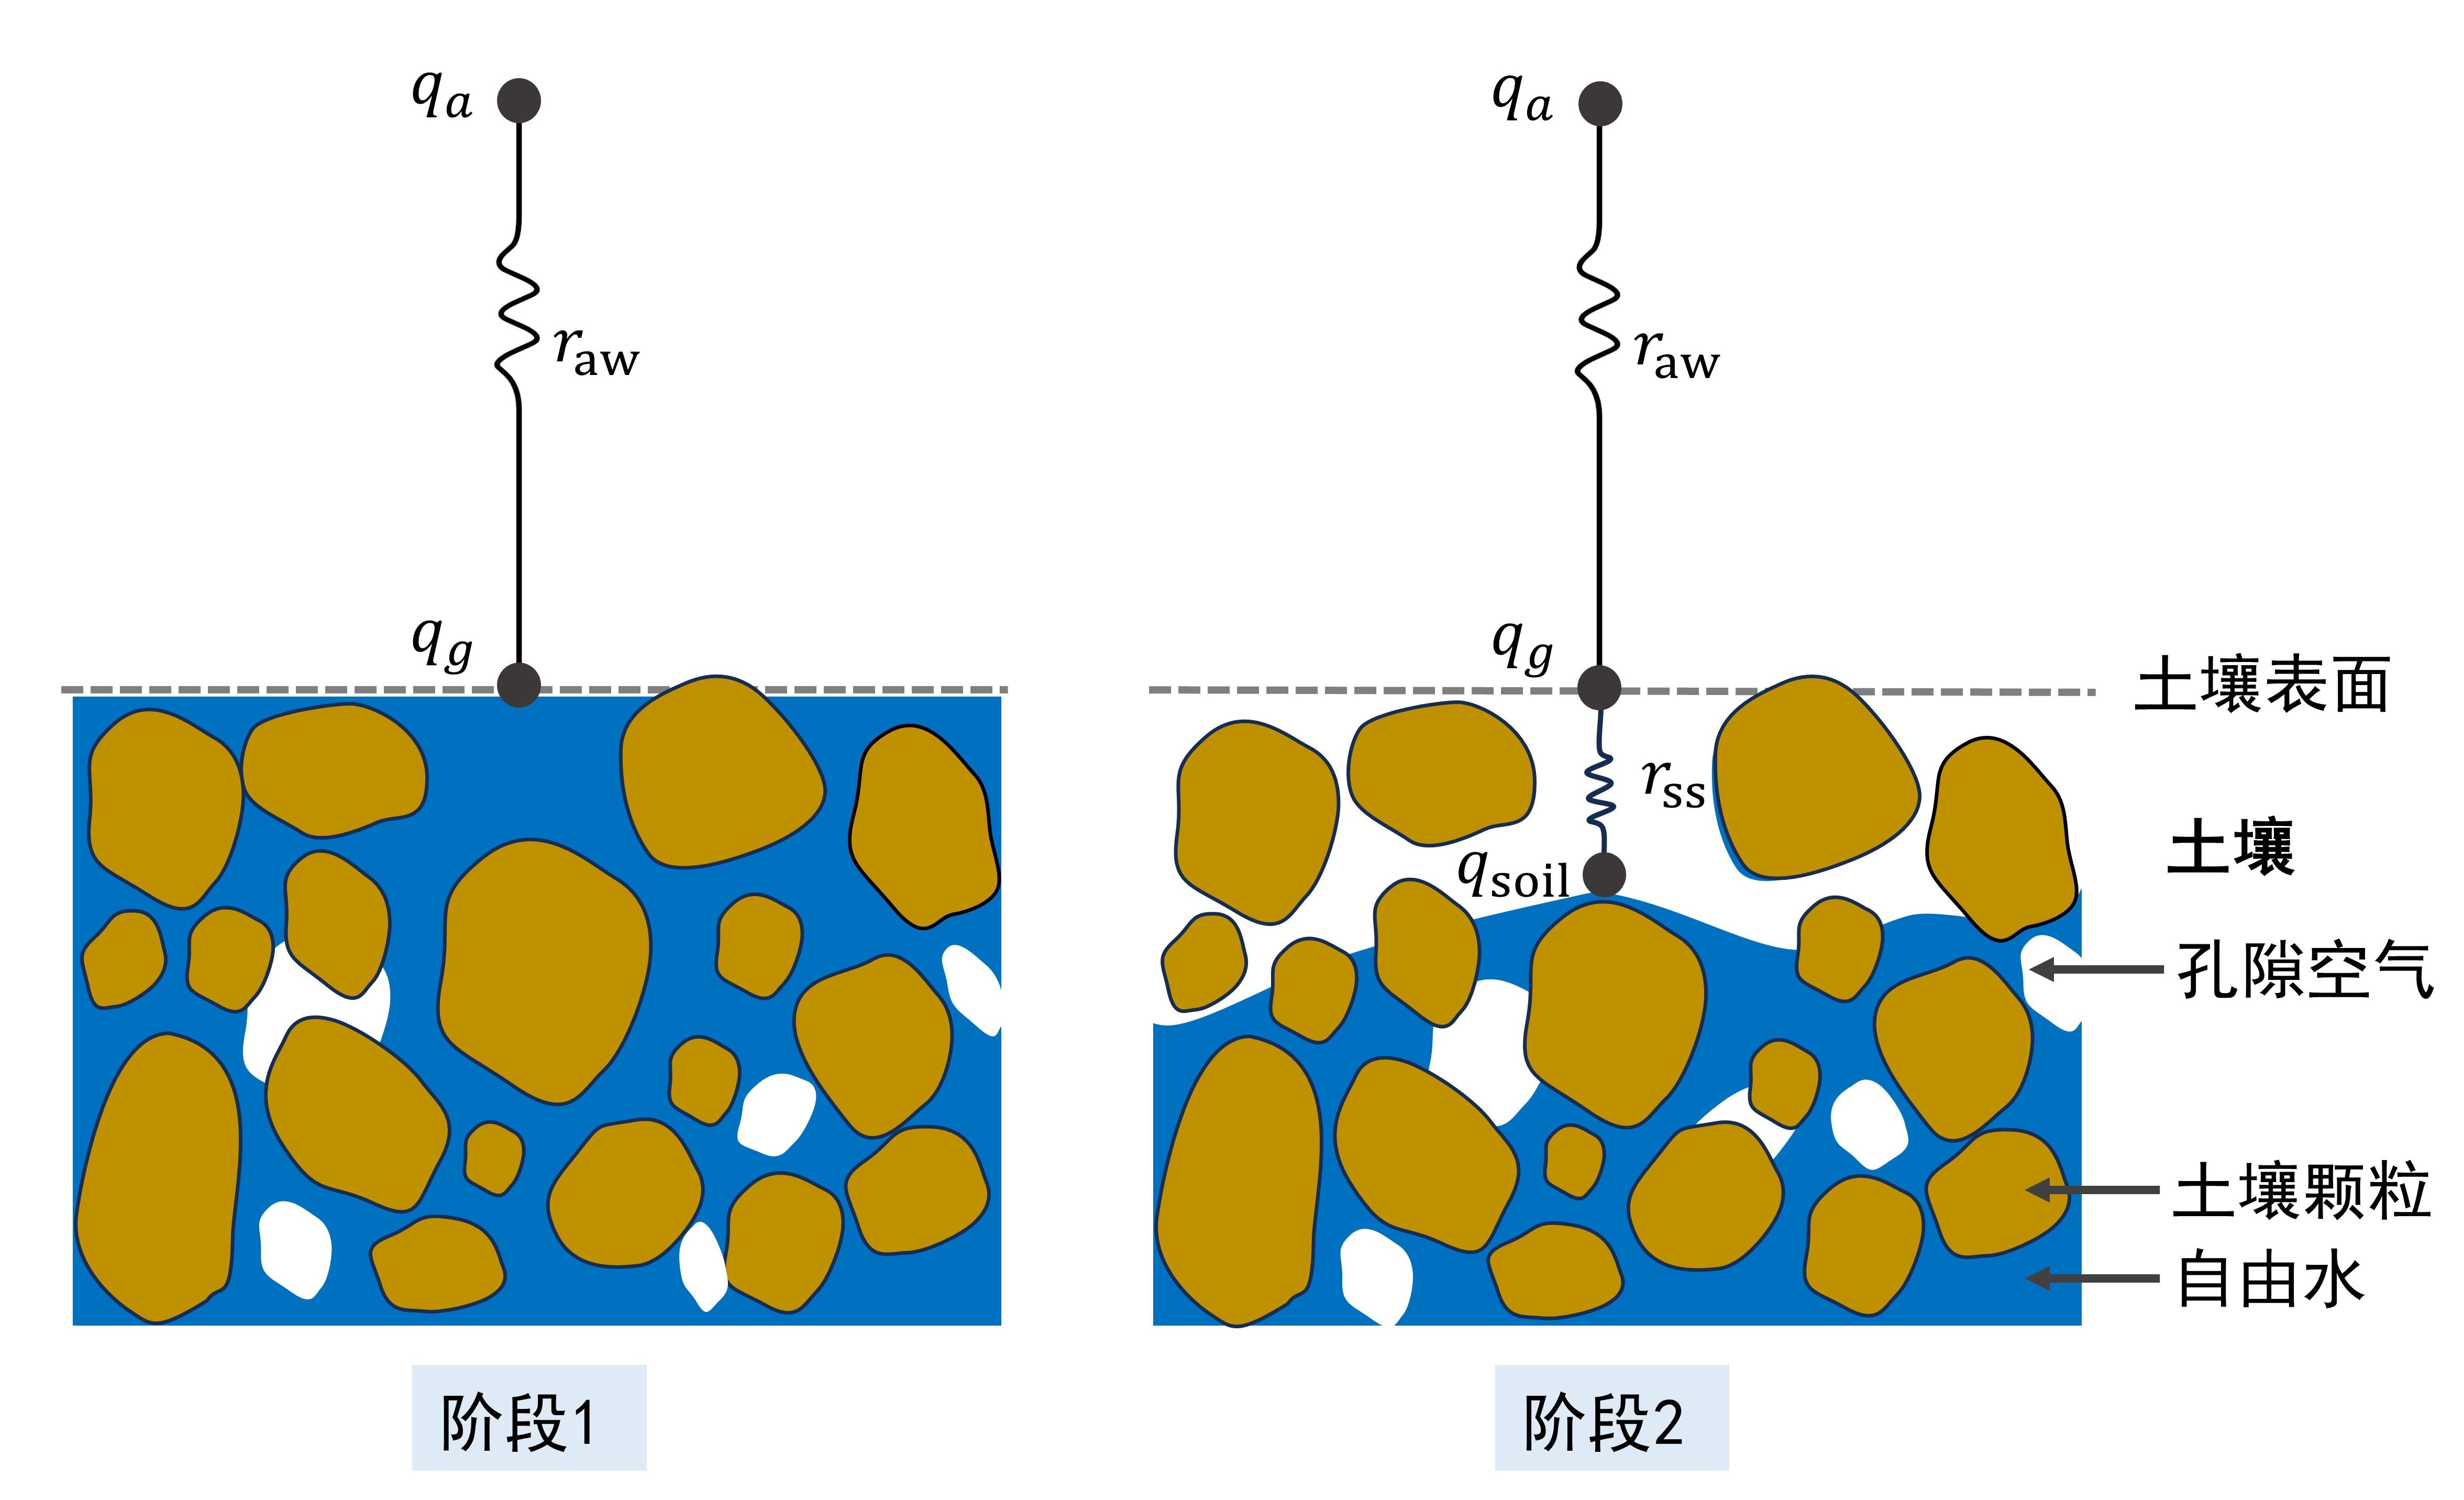
\includegraphics[width=0.95\textwidth]{Figures/地表湍流交换过程/土壤阻抗示意图_v4.png}
    \caption[土壤阻抗示意图]{土壤阻抗示意图。其中,\(q_{\mathrm{a}}\)、\(q_{\mathrm{g}}\)、\(q_{\mathrm{soil}}\)分别代表一定高度空气比湿(高度取决于有无植被及采用的阻抗交换网络)、地表比湿和土壤孔隙中水附近的比湿,\(r_{\mathrm{aw}}\)、\(r_{\mathrm{ss}}\)分别代表空气动力学阻抗和土壤阻抗}
    \label{fig:土壤阻抗示意图}
  \end{figure}
}

目前CoLM支持5种土壤阻抗方案,每种方案的计算表达式和模型中对应方案的选择如表~\ref{tab:土壤阻抗方案列表} 所示。如果用户需要打开土壤阻抗选项,需设置\texttt{DEF\_RSS\_SCHEME}
= {[}土壤阻抗选项{]},不打开则设置\texttt{DEF\_RSS\_SCHEME} =
0。在CoLM模型默认打开方案1。

图~\ref{fig:土壤阻抗方案差异图} 代表不同土壤含水量下阻抗方案的\(r_{\mathrm{ss}}\)和$\beta$的差异,$\beta$代表了不同方案对潜在蒸发的限制,$\beta$值越大,限制越小。当无植被覆盖时,$\beta$通过\(r_{\mathrm{ss}}\)和\(r_{\mathrm{aw}}\)计算得到:
\begin{equation}
  \beta = \frac{1}{1 + \frac{r_{\mathrm{ss}}}{r_{\mathrm{aw}}}}\
\end{equation}

在土壤特别干燥(如小于萎蔫点)和特别湿润(大于田间持水量)时,不同方案\(r_{\mathrm{ss}}\)的数值有差异,但是土壤阻抗方案的差异较小;当土壤水含量在中间状态时,土壤阻抗的方案差异较大。对不同方案的计算得到的$\beta$进行排序发现:LP92\textgreater TR13\textgreater SZ09\textgreater S92\textgreater SL14,因此SL14方案对土壤蒸发的限制最强,LP92方案限制较弱。

{
  \begin{figure}[htbp]
    \centering
    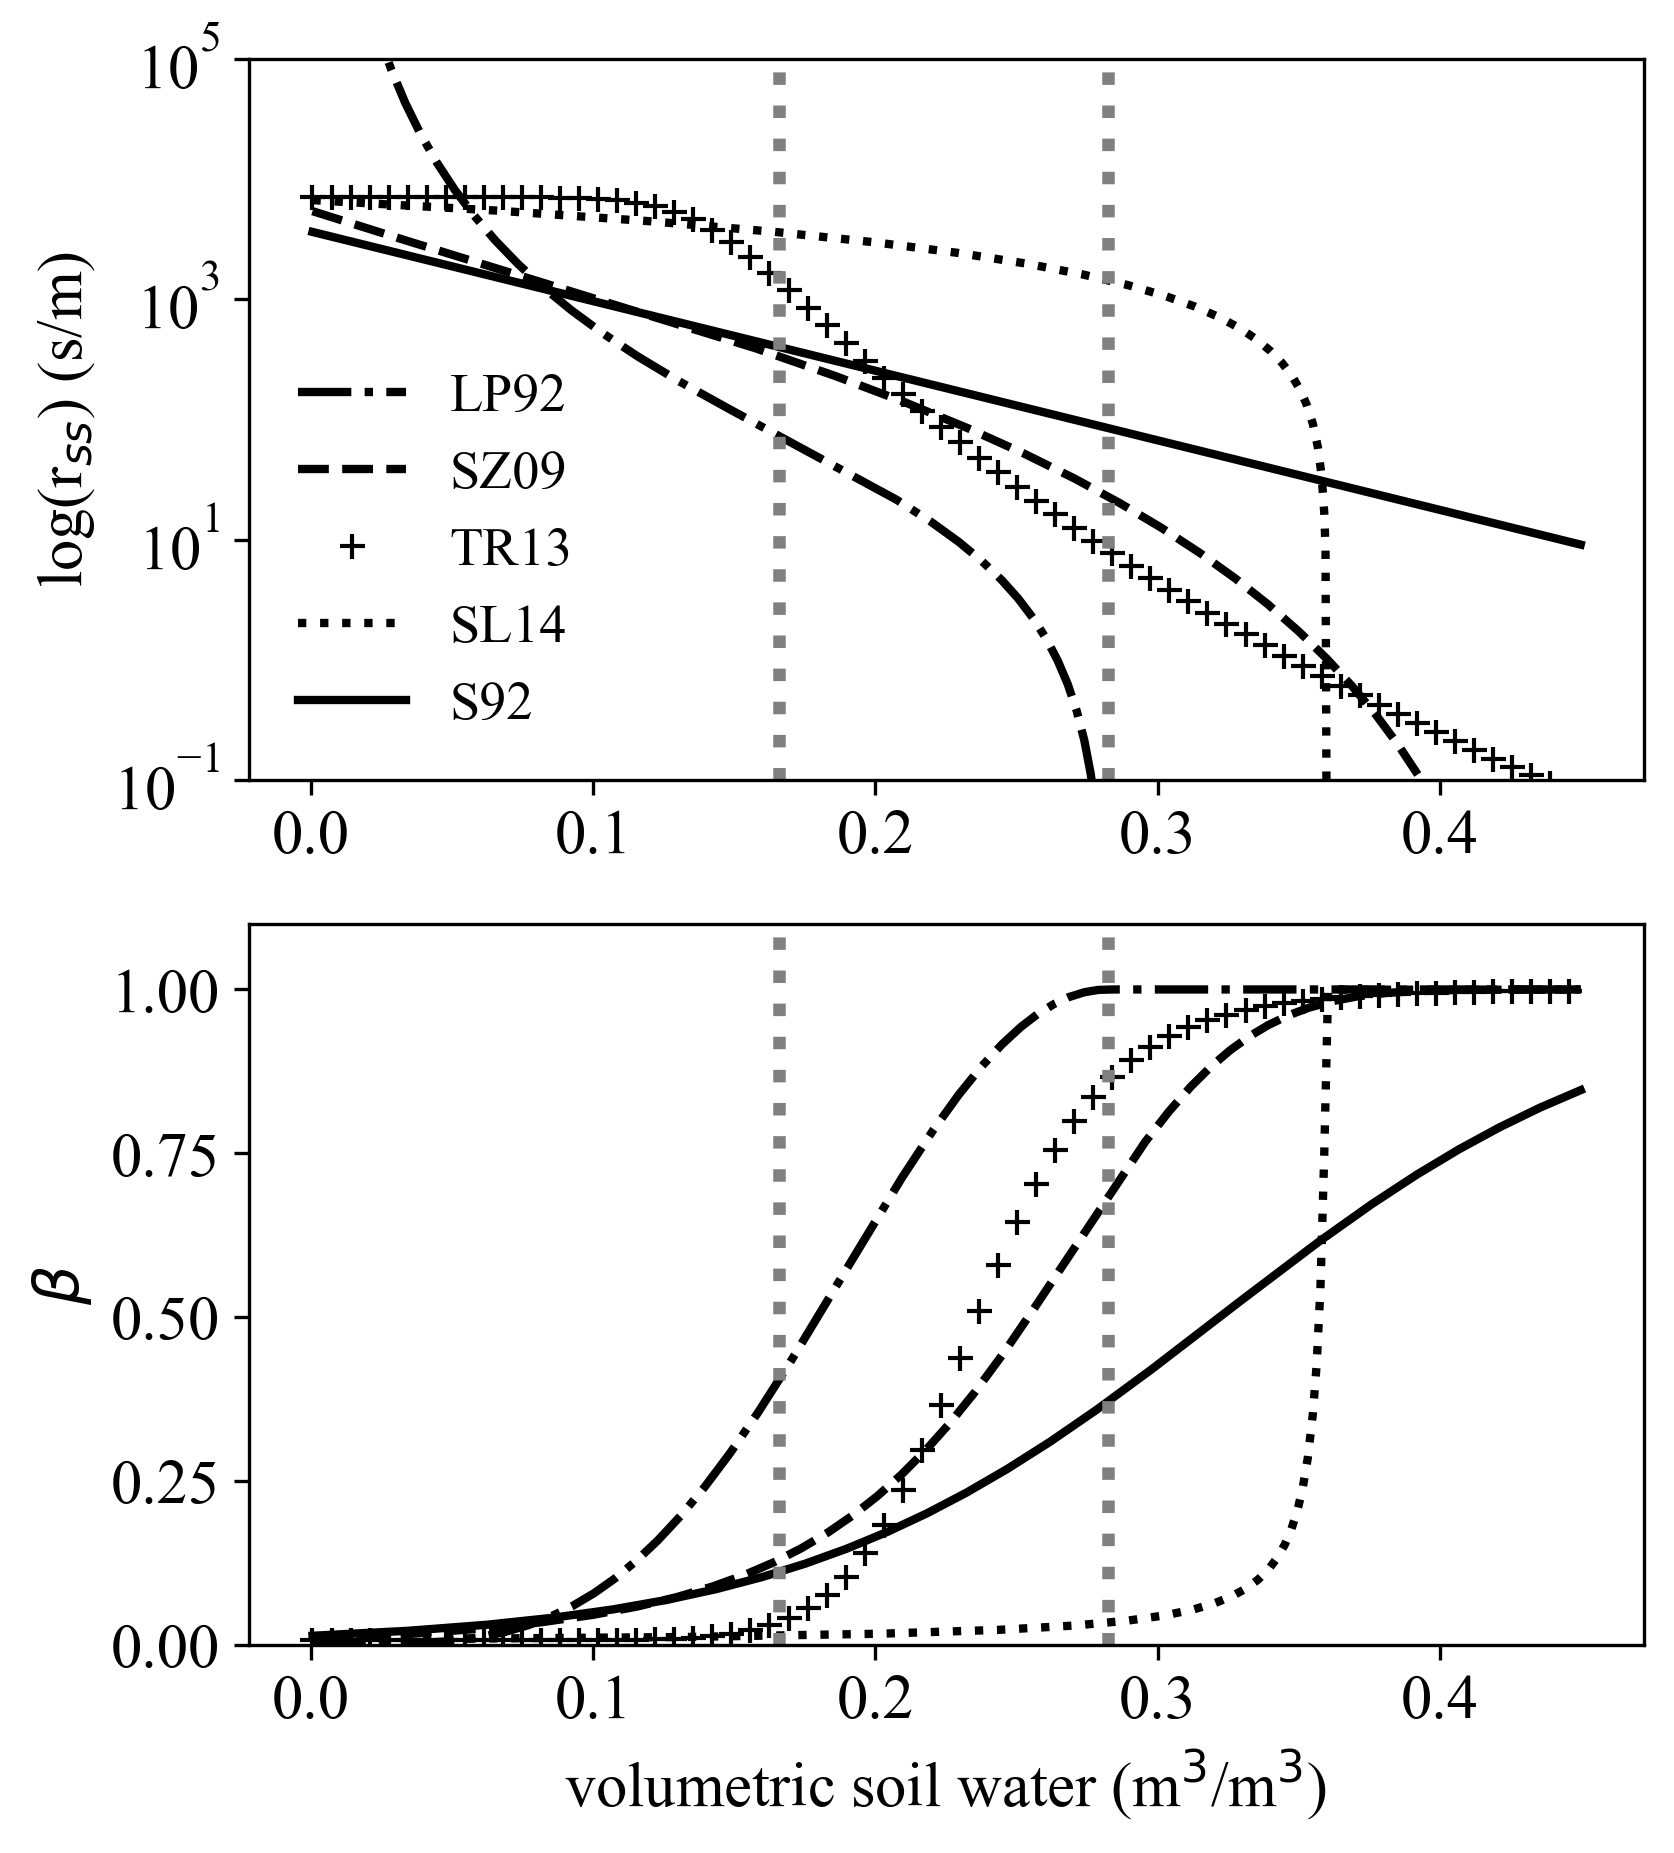
\includegraphics[width=0.7\textwidth]{Figures/地表湍流交换过程/土壤阻抗方案差异图.png}
    \caption[土壤阻抗方案差异图]{土壤阻抗方案差异图。采用Campbell的土壤参数,其中\(\theta_{\mathrm{s}}\)为0.45 \unit{m^{3}.m^{-3}},B为7.12,\(\varphi_{\mathrm{s}}\)为\num{-123} \unit {mm},土壤表层温度为282.15 K,\(K_{\mathrm{s}}\)为 \num{1.25e-6} \unit{m.s^{-1}}。设定厚度为1.75 cm,SL14方案中\(K_{\mathrm{sl}}\)为0.8,SZ09方案中\(w_{\mathrm{sz}}\)为5,\(r_{\mathrm{aw}}\)=50 \unit {s.m^{-1}}。图中灰色虚线从左到右依次为土壤萎蔫点和田间持水量时的土壤水含量}
    \label{fig:土壤阻抗方案差异图}
  \end{figure}
}

{
  \begin{landscape}
    \begin{table}[htbp]
      \caption{土壤阻抗计算方案列表}
      \label{tab:土壤阻抗方案列表}
      \begin{tabular}{@{}clll@{}}
        \toprule
        模式选项                                                                                & 土壤阻抗表达式                                                                                                                                      & 方法/假设                              & 参考文献                                   \\
        \midrule
        1                                                                                       & \(r_{\mathrm{ss}} = \frac{DSL}{D_{\mathrm{g}}}\)                                                                                                    & 菲克定律                               & \citet{sl2014}, SL14                       \\
        2                                                                                       & \(r_{\mathrm{ss}} = \frac{DSL}{D_{\mathrm{g}}}\)                                                                                                    & 菲克定律                               & \citet{sz2009}, SZ09                       \\
        3                                                                                       & \(\frac{1}{r_{\mathrm{ss}}} = \frac{1}{r_{\mathrm{g\ }}} + \frac{1}{r_{\mathrm{w\ }}}\)                                                             & 菲克定律, 达西定律                     & \citet{tang2013}, TR13                     \\
        4                                                                                       & \(\beta_{\mathrm{soil}} = \left\{ \begin{array}{r} \frac{1}{4}{\lbrack 1 - \cos(\frac{\theta_{\mathrm{1}}}{\theta_{\mathrm{fc,1}}}\pi)\rbrack}^{2} \\ 1 \end{array} \right.\ \begin{matrix}  & \theta_{\mathrm{1}} < \theta_{\mathrm{fc}} \\  & \theta_{\mathrm{1}} \geqslant \theta_{\mathrm{fc}}\text{ or }q_{\mathrm{\text{a }}} > q_{\mathrm{soil}} \end{matrix}\) & 经验拟合 & \citet{lp1992}\textsuperscript{a}, LP92 \\
        5                                                                                       & \(r_{\mathrm{ss}} = \exp\left( 8.206 - 6.0\frac{\theta_{\mathrm{1}}}{\theta_{\mathrm{s,1}}} \right)\)
                                                                                                & 经验拟合                                                                                                                                            & \citet{s1992}\textsuperscript{b}, S92 \\ \bottomrule
      \end{tabular}
      \footnotesize                                                                            \\
      \textsuperscript{a} $\beta_{\mathrm{soil}}$为限制土壤蒸发的因子,范围为{[}0-1{]},无单位 \\
      \textsuperscript{b} Sellers原方案为$r_{\mathrm{ss}} = \exp\left( 8.206 - 4.255\frac{\theta_{\mathrm{1}}}{\theta_{\mathrm{s,1}}} \right)\ $,然而~\citet{sz2009}指出该方案在土壤水饱和时,$r_{\mathrm{ss}}$计算值不合理,为了降低土壤较为湿润的$r_{\mathrm{ss}}$,Noah-MP v5对其进行修正为$r_{\mathrm{ss}} = \exp\left( 8.206 - 6.0 \frac{{\theta}_{\mathrm{1}}}{\theta_{\mathrm{s,1}}} \right)$
    \end{table}
  \end{landscape}
}

以下针对不同的方案进行简单介绍。

\begin{enumerate}
    \def\labelenumi{\arabic{enumi}.}
  \item
    SL14方案
%\end{enumerate}

    在SL14方案中,\(r_{\mathrm{ss}}\)是通过参数化土壤干燥层厚度\(DSL\)和水汽分子在土壤中的扩散系数\(D_{\mathrm{g}}\)得到的。其中,\(DSL\)的计算由下式给出
    \begin{equation}
      DSL = \begin{cases}
        \Delta z_{1} \times \frac{\theta_{\mathrm{init,1\ \ }} - \theta_{1}}{\theta_{\mathrm{init,2\ \ }} - \theta_{\mathrm{a}}} & \theta_{1} < K_{\mathrm{sl}}\theta_{\mathrm{s,1}} \\
        0   & \theta_{1} \geqslant K_{\mathrm{sl}}\theta_{\mathrm{s,1}}
      \end{cases}
    \end{equation}
    其中,$\Delta z_{1}$ 代表第一层的土壤厚度 (\unit{m}),\(\theta_{\mathrm{init,1}}\)和\(\theta_{\mathrm{init,2}}\)代表干燥层启动时的土壤体积含水量 (\unit{m^{3}.m^{-3}}),计算为:
    \begin{equation}
      \theta_{\mathrm{init,1}} = K_{\mathrm{sl}}\left(\theta_{\mathrm{s,1}} - \theta_{\mathrm{ice,1}} \right)
    \end{equation}
    \begin{equation}
      \theta_{\mathrm{init,2}} = K_{\mathrm{sl}}\theta_{\mathrm{s,1}}\
    \end{equation}
    \(\theta_{1}\)代表第一层土壤体积含水量\((\unit{m^{3}.m^{-3}})\),\(\theta_{\mathrm{s,1}}\)为第一层土壤的饱和体积含水量\((\unit{m^{3}.m^{-3}})\),\(\theta_{\mathrm{ice,1}}\)为第一层土壤冰的体积含水量\((\unit{m^{3}.m^{-3}})\),\(\theta_{\mathrm{a}}\)代表风干后即\(\psi_{\mathrm{a}} = - 10^{7}\) mm时的土壤体积含水量\((\unit{m^{3}.m^{-3}})\),\(K_{\mathrm{sl}}\)为人为设定的参数,在CoLM中,按照~\citet{sl2014}文章中的测试,$K_{\mathrm{sl}}=0.8$。

    水汽分子在土壤中的扩散系数\(D_{\mathrm{g}}\)则是通过计算水汽分子在空气中的扩散系数\(\ D_{0}\)和水汽穿过土壤基质的路径\(\tau\)得到的,计算如下:
    \begin{equation}
      D_{\mathrm{g}} = D_{0} \times \tau\
    \end{equation}
    \(D_{0\ }\)代表水汽分子在空气中的扩散系数\((\unit{m^{2}.s^{- 1}})\),计算如下:
    \begin{equation}
      D_{0\ } = 2.12 \times 10^{- 5}\left( \frac{T_{1}}{273.15} \right)^{1.75}\
    \end{equation}
    其中,\(T_{1}\)代表土壤表层的温度(K)。

%\begin{enumerate}
%\def\labelenumi{\arabic{enumi}.}
%\setcounter{enumi}{1}
  \item
    SZ09方案
%\end{enumerate}

    SZ09方案与SL14方案同样都是基于土壤干燥层中水汽扩散的菲克定律得到。只是两者对于\(DSL\)的计算方式不同,SZ09方案中\(DSL\)的计算如下所示:
    \begin{equation}
      DSL = \Delta z_{1} \times \frac{{\mathrm e}^{\left( 1 - \frac{\theta_{1}}{\theta_{\mathrm{s,1}}} \right)^{w_{\mathrm{sz}}}} - 1}{e - 1}\
    \end{equation}
    其中,\(w_{\mathrm{sz}}\)为人为设定的参数,在CoLM中,按照~\citet{sz2009}中的测试,\(w_{\mathrm{sz}}\)设置为5。\(D_{\mathrm{g}}\)、\(\tau\)和\(D_{0\ }\)的计算与SL14方案相同。

%\begin{enumerate}
%\def\labelenumi{\arabic{enumi}.}
%\setcounter{enumi}{2}
  \item
    TR13方案
%\end{enumerate}

    与SL14方案和SZ09方案仅仅只考虑土壤干燥层中的水汽扩散不同,TR13方案同时考虑了土壤层中液态水和气态水的扩散。TR13方案计算的\(r_{\mathrm{ss}}\)进一步被划分为\(r_{\mathrm{g\ }}\)代表土壤孔隙中水汽扩散的阻抗 (\unit{s.m^{-1}})和\(r_{\mathrm{w\ }}\)代表液态水挥发阻抗(\unit{s.m^{-1}})。它们的计算如下:
    \begin{equation}
      \frac{1}{r_{\mathrm{\mathrm{g}}}} = \frac{2D_{\mathrm{g\ }}\varepsilon_{1}}
      {\Delta z_{1}}\ \
    \end{equation}
    \begin{equation}
      \frac{1}{r_{\mathrm{w}}} = \frac{2D_{\mathrm{w}}Bunsen\theta_{1}}
      {\Delta z_{1}}\
    \end{equation}
    其中,\(D_{\mathrm{w\ }}\)代表液态水的扩散系数(\unit{m^{2}.s^{- 1}}),\(\varepsilon_{1}\)代表第一层土壤中空气填充的孔隙空间(\unit{m^{3}.m^{-3}}),\(Bunsen\)为Bunsen溶解系数,计算如下:
    \begin{equation}
      D_{\mathrm{w}} = K_{1}\frac{\partial\varphi_{1}}{\partial\theta_{1}}\
    \end{equation}
    在Campbell土壤水力模型中,\(\frac{\partial\varphi_{1}}{\partial\theta_{1}}\)计算为:
    \begin{equation}
      \frac{\partial\varphi_{1}}{\partial\theta_{1}}\  = - \frac{B_{1}\varphi_{1}}{\theta_{1}}\
    \end{equation}
    在van Genuchten土壤水力模型中,\(\frac{\partial\varphi_{1}}{\partial\theta_{1}}\)计算为:
    \begin{equation}
      S_{1} = {\lbrack 1 + ( - \alpha\varphi_{1})^{n}\rbrack}^{- m}(\alpha > 0)
    \end{equation}
    \begin{equation}
      m = 1-\frac{1}{n}
    \end{equation}
    \begin{equation}
      \frac{\partial\varphi_{1}}{\partial\theta_{1}} = - \frac{m - 1}{\alpha m\left( \theta_{\mathrm{s,1}} - \theta_{\mathrm{r,1}} \right)}S_{1}^{- \frac{1}{m}}\left( 1 - S_{1}^{\frac{1}{m}} \right)^{- m}\
    \end{equation}
    \begin{equation}
      \varepsilon_{1} = \theta_{\mathrm{s,1}} - \ \theta_{\mathrm{a}}\
    \end{equation}
    \begin{equation}
      Bunsen = \ \frac{\rho_{\mathrm{liq}}}{\rho_{\mathrm{vap}}} = \frac{\rho_{\mathrm{liq}}}{\rho_{\mathrm{a}} \times q_{\mathrm{soil}}}\
    \end{equation}
    其中,\(\rho_{\mathrm{liq}}\)为液态水密度(\unit{{kg}.m^{-3}}),\(\rho_{\mathrm{a}}\)为空气密度(\unit{{kg}.m^{-3}}),$\alpha$、$m$ 和 $n$为曲线参数。

%\begin{enumerate}
%\def\labelenumi{\arabic{enumi}.}
%\setcounter{enumi}{3}
  \item
    LP92方案
%\end{enumerate}

    与前三个方案不同,LP92方案直接计算\(\beta_{\mathrm{soil}}\),\(\beta_{\mathrm{soil}}\)是将潜在蒸发降到实际蒸发的经验因子,范围为{[}0,1{]},如表~\ref{tab:土壤阻抗方案列表} 所示。\(\theta_{\mathrm{fc,1}}\)为第一层土壤的田间持水量(\unit{m{^3}.m^{-3}}),即土壤水势为\qty{-3399}{mm}时的土壤含水量。

%\begin{enumerate}
%\def\labelenumi{\arabic{enumi}.}
%\setcounter{enumi}{4}
  \item
    S92方案
%\end{enumerate}

    利用土壤水含量经验指数关系计算\(r_{\mathrm{ss}}\),如表~\ref{tab:土壤阻抗方案列表} 所示。
%
\end{enumerate}

对于方案1--3中\(\tau\)的表达式,CoLM提供了6种方案,具体见表~\ref{tab:tau方案列表}。其中,\(\varepsilon_{1}\)代表第一层土壤中空气填充的孔隙空间(\unit{m{^3}.m^{-3}}),\(\varepsilon_{100}\)代表在土壤水势为\num{-1000} mm时的空气填充的孔隙空间(\unit{m{^3}.m^{-3}})。
图~\ref{fig:tau方案差异图} 表明了不同\(\tau\)方案的差异,不同\(\tau\)方案的\(r_{\mathrm{ss}}\)数值有一定差异,但是$\beta$差异不大。

{
  \begin{table}[htbp]
    \centering
    \caption{CoLM可选用$\tau$方案列表}
    \label{tab:tau方案列表}
    \begin{tabular}{lcc}
      \toprule
      模式选项 & 表达式 & 参考文献 \\
      \midrule
      1 &
      \(\varepsilon_{1}^{2} \times {(\frac{\varepsilon_{1}}{\theta_{\mathrm{s,1}}})}^{3/B_{1}}\)
      & \citet{BBC1999} BBC \\
      2 & \(0.66 \times \varepsilon_{1}{\times (\frac{\varepsilon_{1}}{\theta_{\mathrm{s,1}}})}\)
      & \citet{moldrup2000} P\_WLR \\
      3 & \(\varepsilon_{1}^{3/2} \times (\frac{\varepsilon_{1}}{\theta_{\mathrm{s,1}}})\)
      & \citet{moldrup2000} MA\_WLR \\
      4 & \(\varepsilon_{1}^{4/3} \times (\frac{\varepsilon_{1}}{\theta_{\mathrm{s,1}}})\)
      & \citet{moldrup2000} MI\_WLR \\
      5 & \(\varepsilon_{1}^{4/3} \times {(\frac{\varepsilon_{1}}{\theta_{\mathrm{s,1}}})}^{2}\)
      & \citet{millington_permeability_1961} MQ \\
      6 & \({\theta_{\mathrm{s,1}}}^{2} \times {(\frac{\varepsilon_{1}}{\theta_{\mathrm{s,1}}})}^{2 + \frac{\log\varepsilon_{100}^{\frac{1}{4}}}{\log\frac{\varepsilon_{100}}{\theta_{\mathrm{s,1}}}}}\) & \citet{POE2005} POE \\ \bottomrule
    \end{tabular}
  \end{table}
}

{
  \begin{figure}[htb]
    \centering
    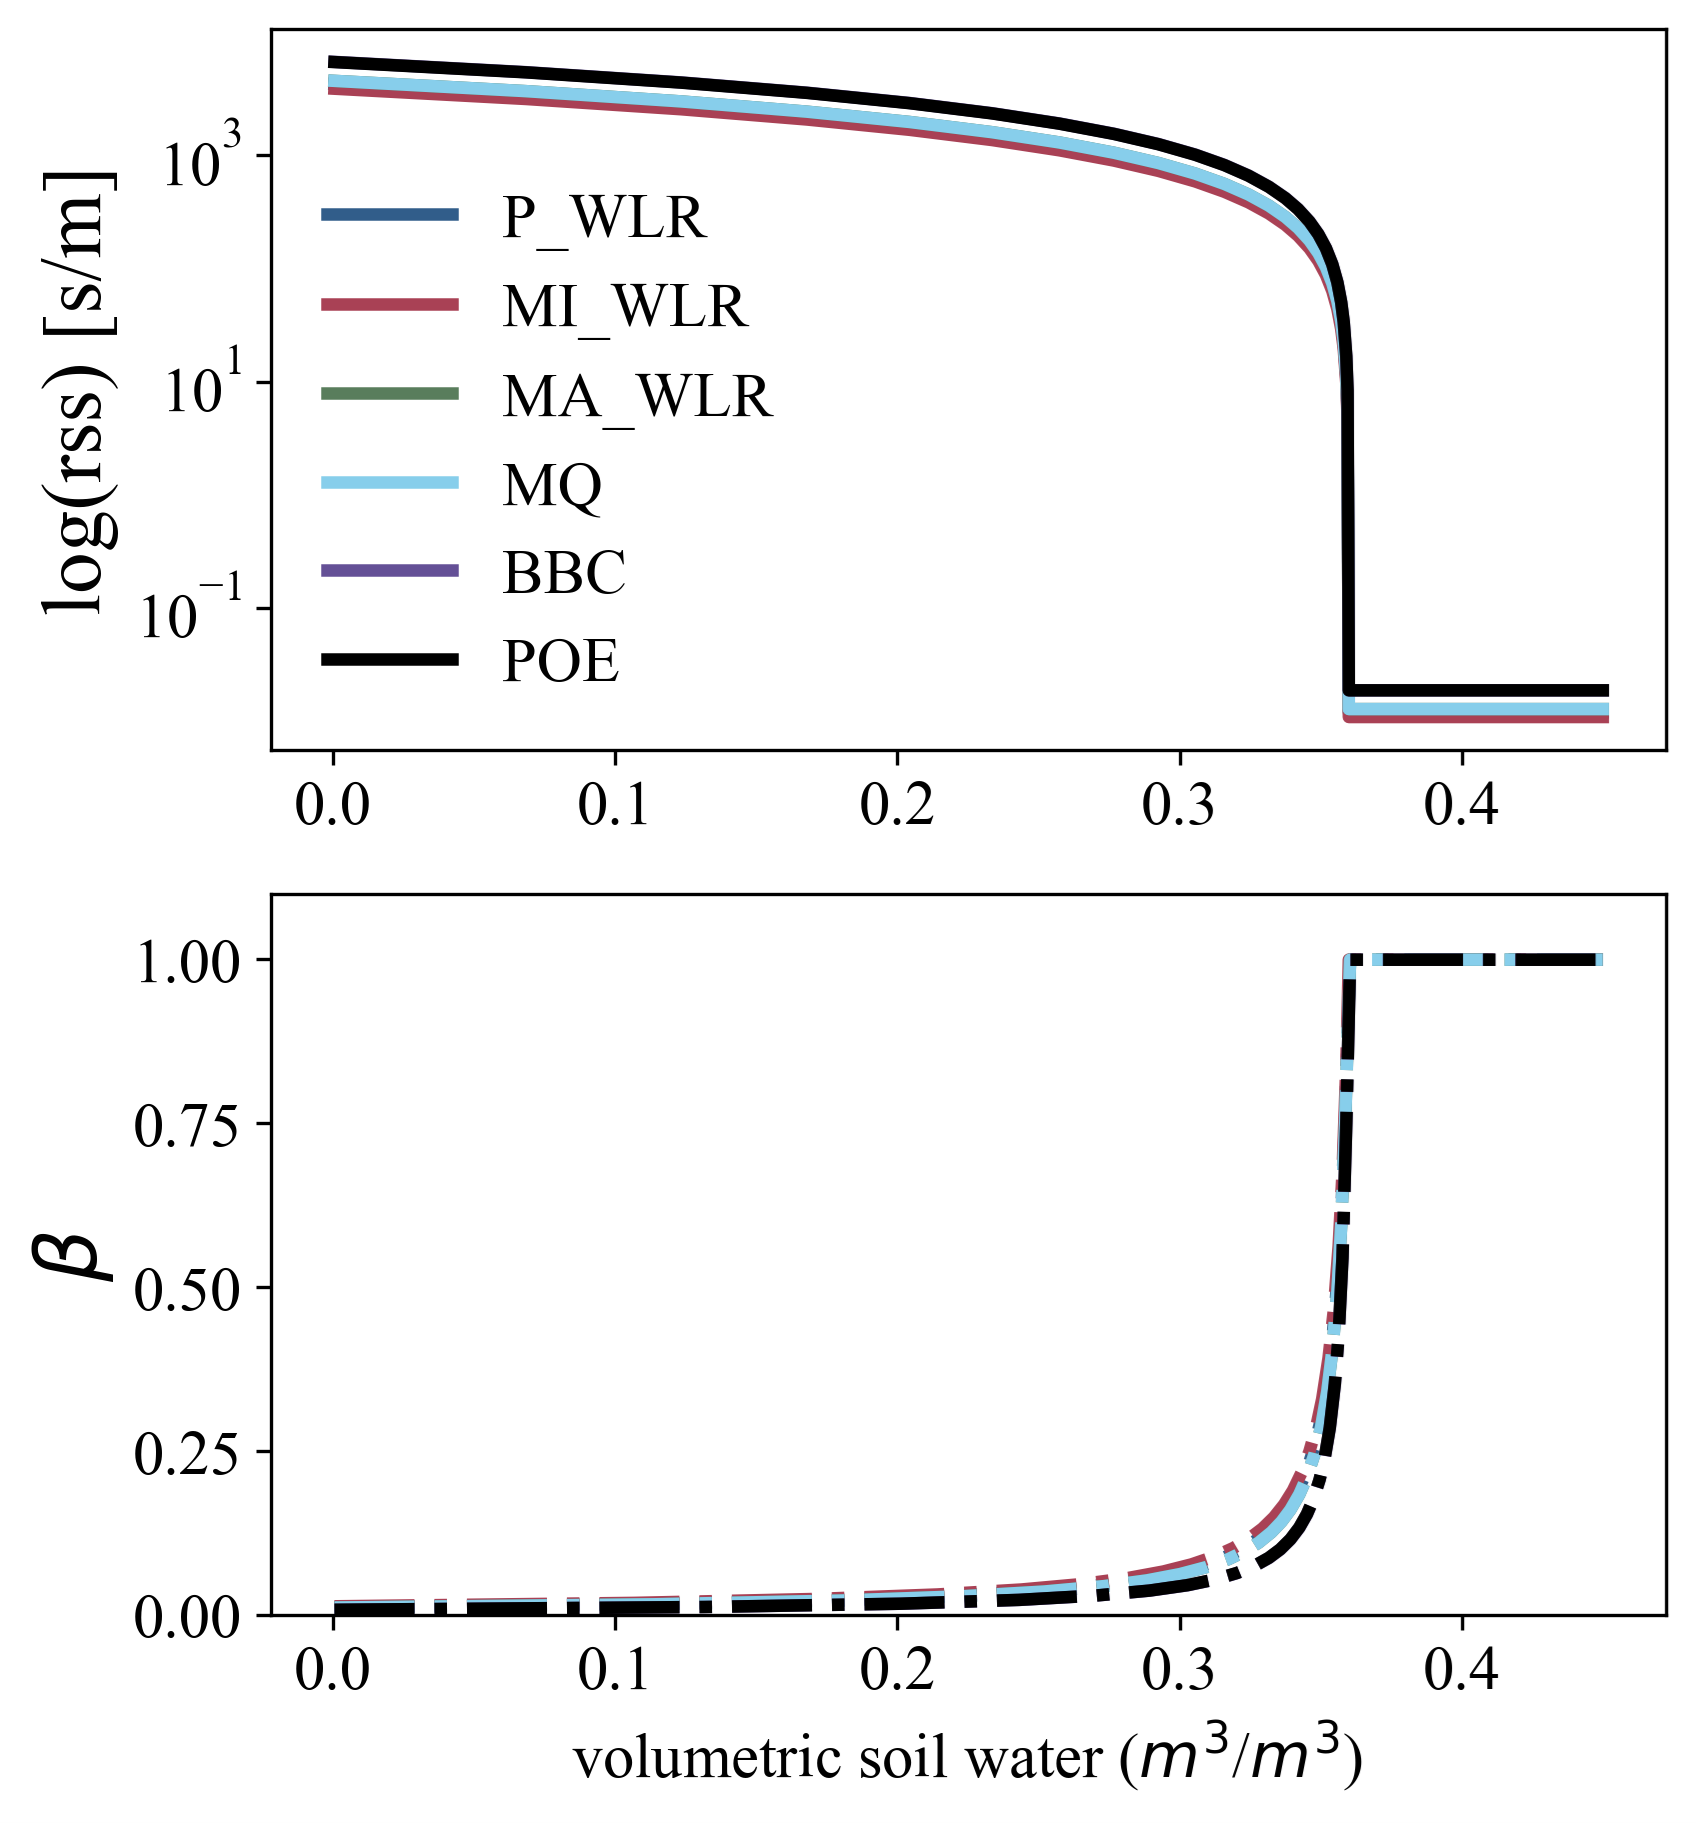
\includegraphics[width=0.7\textwidth]{Figures/地表湍流交换过程/tau方案差异图.png}
    \caption[\(\ \tau\)方案差异图]{$\tau$方案差异图。参数设置与图~\ref{fig:土壤阻抗方案差异图} 参数设置相同,土壤阻抗方案为SL14方案}
    \label{fig:tau方案差异图}
  \end{figure}
}

土壤阻抗方案1--3需要计算\(\tau\),而方案4和5无需计算\(\tau\)。当开启Campbell土壤参数方案时,所有\(\tau\)方案都可以被选取;当开启van Genuchten方案时,由于van Genuchten参数方案没有Campbell参数方案的B参数,因此\(\tau\)方案的方案1不适用van Genuchten土壤参数方案,其余方案都可以被选取。在CoLM模型中,当开启Campbell土壤参数方案时,\(\tau\)的默认选项为1;开启van Genuchten土壤参数方案时,\(\tau\)的默认选项为6。\(\tau\)的选项可直接在源代码\texttt{MOD\_SoilSurfaceResistance.F90}中进行修改。

土壤阻抗方案仅在地面非凝结或凝华时有效。当使用土壤阻抗方案为1--3、5时,在无植被覆盖下地面蒸发水汽通量\(E_{\mathrm{g}}\)即公式~\eqref{Eg} 修改为:
\begin{equation}
  E_{\mathrm{g}}=-\rho_{\mathrm{a}} \frac{q_{\mathrm{a}}-q_{\mathrm{g}}}{r_{\mathrm{a w}} + r_{\mathrm{s s}}}
\end{equation}
地面蒸发相对地面温度的变化率,即公式~\eqref{Eg/Tg_1} 修改为:
\begin{equation}
  \frac{\partial E_{\mathrm{g}}}{\partial T_{\mathrm{g}}}= \frac{\rho_{\mathrm{a}}}{r_{\mathrm{a w}} + r_{\mathrm{s s}}} \frac{{\rm d} q_{\mathrm{g}}}{{\rm d} T_{\mathrm{g}}}
\end{equation}
在有植被覆盖下,地面与植被冠层周围空气间水汽通量\(E_{\mathrm{g}}\),即公式~\eqref{eq:Eg} 修改为:
\begin{equation}
  E_{\mathrm{g}}=-\rho_{\mathrm{a}} \frac{q_{\mathrm{s}}-q_{\mathrm{g}}}{r_{\mathrm{a w}}^{\prime}+r_{\mathrm{ss}}}
\end{equation}
$c_{\mathrm {g}}^w=\frac{1}{r_{\mathrm{aw}}^\prime}$修改为$c_{\mathrm {g}}^w=\frac{1}{r_{\mathrm{aw}} ^\prime+r_{\mathrm{ss}}}$,
地面蒸发相对地表温度的变化率,即公式~\eqref{Eg/Tg_2} 修改为:
\begin{equation}
  \frac{\partial E_{\mathrm{g}}}{\partial T_{\mathrm{g}}}=
  \frac{\rho_{\mathrm{a}}}{r_{\mathrm{a w}}^{\prime} + r_{\mathrm{s s}}} \frac{c_{\mathrm{a}}^{w}+c_{\mathrm{v}}^{w}}{c_{\mathrm{a}}^{w}+c_{\mathrm{g}}^{w}+c_{\mathrm{v}}^{w}} \frac{{\rm d} q_{\mathrm{g}}}{{\rm d} T_{\mathrm{g}}}
\end{equation}

当使用土壤阻抗方案4时,在无植被覆盖下水汽通量\(E_{\mathrm{g}}\),即公式~\eqref{Eg} 修改为:
\begin{equation}\label{Eg_modify}
  E_{\mathrm{g}}=-\rho_{\mathrm{a}}\beta_{\mathrm{soil}} \frac{q_{\mathrm{a}}-q_{\mathrm{g}}}{r_{\mathrm{a w}}}
\end{equation}
地面蒸发相对地面温度的变化率即公式~\eqref{Eg/Tg_1} 修改为:
\begin{equation}
  \frac{\partial E_{\mathrm{g}}}{\partial T_{\mathrm{g}}}= \frac{\rho_{\mathrm{a}} \beta_{\mathrm{soil}}}{r_{\mathrm{a w}} } \frac{{\rm d} q_{\mathrm{g}}}{{\rm d} T_{\mathrm{g}}}
\end{equation}
在有植被覆盖下地面与植被冠层周围空气间水汽通量\(E_{\mathrm{g}}\),即公式~\eqref{eq:Eg} 修改为:
\begin{equation}
  E_{\mathrm{g}}=-\rho_{\mathrm{a}} \beta_{\mathrm{soil}} \frac{q_{\mathrm{s}}-q_{\mathrm{g}}}{r_{\mathrm{a w}}^{\prime}}
\end{equation}
$c_{\mathrm {g}}^w=\frac{1}{r_{\mathrm{aw}}^\prime}$修改为$c_{\mathrm {g}}^w=\frac{\beta_{\mathrm{soil}}}{r_{\mathrm{aw}}^\prime}$,
地面蒸发相对地面温度的变化率,即公式~\eqref{Eg/Tg_2} 修改为:
\begin{equation}
  \frac{\partial E_{\mathrm{g}}}{\partial T_{\mathrm{g}}}=
  \frac{\rho_{\mathrm{a}} \beta_{\mathrm{soil}}}{r_{\mathrm{a w}}^{\prime}} \frac{c_{\mathrm{a}}^{w}+c_{\mathrm{v}}^{w}}{c_{\mathrm{a}}^{w}+c_{\mathrm{g}}^{w}+c_{\mathrm{v}}^{w}} \frac{{\rm d} q_{\mathrm{g}}}{{\rm d} T_{\mathrm{g}}}
\end{equation}
